\documentclass[12pt,a4paper]{article}

\usepackage[utf8]{inputenc}
\usepackage{mathtools}
\usepackage{amssymb}
\usepackage[framemethod=TikZ]{mdframed}
\usepackage{amsmath}
\usepackage[most]{tcolorbox}
\usepackage{fancyhdr}
\usepackage{geometry}
\usepackage{setspace}
\usepackage{framed}
\usepackage{xcolor}
\usepackage{hyperref}

\geometry{a4paper, left=2cm, right=2cm, bottom=2cm, top=2cm}

\pagestyle{fancy}
\fancyhead{}
\fancyhead[L]{\textsl{\leftmark}}
\fancyhead[R]{\textsl{\rightmark}}
\fancyfoot{}
\fancyfoot[C]{\thepage}
%\renewcommand{\headrulewidth}{0pt}
\renewcommand{\footrulewidth}{0pt}

\definecolor{darkblue}{HTML}{003472}
\definecolor{lightblue}{HTML}{70f3ff}
\definecolor{red}{HTML}{da291c}
\definecolor{lightred}{HTML}{f47983}
\definecolor{green}{HTML}{057748}
\definecolor{lightgreen}{HTML}{a4e2c6}
\definecolor{gray}{HTML}{758a99}
\definecolor{lightgray}{HTML}{41555d}
\definecolor{lightblack}{HTML}{424c50}
\definecolor{orange}{HTML}{9b4400}
\definecolor{yellow}{HTML}{ffa631}
\definecolor{white}{HTML}{f0fcff}
\definecolor{purple}{HTML}{6558B1}

\hypersetup{
	colorlinks = false,
	bookmarks = true,
	bookmarksnumbered = true,
	pdfborder = 001,
	linkcolor = purple
}


\tcbuselibrary{skins, breakable, theorems}
\newtcolorbox{df}[2][]{
	colback=lightgray!5, colframe=lightblack,colbacktitle=lightblack, coltitle=white,title={#2},fonttitle=\bfseries,breakable
}

\newtcolorbox{thm}[2][]{
	colback=lightblue!5, colframe=darkblue,colbacktitle=darkblue, coltitle=white,title={#2},fonttitle=\bfseries,breakable
}

\newtcolorbox{eg}[2][]{
	colback=lightgreen!5, colframe=green,colbacktitle=green, coltitle=white,title={#2},fonttitle=\bfseries,breakable
}

\newtcolorbox{prf}[2][]{
	colback=orange!5, colframe=orange,colbacktitle=orange, coltitle=white,title={#2},fonttitle=\bfseries,breakable
}

\newtcolorbox{ext}[2][]{
	colback=yellow!5, colframe=yellow,colbacktitle=yellow, coltitle=white,title={#2},fonttitle=\bfseries,breakable
}

\newtcolorbox{rmk}[2][]{
	colback=lightred!5, colframe=red,colbacktitle=red, coltitle=white,title={#2},fonttitle=\bfseries,breakable
}
\tcbset{highlight math/.append style={left=0mm,right=0mm,top=0mm,bottom=0mm, colframe=white}}


\title{Emory University\\\textbf{MATH 112Z - Calculus II Learning Notes}}
\author{Jiuru Lyu}
\date{\today}

\linespread{1.25}

\def\Z{{\mathbb{Z}}}
\def\R{{\mathbb{R}}}
\def\C{{\mathbb{C}}}
\def\Q{{\mathbb{Q}}}
\def\E{{\mathbb{E}}}
\def\d{{\mathrm{d}}}
\def\i{{\mathrm{i}}}
\def\RE{{\mathrm{Re}}}
\def\IM{{\mathrm{Im}}}
\def\Arg{{\mathrm{Arg}}}
\def\cis{\mathrm{cis}}
\def\qed{\rightline{$\blacksquare$}}
\def\ddx{\frac{\d}{\d x}}
\def\dydx{\frac{\d y}{\d x}}
\def\dx{\d x}
\def\DNE{\mathrm{D.N.E.}}

\begin{document}
\maketitle
\tableofcontents
\newpage

\section{Preface}
These is my personal notes for Emory University MATH 112Z Calculus II course. 

After mastering Calculus I (which covers contents concerning limits, differentiation, and basic integration), this course focuses on integration technics, differential equations, series, and polar coordinates. The book used for this course is \textit{Single Variable Calculus Early Transcendentals, 8th Edition} by James Stewart. 

Throughout this personal note, I use special ``tcolorboxes" to differentiate different contents, including definitions, theorems, proofs, examples, extensions, and remarks. To be more specific: 
\begin{df}{Terminology}
	This is a \textbf{definition}.	
\end{df}
\begin{thm}{Theorem Name}
	This is a \textbf{theorem}.	
\end{thm}
\begin{eg}{Example Number}
	This is the \textit{question} part of an \textbf{example}. \\
	\noindent\rule[0.25\baselineskip]{\textwidth}{1pt}
	This is the \textit{answer} part of an \textbf{example}. 
\end{eg}
\begin{rmk}{Remark}
	This is a \textbf{remark} of a definition, theorem, example, or proof. 
\end{rmk}
\begin{prf}{Proof}
	This is a \textbf{proof} of a theorem. 
\end{prf}
\begin{ext}{Extension}
	This is a \textbf{extension} of a theorem, proof, or example. 	
\end{ext}

To better ace this course, it is recommended to do more questions than provided as examples under each section. Although each example is distinctive and representative, more questions and practice is still needed to deepen the understanding of this course. 

Even though I put efforts into making as few flaws as possible when encoding these learning notes, some errors may still exist in this note. If you find any, please contact me via email: \url{lvjiuru@hotmail.com}. 

I hope you will find my notes helpful when learning Calculus II, a fundamental course for other Math courses. 

\rightline{Cheers,}
\rightline{Jiuru Lyu}

\newpage
\section{Review - Pre-Calculus \& Derivative}
\subsection{Inverse Functions}
\begin{df}{Inverse Functions}
	Functions that ``undo" each other.
\end{df}
\begin{eg}{Examples of Inverse Functions}
	$$f(x)=x+1 \Longleftrightarrow f^{-1}(x)=x-1$$
	$$f(x)=2x \Longleftrightarrow f^{-1}(x)=\dfrac{1}{2}x$$
	$$f(x)=\dfrac{1}{x} \Longleftrightarrow f^{-1}(x)=\dfrac{1}{x}$$
\end{eg}
Note: Not all functions have inverses.
\begin{df}{One-to-one function}
	$f$ is an one-to-one function if: 
	$$f(x_1)\neq f(x_2)\text{ whenever }x_1\neq x_2.$$
	In df words, $f$ never have the same value twice. 
\end{df}
To testify if a function $f$ is a one-to-one function, we apply the Horizontal Line Test (HLT): 
\begin{thm}{Horizontal Line Test (HLT)}
	$f$ is one-to-one \underline{if and only if (\textit{iff})} every horizontal line intersects the graph of $f$ in \textbf{at most one} point.
\end{thm}
After knowing the Horizontal Line Test, we can have a look at the precise definition of inverse functions. 
\begin{df}{Precise Definition of Inverse Functions}
	Suppose $f$ is a function with a domain$=D_f$ and a range$=R_f$. Now consider a function $g$ with a domain$=D_g$ and a range$=R_g$. Then, $f$ and $g$ are inverses of each other \textit{iff}: 
	\begin{enumerate}
		\item $D_f=R_g$ and $D_g=R_f$;
		\item $f(g(x))=x\ \forall x\in D_g$ and $g(f(x))=x\ \forall x\in D_f$.
	\end{enumerate}
\end{df}
Here are some notes to that formal definition: 
\begin{enumerate}
	\item In order for $f$ to have an inverse, it must be one-to-one.
	\item If $f$ has an inverse $g$, then we usually write $f^{-1}(x)=g(x)$.
	\item If the point $(a,b)$ is on the graph of $f(x)$, then the point $(b,a)$ is on the graph of $f^{-1}(x)$.
	\begin{prf}{Symmetry of Inverse Functions}
		$$\begin{aligned}
			&\because (a, b)\text{ on }f(x)\\
			&\therefore f(a)=b\\
			&\text{Take the inverse on both sides, and we get: }\\
			&f^{-1}(f(a))=f^{-1}(b)\\
			&\therefore a=f^{-1}(b), \text{ i.e., }(b,a)\text{ on }f^{-1}(x)
		\end{aligned}$$ \qed
	\end{prf}
\end{enumerate}
Extending from the third point of the note, we come to the graph property of inverses. 
\begin{thm}{Graph Property of Inverses}
	If $f(x)$ has an inverse, then the graphs of $f(x)$ and $f^{-1}(x)$ are reflections of each other through the line $y=x$.
\end{thm}

\subsection{Exponentials and Logs}
Recall the graph of $y=a^x$, where $a>0$ and $a\neq 1$. When $0<a<1$, the exponential function decreases as $x$ increases. When $a>1$, the exponential function increases as $x$ increases. 
\begin{thm}{Exponentials and Logs as Inverse Functions}
	The inverse of $f(x)=a^x$ is $f^{-1}(x)=g(x)=\log_a x$, and: 
	$$D_f=(-\infty,\infty),\ D_{f^{-1}}=(0,\infty);$$
	$$R_f=(0,\infty),\ R_{f^{-1}}=(-\infty,\infty).$$
\end{thm}
\begin{ext}{Extension for the Relationship}
	$$\log_a x=y \Longleftrightarrow a^y=x: $$
	$$\begin{cases}
		a^{\log_a x}=x &\forall x\in (0,\infty)\\
		\log_a (a^x)=x &\forall x\in\R
	\end{cases}$$
	Here, what makes the domain of $x$ different is the which function $x$ firstly go through. In the first expression, $x$ firstly goes through the log function, hence having a limited domain. However, going through the exponential function first will not limit the domain of $x$.
\end{ext}
There are several properties of Logs, and the next chunk lists some of them. 
\begin{thm}{Properties of Logs}
	$$\begin{aligned}
		&\log_ax+\log_ay=\log_a(x+y) \quad
		&\log_ax^r=r\log_ax \\
		&\log_ax-\log_ay=\log_a\left(\frac{x}{y}\right) \quad
		&\log_ax=\dfrac{\log_bx}{\log_ba}
	\end{aligned}$$
\end{thm}
Natural Log is another essential concept. 
\begin{df}{Natural Log}
	Natural Logs are logarithms with base $e\approx 2.71828\cdots$\\
	We write $\log_ex=\ln x$.
\end{df}

\subsection{Derivatives}
Recall some basic rules of derivatives: 
\begin{thm}{Rules of derivatives}
	$$\begin{aligned}
		\dfrac{\d}{\d x}\left(e^x\right)&=e^x\\
		\dfrac{\d}{\d x}\left(\ln x\right)&=\dfrac{1}{x}\\
		\dfrac{\d}{\d x}\left(a^x\right)&=a^x\ln a\\
		\dfrac{\d}{\d x}\left(\log_ax\right)&=\dfrac{1}{x\ln a}
	\end{aligned}$$
\end{thm}
\begin{eg}{Find the derivative of }
	$$f(x)=\ln\left(\dfrac{\sqrt[3]{x^5-4}}{(x^2+3)(7x-10)}\right)$$
	\noindent\rule[0.25\baselineskip]{\textwidth}{1pt}
	$\boxed{\text{Method 1}}$ We can simply differentiate the function using chain and quotient rules. However, this will make the process overcomplicated. \\
	$\boxed{\text{Method 2}}$ Use properties of logarithms to simply the expression first: 
	$$\begin{aligned}
		f(x)=\ln\left[\dfrac{(x^5-4)^{1/3}}{(x^2+3)(7x-10)}\right]&=\ln\left[(x^5-4)^{\frac{1}{3}}\right]-\ln\left[(x^2+3)(7x-10)\right]\\
		&=\dfrac{1}{3}\ln(x^5-4)-\ln(x^2+3)-\ln(7x-10).
	\end{aligned}$$
	Now, we can easily compute the derivative of $f(x)$:
	$$\begin{aligned}
		f'(x)&=\dfrac{1}{3}\cdot\dfrac{1}{x^5-4}(x^5-4)'-\dfrac{1}{x^2+3}(x^2+3)'-\dfrac{1}{7x-10}(7x-10)'\\
		&=\dfrac{5x^4}{3(x^5-4)}-\dfrac{2x}{x^2+3}-\dfrac{7}{7x-10}
	\end{aligned}$$
\end{eg}

\subsection{Inverse Trigonometric Functions}
Recall the definition of inverse trigonometric functions and the restrictions on their domains. 
\begin{thm}{Domain of inverse sine function}
	The sine function $y=\sin x$ with domain$=\left[-\dfrac{\pi}{2},\dfrac{\pi}{2}\right]$ and range$=[-1,1]$ has the inverse function of $y=\sin^{-1}(x)=\arcsin(x)$ with domain$=[-1,1]$ and range$=\left[-\dfrac{\pi}{2},\dfrac{\pi}{2}\right]$.\\
	Because they are inverse of each other, we have the following properties holding true:
	$$\begin{cases}
		\sin^{-1}(\sin(x))=x\quad&\forall x\in\left[-\dfrac{\pi}{2},\dfrac{\pi}{2}\right]\\
		\sin(\sin^{-1}(x))=x\quad&\forall x\in[-1,1]
	\end{cases}$$
	Moreover, we have: 
	$$y=\sin^{-1}(x) \Longleftrightarrow \sin(y)=x,\ y\in\left[-\dfrac{\pi}{2},\dfrac{\pi}{2}\right].$$
\end{thm}
Similarly, we can define the restrictions on the domain of other inverse trigonometric functions. 

Also recall derivatives of inverse trigonometric functions. 

\newpage
\section{Integration Technics}
\subsection{Integration by Parts}
\begin{df}{Integration by Parts}
	The formula of integration by parts is given by: 
	$$\int u\ \d v=uv-\int v\ \d u$$
\end{df}
\begin{prf}{Integration by Parts}
	To begin with, we consider the product rule for differentiation: 
	$$\frac{\d}{\d x}\left(f(x)g(x)\right)=f(x)g'(x)+g(x)f'(x)$$
	The proof begins with attempting to take the integral of the both sides of this product rule.
	$$\begin{aligned}
		\d\left(f(x)g(x)\right)&=\left(f(x)g'(x)+g(x)f'(x)\right)\ \d x\\
		\therefore \int \d\left(f(x)g(x)\right)&=\int\left(f(x)g'(x)+g(x)f'(x)\right)\ \d x\\
		\Rightarrow f(x)g(x)&=\boxed{\int f(x)g'(x)\ \d x}+\int g(x)f'(x)\ \d x\\
		\therefore \int f(x)g'(x)\ \d x&=f(x)g(x)-\int g(x)f'(x)\ \d x
	\end{aligned}$$
	If we let $\begin{cases}u=f(x)\\\d v=g'(x)\end{cases}$, we also have $\begin{cases}\d u=f'(x)\\v=g(x)\end{cases}$, and the formula becomes: 
	$$\int u\ \d v=uv-\int v\ \d u. $$ \qed
\end{prf}
\begin{eg}{Example 1}
	$$\int x^3\ln x\ \d x$$
	\noindent\rule[0.25\baselineskip]{\textwidth}{1pt}
	Let $\begin{cases}u=\ln x\\ \d v=x^3\end{cases}$, so we have $\begin{cases}\d u=\dfrac{1}{x}\\ v=\dfrac{1}{4}x^4\end{cases}$: 
	$$\begin{aligned}
		\therefore \int x^3\ln x\ \d x&=\ln x\cdot\frac{1}{4}x^4-\int\frac{1}{4}x^4\cdot\frac{1}{x}\ \d x\\
		&=\frac{1}{4}x^4\ln x-\frac{1}{4}\int x^3\ \d x\\
		&=\frac{1}{4}x^4\ln x-\frac{1}{16}x^4+C
	\end{aligned}$$
\end{eg}
\begin{eg}{Example 2}
	$$\int (x-1)e^{5x}\ \d x$$
	\noindent\rule[0.25\baselineskip]{\textwidth}{1pt}
	Let $\begin{cases}u=(x-1)\\ \d v=e^{5x}\end{cases}$, so we have $\begin{cases}\d u=1\\ v=\dfrac{1}{5}e^{5x}\end{cases}$: 
	$$\begin{aligned}
		\therefore \int (x-1)e^{5x}\ \d&=\frac{1}{5}e^{5x}(x-1)-\int \frac{1}{5}e^{5x}\ \d x\\
		&=\frac{1}{5}e^{5x}(x-1)-\frac{1}{25}e^{5e}+C\\
	\end{aligned}$$
\end{eg}
\begin{eg}{Example 3}
	$$\int x^3e^{x^2}\ \d x$$
	\noindent\rule[0.25\baselineskip]{\textwidth}{1pt}
	$\boxed{\text{Method 1}}$ Integration by Parts\\
	{\color{green}{
		Firstly, let's examine $\displaystyle\int e^{x^2}\ \d x$. To solve this integration, we can consider using $u$-substitution: \\
		Let $u=x^2\ \Rightarrow\ \dfrac{\d d}{\d x}=2x\ \Rightarrow\ \d u=2x\ \d x.$\\
		However, there is an additional $x$ that we have no way to eliminate. Hence, we consider to separate $x^3e^{x^2}$ into $x^2$ and $xe^{x^2}$.
	}}\\
	Let $\begin{cases}u=x^2\\ \d v=xe^{x^2}\end{cases}$, so we have $\begin{cases}\d u=2x\\ v=\displaystyle\int xe^{x^2}\ \d x\end{cases}$. \\
	We now want to compute $v$ first: Let $u=x^2,\ \d u=2x\ \d x$. So we have $\displaystyle\int xe^{^2}\ \d x=\frac{1}{2}\displaystyle\int e^{u}\ \d u=\dfrac{1}{2}e^{x^2}.$ i.e., $v=\dfrac{1}{2}e^{x^2}$.\\
	Now, using integration by parts, we can compute the original integral.
	$$\begin{aligned}
		\therefore \int x^3e^{x^2}\ \d x&=\frac{1}{2}x^2e^{x^2}-\int 2x\cdot\frac{1}{2}e^{e^2}\ \d x\\
		&=\frac{1}{2}x^2e^{x^2}-\int x e^{e^2}\ \d x\\
		&=\frac{1}{2}x^2e^{x^2}-\frac{1}{2}e^{x^2}+C\\
		&=\frac{1}{2}e^{x^2}(x^2-1)+C
	\end{aligned}$$

	$\boxed{\text{Method 2}}$ Substitution\\
	Let $w=x^2,\ \d w=2x\ \d x$.
	$$\begin{aligned}
		\therefore \int x^3e^{x^2}\ \d x&=\int x^2\cdot e^{x^2}\cdot x\ \d x\\
		&=\int\frac{1}{2}w\cdot e^{w}\ \d w\\
		&=\frac{1}{2}\int w\cdot e^w\ \d w
	\end{aligned}$$
	Now, we can apply integration by parts: Let $\begin{cases}u=w\\\d v=e^{w}\end{cases}$, we have $\begin{cases}\d u=1\\v=e^{w}\end{cases}$: 
	$$\begin{aligned}
		\therefore \frac{1}{2}\int we^{w}\ \d w&=\frac{1}{2}\left(we^{w}-\int e^{w}\ \d w\right)\\
		&=\frac{1}{2}we^{w}-\frac{1}{2}e^{w}+C\\
		&=\frac{1}{2}e^{w}(w-1)+C\\
		&=\frac{1}{2}e^{x^2}(x^2-1)+C
	\end{aligned}$$
\end{eg}
\begin{eg}{Example 4}
	$$\int\ln x\ \d x$$
	\noindent\rule[0.25\baselineskip]{\textwidth}{1pt}
	Let $\begin{cases}u=\ln x\\\d v=1\end{cases}$, so we have $\begin{cases}\d u=\frac{1}{x}\\v=x\end{cases}$: 
	$$\begin{aligned}
		\therefore\int\ln x\ \d x&=x\ln x-\int\frac{1}{x}\cdot x\ \d x\\
		&=x\ln x-x+C\\
		&=x(\ln x-1)+C
	\end{aligned}$$
\end{eg}
\begin{eg}{Example 5}
	$$\int\cos(\ln x)\ \d x$$
	\noindent\rule[0.25\baselineskip]{\textwidth}{1pt}
	Let $\begin{cases}u=\cos(\ln x)\\\d v=1\end{cases}$, so we have $\begin{cases}\d u=-\sin(\ln x)\cdot\dfrac{1}{x}\\v=x\end{cases}$.
	$$\therefore\int\cos(\ln x)\ \d x=x\cos(\ln x)+\int\sin(\ln x)\ \d x$$
	Let's use integration by parts again: Let $\begin{cases}u=\sin(\ln x)\\\d v=1\end{cases}$, now we have $\begin{cases}\d u=\cos(\ln x)\cdot\dfrac{1}{x}\\v=x\end{cases}$:
	$$\begin{aligned}
		\therefore\int\sin(\ln x)\ \d x&=x\sin(\ln x)-\int\cos(\ln x)\ \d x\\
		\therefore\int\cos(\ln x)\ \d x&=x\cos(\ln x)+x\sin(\ln x)-\int\cos(\ln x)\ \d x\\
		2\int\cos(\ln x)\ \d x&=x\left[\cos(\ln x)+\sin(\ln x)\right]+C\\
		\therefore\int\cos(\ln x)\ \d x&=\frac{1}{2}x\left[\cos(\ln x)+\sin(\ln x)\right]+C
	\end{aligned}$$
\end{eg}
\begin{eg}{Example 6}
	$$\int_1^4e^{\sqrt{x}}\ \d x$$
	\noindent\rule[0.25\baselineskip]{\textwidth}{1pt}
	Evaluate $\displaystyle\int e^{\sqrt{x}}\ \d x$ first. \\
	Recall in Example 3, Method 2, we applied substitution first: Let $w=x^{1/2}$.\\
	So we have $\d w=\dfrac{1}{2}x^{-1/2}\ \d x=\dfrac{1}{2x^{1/2}}\ \d x=\dfrac{1}{2w}\ \d x$. 
	$$\therefore\d x=2w\ \d w$$
	$$\begin{aligned}
		\therefore\int e^{\sqrt{x}}\ \d x&=\int e^{w}2w\ \d w\\
		&=2\int e^{w}w\ \d w
	\end{aligned}$$
	Now, we can apply integration by parts: Let $\begin{cases}u=w\\\d v=e^{w}\end{cases}$, so we have $\begin{cases}\d u=1\\v=e^{w}\end{cases}$:
	$$\begin{aligned}
		\therefore \int e^{\sqrt{x}}\ \d x&=we^{w}-\int e^{w}\ \d w\\
		&=we^{w}-e{w}+C\\
		&=(w-1)e^{w}+C\\
		&=(\sqrt{x}-1)e^{\sqrt{x}}+C
	\end{aligned}$$
	$$\begin{aligned}
		\therefore\int_1^4 e^{\sqrt{x}}\ \d x&=\left[(\sqrt{x}-1)e^{\sqrt{x}}+C\right]_1^4\\
		&=(2-1)e^2-(1-1)e\\
		&=e^2
	\end{aligned}$$
\end{eg}
\begin{eg}{Example 7}
	Use integration by parts to derive the following formula: 
	$$\int\cos^nx\ \d x=\frac{1}{n}\cos^{n-1}x\sin{x}+\frac{n-1}{n}\int\cos^{n-2}x\ \d x$$
	\noindent\rule[0.25\baselineskip]{\textwidth}{1pt}
	$$\begin{aligned}
		\text{LHS}&=\int\cos^n x\ \d x\\
		&=\tcbhighmath{\int\cos^{n-1}x\cdot\cos x\ \d x}
	\end{aligned}$$
	Now we can use integration by parts: Let $\begin{cases}u=\cos^{n-1}x\\\d v=\cos x\end{cases}$, so we have $\begin{cases}\d u=-(n-1)\cos^{n-2}x\sin{x}\\v=\sin{x}\end{cases}$
	$$\therefore\int\cos^{n-1}x\cdot\cos{x}\ \d x=\cos^{n-1}x\sin{x}+\int(n-1)\cos^{n-2}x\sin^{2}x\ \d x$$
	$\tcbhighmath{\text{Use trigonometric identity: }\sin^2x=1-\cos^2x}$
	$$\begin{aligned}
		\therefore \boxed{\int\cos^n x\ \d x}&=\cos^{n-1}x\sin{x}+(n-1)\int\cos^{n-2}x(1-\cos^2x)\ \d x\\
		&=\cos^{n-1}x\sin{x}+(n-1)\int\cos^{n-2}x\ \d x-\boxed{(n-1)\int\cos^n x\ \d x}
	\end{aligned}$$
	$$\begin{aligned}
		\therefore\int\cos^n x\ \d x+(n-1)\int\cos^n x\ \d x&=\cos^{n-1}x\sin{x}+(n-1)\int\cos^{n-2}x\ \d x\\
		(1+n-1)\int\cos^n x\ \d x&=\cos^{n-1}x\sin{x}+(n-1)\int\cos^{n-2}x\ \d x\\
		\int\cos^n x\ \d x&=\frac{1}{n}\cos^{n-1}x\sin{x}+\frac{n-1}{n}\int\cos^{n-2}x\ \d x\\
		&=\text{RHS}
	\end{aligned}$$
	$$\therefore\text{LHS}=\text{RHS}.$$
	\begin{rmk}{Remark from Example 7}
		\begin{enumerate}
			\item Split $\cos^nx$ to $\cos^{n-1}x\cos{x}$
			\item Use trigonometric identities
		\end{enumerate}
	\end{rmk}
\end{eg}
At this time, we can introduce the hyperbolic trigonometric functions: $\sinh$ and $\cosh$.
\begin{df}{Hyperbolic Trigonometric Functions}
	Hyperbolic trigonometric functions are defined in the following ways: 
	$$\sinh{x}=\sinh(x)=\frac{e^x-e^{-x}}{2}$$
	$$\cosh{x}=\cosh(x)=\frac{e^x+e^{-x}}{2}$$
\end{df}
We can compute derivatives and integrals of hyperbolic trigonometric functions by definition of them. 
\begin{thm}{Basic Calculus of Hyperbolic Trigonometric Functions}
	$$\frac{\d}{\d x}(\sinh{x})=\frac{\d}{\d x}\left(\frac{1}{2}e^x-\frac{1}{2}e^{-x}\right)=\frac{1}{2}e^x+\frac{1}{2}e^{-x}=\frac{e^x+e^{-x}}{2}=\cosh{x}$$
	$$\frac{\d}{\d x}(\cosh{x})=\frac{\d}{\d x}\left(\frac{1}{2}e^x+\frac{1}{2}e^{-x}\right)=\frac{1}{2}e^x-\frac{1}{2}e^{-x}=\frac{e^x-e^{-x}}{2}=\sinh{x}$$
	$$\int\sinh{x}\ \d x=\cosh{x}+C$$
	$$\int\cosh{x}\ \d x=\sinh{x}+C$$
	\begin{rmk}{Remark}
		There is no sign change as the ordinary trigonometric functions. 
	\end{rmk}
\end{thm}
\begin{eg}{Example 8}
	$$\int x\sinh{x}\ \d x$$
	\noindent\rule[0.25\baselineskip]{\textwidth}{1pt}
	Use integration by parts: Let $\begin{cases}u=x\\\d v=\sinh{x}\end{cases}$, so we have $\begin{cases}\d u=1\\v=\cosh x\end{cases}$
	$$\begin{aligned}
		\therefore \int x\sinh{x}\ \d x&=x\cosh{x}-\int\cosh{x}\ \d x\\
		&=x\cosh{x}-\sinh{x}+C
	\end{aligned}$$
\end{eg}
\begin{eg}{Example 9}
	$$\int \frac{xe^{2x}}{(1+2x)^2}\ \d x$$
	\noindent\rule[0.25\baselineskip]{\textwidth}{1pt}
	Firstly, we use substitution: Let $t=1+2x\ \Rightarrow 2x=t-1$. So we have $x=\frac{1}{2}(t-1)\ \Rightarrow\ \d x=\frac{1}{2}\ \d t$.
	$$\begin{aligned}
		\therefore \int\frac{xe^{2x}}{(1+2x)^2}\ \d x&=\int\frac{\dfrac{1}{2}(t-1)e^{t-1}}{t^2}\cdot\frac{1}{2}\ \d t\\
		&=\frac{1}{4}\int\frac{(t-1)e^{t-1}}{t^2}\ \d t\\
		&=\frac{1}{4}\left(\int\frac{1}{t}e^{t-1}\ \d t-\int\frac{1}{t^2}e^{t-1}\ \d t\right)
	\end{aligned}$$
	Now, we can use integration by parts to compute $\int\frac{1}{t}e^{t-1}$: Let $\begin{cases}u=\dfrac{1}{t}\\\d v=e^{t-1}\end{cases}$, so we have $\begin{cases}\d u=\dfrac{1}{t^2}\\v=e^{t-1}\end{cases}$
	$$\therefore\int\frac{1}{t}e^{t-1}\ \d t=\frac{1}{t}e^{t-1}+\int\frac{1}{t^2}e^{t-1}\ \d t$$
	$$\begin{aligned}
		\therefore\int \frac{xe^{2x}}{(1+2x)^2}\ \d x&=\frac{1}{4}\left(\frac{1}{t}e^{t-1}+\int\frac{1}{t^2}e^{t-1}\ \d t-\int\frac{1}{t^2}e^{t-1}\ \d t\right)\\
		&=\frac{1}{4t}e^{t-1}+C
	\end{aligned}$$
	Substitute $t=2x+1$ back:
	$$\begin{aligned}
		\int\frac{xe^{2x}}{(1+2x)^2}\ \d x&=\frac{1}{4(2x+1)}e^{2x+1-1}+C\\
		&=\frac{1}{4(2x+1)}e^{2x}+C
	\end{aligned}$$
\end{eg}
\begin{eg}{Example 10}
	Use integration by parts to establish the ``reduction formula":
	$$\int x^ne^x\ \d x=x^ne^x-n\int x^{n-1}e^x\ \d x$$
	\noindent\rule[0.25\baselineskip]{\textwidth}{1pt}
	Let $\begin{cases}u=x^n\\\d v=e^x\end{cases}$, so we have $\begin{cases}\d u=nx^{n-1}\\v=e^{x}\end{cases}$
	$$\begin{aligned}
		\therefore \text{LHS}=\int x^ne^x\ \d x&=x^ne^n-\int n x^{n-1}e^x\ \d x\\
		&=x^ne^x-n\int x^{n-1}e^x\ \d x\\
		&=\text{RHS}
	\end{aligned}$$
\end{eg}

\subsection{Trigonometric Integrals}
In this section, we will use trigonometric identities to integrate certain combinations of trigonometric functions. 
\begin{eg}{Example 1}
	$$\int\sin^3x\cos{x}\ \d x$$
	\noindent\rule[0.25\baselineskip]{\textwidth}{1pt}
	We use simple substitution to do this integration: Let $u=\sin{x}$, so we have $\d u=\cos{x}\ \d x$: 
	$$\begin{aligned}
		\therefore\int\sin^3x\cos{x}\ \d x&=\int u^3\ \d u\\
		&=\frac{1}{4}u^4+C\\
		&=\frac{1}{4}\sin^4x+C
	\end{aligned}$$
\end{eg}
\begin{eg}{Example 2}
	$$\int\sin^3x\cos^2x\ \d x$$
	\noindent\rule[0.25\baselineskip]{\textwidth}{1pt}
	Let $u=\cos{x}$, so we have $\d u=-\sin{x}\ \d x \ \Rightarrow\ -\d u=\sin{x}\ \d x$
	$$\begin{aligned}
		\therefore\int\sin^2x\cos^2x\cdot\sin{x}\ \d x&=\int\left(1-\cos^2x\right)\cos^2x(-\d u)\\
		&=\int\cos^2x-\cos^4x(-\d u)\\
		&=\int u^4-u^2\ \d u\\
		&=\frac{1}{5}u^5-\frac{1}{3}u^3+C\\
		&=\frac{1}{5}\cos^5x-\frac{1}{3}\cos^3x+C
	\end{aligned}$$
\end{eg}
\begin{eg}{Example 3}
	$$\int\sin^2x\cos^2x\ \d x$$
	\noindent\rule[0.25\baselineskip]{\textwidth}{1pt}
	Here, it is not clear that the identity $\sin^2x+\cos^2x=1$ will help. \\
	Let's try half angle formula: $$\sin^2\theta=\dfrac{1}{2}(1-\cos{2\theta});\ \cos^2\theta=\dfrac{1}{2}(1+\cos{2\theta})$$
	$$\begin{aligned}
		\therefore\int\sin^2x\cos^2x\ \d x&=\int\dfrac{1}{2}(1-\cos{2x})\dfrac{1}{2}(1+\cos{2x})\ \d x\\
		&=\frac{1}{4}\int 1-\cos^2{2x}\ \d x
	\end{aligned}$$
	Use the half angle formula again: 
	$$\begin{aligned}
		\therefore\int\sin^2x\cos^2x\ \d x&=\frac{1}{4}\int 1-\cos^2x\ \d x\\
		&=\frac{1}{4}\int 1-\frac{1}{2}(1+\cos{4x})\ \d x\\
		&=\frac{1}{4}\int \frac{1}{2}-\frac{1}{2}\cos{4x}\ \d x\\
		&=\frac{1}{8}x+\frac{1}{32}\sin{4x}+C
	\end{aligned}$$
\end{eg}
\begin{thm}{In general, to evaluate $\displaystyle\int\sin^mx\cos^nx\ \d x$}
	\begin{itemize}
		\item If either $m$ or $n$ is odd: 
		\begin{itemize}
			\item Separate out part of the integral as ``$\d u$"
			\item Use trigonometric identities to rewrite remaining parts in terms of an appropriate $u$ substitution.
		\end{itemize}
		\item If both $m$ and $n$ are even, then use half angle formulas. 
	\end{itemize}
\end{thm}
\begin{eg}{Example 4}
	$$\int\sin^35x\cos^35x\ \d x$$
	\noindent\rule[0.25\baselineskip]{\textwidth}{1pt}
	Both $m=3,\ n=3$ are odd, so we can use either for $\d u$: Let's use $\d u$ in the form of $\cos{5x}\ \d x$
	$$\begin{aligned}
		\therefore\int\sin^35x\cos^35x\ \d x&=\int\sin^35x\cos^25x\cos{5x}\ \d x\\
		&=\int\sin^35x(1-\sin^25x)\cos5x\ \d x
	\end{aligned}$$
	Let $u=\sin5x\ \Rightarrow\ \d u=5\cos5x\ \d x$
	$$\begin{aligned}
		\therefore\int\sin^35x\cos^35x\ \d x&=\int u^3\left(1-u^2\right)\frac{1}{5}\ \d u\\
		&=\frac{1}{5}\int u^3-u^5\ \d u\\
		&=\frac{1}{5}\left(\frac{1}{4}u^4-\frac{1}{6}u^6\right)+C
		&=\frac{1}{20}\sin^4x-\frac{1}{30}\sin^6x+C
	\end{aligned}$$
\end{eg}
\begin{eg}{Example 5}
	$$\int\sec^4x\tan^4x\ \d x$$
	\noindent\rule[0.25\baselineskip]{\textwidth}{1pt}
	\begin{tcolorbox}Recall: \begin{enumerate}
		\item $\sin^2x+\cos^2x=1$ $$\Rightarrow\ \frac{\sin^2x}{\cos^2x}+\frac{\cos^2x}{\cos^2x}=\frac{1}{\cos^2x}\ \Rightarrow\ \tan^2x+1=\sec^2x$$
		\item If $u=\tan{x},\ \d u=\sec^2x\ \d x$
	\end{enumerate}\end{tcolorbox}
	$$\begin{aligned}
		\int\sec^4x\tan^4x\ \d x&=\int\sec^2x\tan^4x\sec^2x\ \d x\\
		&=\int\left(\tan^2x+1\right)\tan^4x\sec^2x\ \d x\\
		&=\int\left(\tan^6x+\tan^4x\right)\sec^2x\ \d x
	\end{aligned}$$
	Let $u=\tan{x},\ \d u=\sec^2{x}\ \d x$: 
	$$\begin{aligned}
		\therefore\int\sec^4x\tan^4x\ \d x&=\int\left(u^6+u^4\right)\ \d u\\
		&=\frac{1}{7}u^7+\frac{1}{5}u^5+C\\
		&=\frac{1}{7}\tan^7x+\frac{1}{5}\tan^5x+C
	\end{aligned}$$
\end{eg}
\begin{thm}{In general, to evaluate $\displaystyle\int\tan^mx\sec^nx\ \d x$}
	\begin{itemize}
		\item If either $m$ is odd or $n$ is even: 
		\begin{itemize}
			\item Separate out part of the integrand as ``$\d u$".
			\item Use trigonometric identities to rewrite remaining parts in terms of an appropriate $u$ substitution. 
		\end{itemize}
		\item If $m$ is even and $n$ is odd, then will likely need integration by parts. 
	\end{itemize}
\end{thm}
\begin{eg}{Example 6}
	$$\int\sec{x}\tan^3x\ \d x$$
	\noindent\rule[0.25\baselineskip]{\textwidth}{1pt}
	Let $u=\sec{x},\ \d u=\sec{x}\tan{x}\ \d x$
	$$\begin{aligned}
		\therefore\int\sec{x}\tan^3x\ \d x&=\int\tan^2x\sec{x}\tan{x}\ \d x\\
		&=\int\left(\sec^2{x}-1\right)\sec{x}\tan{x}\ \d x\\
		&=\int\left(u^2-1\right)\ \d u\\
		&=\frac{1}{3}u^3-u+C\\
		&=\frac{1}{3}\sec^3x-\sec{x}+C
	\end{aligned}$$
\end{eg}
\begin{eg}{Example 7}
	$$\int\tan^2x\sec x\ \d x$$
	\noindent\rule[0.25\baselineskip]{\textwidth}{1pt}
	$$\begin{aligned}
		\int\tan^2x\sec{x}\ \d x&=\int\left(\sec^2x-1\right)\sec{x}\ \d x\\
		&=\int\sec^3x\ \d x-\int\sec{x}\ \d x\\
		&=\int\sec^3x\ \d x-\ln\left|\sec{x}+\tan{x}\right|+C
	\end{aligned}$$
	To find $\int\sec^3x\ \d x$, we use integration by parts: Let $\begin{cases}u=\sec{x}\\\d v=\sec^2x\end{cases}$, so we have $\begin{cases}\d u=\sec{x}\tan{x}\\v=\tan{x}\end{cases}$.
	$$\begin{aligned}
		\therefore \boxed{\int\tan^2x\sec{x}\ \d x}&=\int\sec^3x\ \d x-\ln\left|\sec{x}+\tan{x}\right|+C\\
		&=\sec{x}\tan{x}-\boxed{\int\sec{x}\tan^2x\ \d x}-\ln\left|\sec{x}+\tan{x}\right|+C\\
	\end{aligned}$$
	$$\begin{aligned}
		\therefore 2\int\tan^2x\sec{x}\ \d x&=\sec{x}\tan{x}-\ln\left|\sec{x}+\tan{x}\right|+C\\
		\int\tan^2x\sec{x}\ \d x&=\frac{1}{2}\sec{x}\tan{x}-\frac{1}{2}\ln\left|\sec{x}+\tan{x}\right|+C
	\end{aligned}$$
\end{eg}
\begin{thm}{To evaluate integrals involving $\sin{(mx)}$ and $\cos{(nx)}$}
	\begin{itemize}
		\item $\displaystyle\int\sin{(mx)}\cos{(nx)}\ \d x$, use $$\sin{A}\cos{B}=\frac{1}{2}\left(\sin{(A-B)}+\sin{(A+B)}\right)$$
		\item $\displaystyle\int\sin{(mx)}\sin{(nx)}\ \d x$, use $$\sin{A}\sin{B}=\frac{1}{2}\left(\cos{(A-B)}-\cos{(A+B)}\right)$$
		\item $\displaystyle\int\cos{(mx)}\cos{(nx)}\ \d x$, use $$\cos{A}\cos{B}=\frac{1}{2}\left(\cos{(A-B)}+\cos{(A+B)}\right)$$
	\end{itemize}
\end{thm}
\begin{eg}{Example 8}
	$$\int\sin{3x}\sin{2x}\ \d x$$
	\noindent\rule[0.25\baselineskip]{\textwidth}{1pt}
	Here $A=3x,\ B=2x\ \Rightarrow\ A-b=x,\ A+b=5x$: 
	$$\begin{aligned}
		\therefore \sin{3x}\sin{2x}\ \d x&=\int\frac{1}{2}\left(\cos{x}-\cos{5x}\right)\ \d x\\
		&=\frac{1}{2}\sin{x}-\frac{1}{2}\cdot\frac{1}{5}\sin{5x}+C\\
		&=\frac{}{2}\sin{x}-\frac{1}{10}\sin{5x}+C
	\end{aligned}$$
\end{eg}

\subsection{Trigonometric Substitutions}
In some cases, a $u$ substitution is obvious. 
\begin{eg}{Example 1}
	$$\int x\sqrt{a^2-x^2}\ \d x, \text{ for }a>0$$
	\noindent\rule[0.25\baselineskip]{\textwidth}{1pt}
	Let $u=a^2-x^2$, so we have $\d u=-2x\ \d x\ \Rightarrow\ -\dfrac{1}{2}\ \d u=x\ \d x.$
	$$\begin{aligned}
		\therefore\int x\sqrt{a^2-x^2}\ \d x&=\int\sqrt{u}\left(-\frac{1}{2}\right)\ \d u\\
		&=-\frac{1}{2}\int u^{\frac{1}{2}}\ \d u\\
		&=-\frac{1}{2}\cdot\frac{2}{3}u^{\frac{3}{2}}+C\\
		&=-\frac{1}{3}\left(a^2-x^2\right)^{\frac{3}{2}}+C
	\end{aligned}$$
\end{eg}
However, in other cases, an appropriate $u$ substitution is not so obvious. 
\begin{eg}{Example 2}
	$$\int\sqrt{a^2-x^2}\ \d x, \text{ for }a>0$$
	\noindent\rule[0.25\baselineskip]{\textwidth}{1pt}
	Let $x=a\sin\theta$, so we have $\d x=a\cos{\theta}\ \d\theta.$
	$$\begin{aligned}
		\therefore\int\sqrt{a^2-x^2}\ \d x&=\int\sqrt{a^2-a^2\sin^2\theta}\cdot a\cos\theta\ \d\theta\\
		&=a\int\sqrt{a^2\left(1-\sin^2\theta\right)}\cdot\cos\theta\ \d\theta\\
		&=a\int\sqrt{a^2\cos^2\theta}\cdot\cos\theta\ \d\theta\\
		&=a^2\int\cos^2\theta\ \d\theta
	\end{aligned}$$
	Use half angle formula: 
	$$\begin{aligned}
		\therefore a^2\int\cos^2\theta\ \d\theta&=a^2\cdot\frac{1}{2}\int(1+\cos{2\theta})\ \d\theta\\
		&=\frac{a^2}{2}\left(\theta+\frac{1}{2}\sin{2\theta}\right)+C\\
		&=\frac{a^2}{2}(\theta+\sin\theta\cos\theta)+C
	\end{aligned}$$
	Now, we need to get $x$: \\
	$x=a\sin\theta\ \Rightarrow\ \sin\theta=\dfrac{x}{a}\ \Rightarrow\ \theta=\sin^{-1}\left(\dfrac{x}{a}\right)$
	To find $\cos\theta$, we use a right angle triangle. \\
	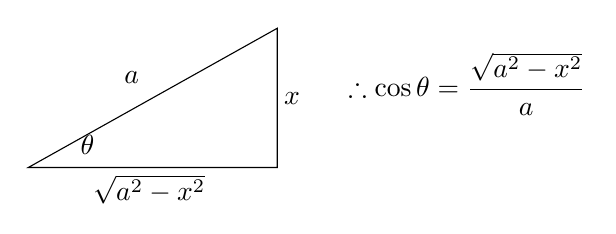
\begin{tikzpicture}[x=0.75pt,y=0.75pt,yscale=-1,xscale=1]
		\draw (223,191.88) -- (103,259) -- (223,259) -- cycle ;
		\draw (127,242.4) node [anchor=north west][inner sep=0.75pt]    {$\theta $};
		\draw (148,211.4) node [anchor=north west][inner sep=0.75pt]    {$\mathnormal{a}$};
		\draw (225,221.4) node [anchor=north west][inner sep=0.75pt]    {$x$};
		\draw (133,261.4) node [anchor=north west][inner sep=0.75pt]    {$\sqrt{a^{2} -x^{2}}$};
		\draw (256,202.4) node [anchor=north west][inner sep=0.75pt]    {$\therefore \cos \theta =\dfrac{\sqrt{a^{2} -x^{2}}}{a}$};
	\end{tikzpicture}
	$$\begin{aligned}
		\therefore\int\sqrt{a^2-x^2}\ \d x&=\frac{a^2}{2}(\theta+\sin\theta\cos\theta)+C\\
		&=\frac{a^2}{2}\left(\sin^{-1}\frac{x}{a}+\frac{x\sqrt{a^2-x^2}}{a^2}\right)+C
	\end{aligned}$$
\end{eg}
\begin{thm}{Table of Trigonometric Substitutions}
	\begin{tabular}{c|c|c}
		\textbf{Expression} & \textbf{Substitution}                                                                & \textbf{Identity}             \\
		$\sqrt{a^2-x^2}$    & $x=a\sin\theta,\ -\dfrac{\pi}{2}\leq\theta\leq\dfrac{\pi}{2}$                        & $1-\sin^2\theta=\cos^2\theta$ \\
		\text{ }&\text{ }&\text{ }\\
		$\sqrt{a^2+x^2}$    & $x=a\tan\theta,\ -\dfrac{\pi}{2}<\theta<\dfrac{\pi}{2}$                               & $1+\tan^2\theta=\sec^2\theta$ \\
		\text{ }&\text{ }&\text{ }\\
		$\sqrt{x^2-a^2}$    & $x=a\sec\theta,\ 0\leq\theta<\dfrac{\pi}{2}\text{ or }\pi\leq\theta<\dfrac{3\pi}{2}$ & $\sec^2\theta-1=\tan^2\theta$
	\end{tabular}
\end{thm}
\begin{eg}{Example 3}
	$$\int\frac{1}{x^2\sqrt{x^2+4}}\ \d x$$
	\noindent\rule[0.25\baselineskip]{\textwidth}{1pt}
	Let $x=2\tan\theta$, so we have $\d x=2\sec^2\theta\ \d\theta$: 
	$$\begin{aligned}
		\therefore\int\frac{1}{x^2\sqrt{x^2+4}}\ \d x&=\int\frac{1}{4\tan^2\theta\sqrt{4\tan^2\theta+4}}\cdot 2\sec^2\theta\ \d \theta\\
		&=\int\frac{1}{4\tan^2\theta\sqrt{4\left(\tan^2\theta+1\right)}}\cdot 2\sec^2\theta\ \d \theta\\
		&=\int\frac{1}{4\tan^2\theta\sqrt{4\sec^2\theta}}\cdot 2\sec^2\theta\ \d \theta\\
		&=\int\frac{1}{4\tan^2\theta\cdot 2\sec\theta}\cdot 2\sec^2\theta\ \d \theta\\
		&=\frac{1}{4}\int\frac{\sec\theta}{\tan^2\theta}\ \d \theta\\
		&=\frac{1}{4}\int\frac{\ \ \dfrac{1}{\cos\theta}\ \ }{\ \ \dfrac{\sin^2\theta}{\cos^2\theta}\ \ }\ \d \theta\\
		&=\frac{1}{4}\int\frac{\cos^2\theta}{\cos\theta\sin^2\theta}\ \d \theta\\
		&=\frac{1}{4}\int\frac{\cos\theta}{\sin^2\theta}\ \d \theta\\
	\end{aligned}$$
	Let $u=\sin\theta,\ \d u=\cos\theta\ \d\theta$: 
	$$\begin{aligned}
		\therefore\int\frac{1}{x^2\sqrt{x^2+4}}\ \d x&=\frac{1}{4}\int\frac{1}{u^2}\ \d u=\frac{1}{4}\int u^{-2}\ \d u\\
		&=-\frac{1}{4}u^{-1}+C=-\frac{1}{4u}+C\\
		&=-\frac{1}{4\sin\theta}+C
	\end{aligned}$$
	We need to go back in terms of $x$: \\
	$x=2\tan\theta\ \Rightarrow\ \tan\theta=\dfrac{x}{2}$\\
	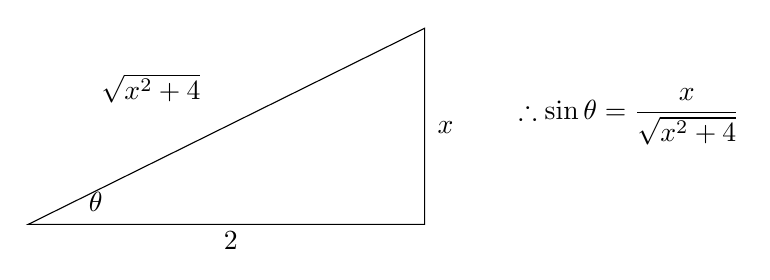
\begin{tikzpicture}[x=0.75pt,y=0.75pt,yscale=-1,xscale=1]
		\draw   (361,71.5) -- (170,166) -- (361,166) -- cycle ;
		\draw (204,92.4) node [anchor=north west][inner sep=0.75pt]    {$\sqrt{x^{2} +4}$};
		\draw (366,115.4) node [anchor=north west][inner sep=0.75pt]    {$x$};
		\draw (263,168.4) node [anchor=north west][inner sep=0.75pt]    {$2$};
		\draw (198,149.4) node [anchor=north west][inner sep=0.75pt]    {$\theta $};
		\draw (405,99.4) node [anchor=north west][inner sep=0.75pt]    {$\therefore \sin \theta =\dfrac{x}{\sqrt{x^{2} +4}}$};
	\end{tikzpicture}
	$$\begin{aligned}
		\therefore\int\frac{1}{x^2\sqrt{x^2+4}}\ \d x&=-\frac{1}{4\sin\theta}+C\\
		&=-\frac{\sqrt{x^2+4}}{4x}+C
	\end{aligned}$$
\end{eg}
\begin{eg}{Example 4}
	$$\int\frac{\d x}{\sqrt{x^2-a^2}},\text{ where }a>0$$
	\noindent\rule[0.25\baselineskip]{\textwidth}{1pt}
	Let $x=a\sec\theta$, then we have $\d x=a\sec\theta\tan\theta\ \d\theta$: 
	$$\begin{aligned}
		\therefore\int\frac{\d x}{\sqrt{x^2-a^2}}&=\int\frac{a\sec\theta\tan\theta\ \d\theta}{\sqrt{a^2\sec^2\theta-a^2}}\\
		&=\int\frac{a\sec\theta\tan\theta\ \d\theta}{\sqrt{a^2\left(\sec^2\theta-1\right)}}\\
		&=\int\frac{a\sec\theta\tan\theta\ \d\theta}{\sqrt{a^2\tan^2\theta}}\\
		&=\int\frac{a\sec\theta\tan\theta}{a\tan\theta}\ \d\theta\\
		&=\int\sec\theta\ \d\theta\\
		&=\ln\left|\tan\theta+\sec\theta\right|+C
	\end{aligned}$$
	Now, we want the answer in terms of $x$: \\
	$x=a\sec\theta\ \Rightarrow\ \sec\theta=\dfrac{x}{a},\ \cos\theta=\dfrac{a}{x}$. Using a right angle triangle, we can find $tan\theta$: 
	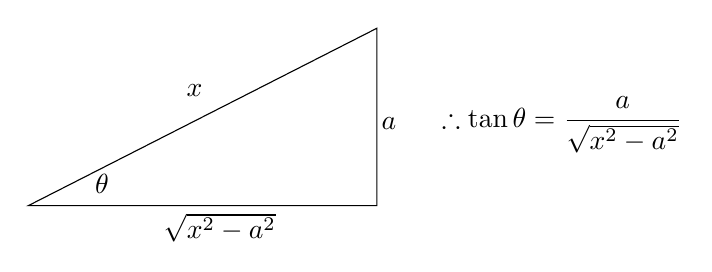
\begin{tikzpicture}[x=0.75pt,y=0.75pt,yscale=-1,xscale=1]
		\draw   (265,47.5) -- (97,133) -- (265,133) -- cycle ;
		\draw (128,116.4) node [anchor=north west][inner sep=0.75pt]    {$\theta $};
		\draw (172,73.4) node [anchor=north west][inner sep=0.75pt]    {$x$};
		\draw (266,89.4) node [anchor=north west][inner sep=0.75pt]    {$a$};
		\draw (161,135.4) node [anchor=north west][inner sep=0.75pt]    {$\sqrt{x^{2} -a^{2}}$};
		\draw (295,79.4) node [anchor=north west][inner sep=0.75pt]    {$\therefore \tan \theta =\dfrac{a}{\sqrt{x^{2} -a^{2}}}$};
	\end{tikzpicture}
	$$\therefore\int\frac{\d x}{\sqrt{x^2-a^2}}=\ln\left|\frac{a}{\sqrt{x^2-a^2}+\frac{x}{a}}\right|+C$$
\end{eg}

\subsection{Partial Fractions}
Recall that we know how to find common denominators: 
$$\frac{1}{x-1}-\frac{1}{x+1}=\frac{x+1-x+1}{(x-1)(x+1)}=\frac{2}{x^2-1}$$
Now, let's compare which side of the equation, the left-hand side or the right-hand side, is easier to integrate. The answer is the left handed side is easier to integrate: 
$$\begin{aligned}
	\int\left(\frac{1}{x-1}-\frac{1}{x+1}\right)\ \d x&=\int\frac{1}{x-1}\ \d x-\int\frac{1}{x+1}\ \d x\\
	&=\ln\left|x-1\right|-\ln\left|x+1\right|+C\\
	&=\ln\left|\frac{x-1}{x+1}\right|+C
\end{aligned}$$
\begin{eg}{The Goal of Partial Fractions}
	Given something like $\dfrac{2}{x^2-1}$, ``undo" the common denominator. That is, if possible, find constants $A$ and $B$ such that
	$$\frac{2}{(x-1)(x+2)}=\frac{A}{x-1}+\frac{B}{x+1}$$
	Then, 
	$$\int\frac{2}{x^2-1}\ \d x = \int\frac{2}{(x-1)(x+2)}\ \d x = \int\frac{A}{x-1}\ \d x+\int\frac{B}{x+1}\ \d x$$
\end{eg}
\begin{thm}{Basic Idea of Partial Fraction Decomposition}
	\textbf{Given}: a rational function, $f(x)=\dfrac{P(x)}{Q(x)}$, where $P(x)$ and $Q(x)$ are polynomials with degree$(P(x))<$degree$(Q(x))$.\\
	\textbf{Goal}: write $f(x)$ as $$f(x)=\frac{P(x)}{Q(x)}=F_1+F_2+\cdots+F_k,$$where each $F_i$ looks like $\dfrac{A}{(ax+b)^n}$ or $\dfrac{Ax+B}{(ax^2+bx+c)^n}$
\end{thm}
\begin{thm}{Approach to get Partial Fraction Decomposition}
	\begin{enumerate}
		\item If degree$(P(x))\geq$degree$(Q(x))$, use long division to get $$\text{polynomial}+\frac{\text{new }P(x)}{\text{new }Q(x)}$$
		\item Factorize $Q(x)$ as much as possible to get terms like \\ $$\begin{aligned}&(ax+b)^n\text{ (linear terms)}\\&(ax^2+bx+c)^n\text{( irreducible quadratic terms)}\end{aligned}$$
		\item For each $(ax+b)^n$, the decomposition contains: $$\frac{A_1}{(ax+b)}+\frac{A_2}{(ax+b)^2}+\cdots+\frac{A_n}{(ax+b)^n}$$For each irreducible quadratic $(ax^2+b x+c)^n$, the decomposition contains: $$\frac{Ax_1+B_1}{(ax^2+bx+c)}+\frac{Ax_2+B_2}{(ax^2+bx+c)^2}+\cdots+\frac{Ax_n+B_n}{(ax^2+bx+c)^n}$$
		\item Use algebra to find all $A_i$ and $B_i$
	\end{enumerate}
\end{thm}
\begin{eg}{Example 1}
	$$\int\frac{x^3-6x^2+5x-3}{x^2-1}\ \d x$$
	\noindent\rule[0.25\baselineskip]{\textwidth}{1pt}
	Because degree(numerator)$>$degree(denominator), we need to run a long division
	$$\begin{array}{lr} 
		& x-6 \\ 
		x^2+0-1  \!\!\!\!\!\! & \overline{)x^3-6x^2+5x-31} \\ 
		& \underline{x^3+\ 0x^2- \ \ x \ \ \ \ \ \ \ \ } \\ 
		& -6x^2+6x-\ \ 3 \\
		& \underline{-6x^2-0x+\ \ 6} \\ 
		& 6x-9 
	\end{array}$$
	$$\begin{aligned}
		\therefore \frac{x^3-6x^2+5x-3}{x^2-1}&=\frac{(x-6)(x^2-1)+(6x-9)}{x^2-1}\\
		&=(x-6)+\frac{6x-9}{x^2-1}
	\end{aligned}$$
	Factorize the denominator: 
	$$(x-6)-\frac{6x-9}{x^2-1}=(x-6)-\frac{6x-9}{(x-1)(x+1)}$$
	Partial fraction decomposition: \\
	$$\frac{6x-9}{(x-1)(x+2)}=\frac{A}{x-1}+\frac{B}{x+1}$$
	Find $A$ and $B$: 
	$$\frac{A}{x-1}+\frac{B}{x+1}=\frac{A(x+1)+B(x-1)}{(x-1)(x+1)}=\frac{6x-9}{(x-1)(x+1)}$$
	\quad $\boxed{\text{Method 1}}$ Solving system of equation: 
	$$\therefore\begin{cases}
		(A+B)x=6x\\
		A-B=-9
	\end{cases}\ \Rightarrow\ \begin{cases}
		A+B=6\\
		A-B=-9
	\end{cases}\ \Rightarrow\ \begin{cases}
		A=-3/2\\
		B=15/2
	\end{cases}$$
	\quad $\boxed{\text{Method 2}}$ Plug-in roots (Does not always apply)
	$$A(x+1)+B(x-1)=6x-9$$
	\quad\quad Let $x=1$: $$A(1+1)+B(1-1)=6(1)-9\ \Rightarrow\ 2A=6-9=-3$$ 
	$$\therefore A=-\frac{3}{2}$$
	\quad\quad Let $x=-1$: $$A(-1+1)+B(-1-1)=6(-1)-9\ \Rightarrow\ -2B=-6-9=-15$$
	$$\therefore B=\frac{15}{2}$$
	$$\therefore \frac{6x-9}{(x-1)(x+2)}=-\frac{3}{2}\cdot\frac{1}{x-1}+\frac{15}{2}\cdot\frac{1}{x+1}$$
	Find the integral: 
	$$\begin{aligned}
		\therefore\int\frac{x^3-6x^2+5x-3}{x^2-1}\ \d x&=\int(x-6)+\left(-\frac{3}{2}\cdot\frac{1}{x-1}+\frac{15}{2}\cdot\frac{1}{x+1}\right)\ \d x\\
		&=\int(x-6)\ \d x-\frac{3}{2}\int\frac{1}{x-1}\ \d x+\frac{15}{2}\int\frac{1}{x+1}\ \d x\\
		&=\frac{1}{2}x^2-6x-\frac{3}{2}\ln|x-1|+\frac{15}{2}\ln|x+1|+C
	\end{aligned}$$
\end{eg}
\begin{eg}{Example 2}
	$$\int\frac{x+2}{(x^2+2x+1)(x-1)}\ \d x$$
	\noindent\rule[0.25\baselineskip]{\textwidth}{1pt}
	Because degree(numerator)$<$degree(denominator): Nothing to do here.\\
	Factorization:
	$$\frac{x+2}{(x^2+2x+1)(x-1)}=\frac{x+2}{(x+1)^2(x-1)}$$
	Decomposition: 
	$$\frac{x+2}{(x+1)^2(x-1)}=\frac{A}{x+1}+\frac{B}{(x+1)^2}+\frac{C}{x-1}$$
	Find $A,\ B,\ C$: 
	Start by Substituting roots: 
	$$x+2=A(x+1)(x-2)+B(x-1)+C(x+1)^2$$
	\quad Let $x=1$: $$1+2=A(1+1)(1-1)+B(1-1)+C(1+1)^2\ \Rightarrow\ 3=0\cdot A+0\cdot B+4\cdot C$$
	$$\therefore C=\frac{3}{4}$$
	\quad Let $x=-1$: $$-1+2=A(-1+1)(-1-1)+B(-1-1)+C(-1+1)^2\ \Rightarrow\ 1=0\cdot A-2B+0\cdot C$$
	$$\therefore B=-\frac{1}{2}$$
	\quad To find $A$, we need another equation that does not cancel the $A$ term. Let's try some numbers other than the roots: \par
	\quad Let $x=0$: $$0+2=A(0+1)(0-1)+B(0-1)+C(0+1)^2\ \Rightarrow\ 2=-A-B+C$$
	$$\therefore A=-\left(-\frac{1}{2}\right)+\frac{3}{4}-2=\frac{2+3-8}{4}=-\frac{3}{4}$$
	$$\therefore\int\frac{x+2}{(x^2+2x+1)(x-1)}=-\frac{3}{4}\cdot\frac{1}{x+1}+\left(-\frac{1}{2}\right)\cdot\frac{1}{(x+1)^2}+\frac{3}{4}\cdot\frac{1}{x-1}$$
	Integration: 
	$$\begin{aligned}
		\therefore\int\frac{x+2}{(x^2+2x+1)(x-1)}\ \d x&=\int-\frac{3}{4}\cdot\frac{1}{x+1}+\left(-\frac{1}{2}\right)\cdot\frac{1}{(x+1)^2}+\frac{3}{4}\cdot\frac{1}{x-1}\ \d x\\
		&=-\frac{3}{4}\int\frac{1}{x+1}\ \d x-\frac{1}{2}\int\frac{1}{(x+1)^2}\ \d x+\frac{3}{4}\int\frac{1}{x-1}\ \d x\\
		&=-\frac{3}{4}\ln|x+1|-\frac{1}{2}\int\frac{1}{(x+1)^2}\ \d x+\frac{3}{4}\ln|x-1|
	\end{aligned}$$
	To find $\displaystyle\int\frac{1}{(x+1)^2}$, use $u$-substitution: Let $u=x+1$, so we have $\d u=\d x$
	$$\begin{aligned}
		\therefore\int\frac{1}{(x+1)^2}\ \d x=&\int=frac{1}{u^2}\ \d u\\
		&=-u^{-1}\\
		&=-\frac{1}{x+1}
	\end{aligned}$$
	$$\begin{aligned}
		\therefore\int\frac{x+2}{(x^2+2x+1)(x-1)}\ \d x&=-\frac{3}{4}\ln|x+1|-\frac{1}{2}\cdot\left(-\frac{1}{x+1}\right)+\frac{3}{4}\ln|x-1|+C\\
		&=-\frac{3}{4}\ln|x+1+\frac{1}{2(x+1)}+\frac{3}{4}\ln|x-1|+C
	\end{aligned}$$
\end{eg}
\begin{eg}{Example 3}
	$$\int\frac{4x^3-3x^2+6x-27}{x^4+9x^2}\ \d x$$
	\noindent\rule[0.25\baselineskip]{\textwidth}{1pt}
	Because degree(numerator)<degree(denominator), nothing to do here.\\
	Factorization: 
	$$x^4+9x^2=x^2(x^2+9)$$
	\begin{rmk}{Terms in this Example}
		$x^2$ is a linear term, whereas $x^2+9$ is an irreducible quadratic term. 
	\end{rmk}
	Decomposition: 
	$$\frac{4x^3-3x^2+6x-27}{x^4+9x^2}=\frac{4x^3-3x^2+6x-27}{x^2(x^2+9)}=\frac{A}{x}+\frac{B}{x^2}+\frac{Cx+D}{x^2+9}$$
	Find $A,\ B,\ C,\ D$: 
	$$\begin{aligned}
		\therefore 4x^3-3x^2+6x-27&=Ax(x^2+9)+B(x^2+9)+(Cx+D)x^2\\
		&=Ax^3+9Ax+Bx^2+9B+Cx^3+Dx^2\\
		&=(A+C)x^3+(B+D)x^2+9Ax+9B
	\end{aligned}$$
	Matching the coefficient: 
	$$\begin{cases}
		A+C=4\\
		B+D=-3\\
		9A=6\\
		9B=-27
	\end{cases}\ \Rightarrow\ \begin{cases}
		A=2/3\\
		B=-3\\
		C=4-A=10/3\\
		D=-3-B=0
	\end{cases}$$
	$$\therefore\frac{4x^3-3x^2+6x-27}{x^2(x^2+9)}=\frac{2}{3}\cdot\frac{1}{x}-\frac{3}{x^2}+\frac{10}{3}\cdot\frac{x}{x^2+9}$$
	Integration: 
	$$\begin{aligned}
		\therefore\int\frac{4x^3-3x^2+6x-27}{x^4+9x^2}\ \d x&=\int\frac{2}{3}\cdot\frac{1}{x}-\frac{3}{x^2}+\frac{10}{3}\cdot\frac{x}{x^2+9}\ \d x\\
		&=\frac{2}{3}\int\frac{1}{x}\ \d x-3\int\frac{1}{x^2}\ \d x+\frac{10}{3}\int\frac{x}{x^2+9}\ \d x\\
		&=\frac{2}{3}\ln|x|-3(-1)\frac{1}{x}+\frac{10}{3}\int\frac{x}{x^2+9}\ \d x
	\end{aligned}$$
	Use $u$-substitution to find $\displaystyle\int\frac{x}{x^2+9}\ \d x$: Let $u=x^2+9$, we have $\dfrac{\d u}{\d x}=2x\ \Rightarrow\ \d u=2x\ \d x$
	$$\therefore\int\frac{x}{x^2+9}\ \d x=\frac{1}{2}\int\frac{1}{u}\ \d u=\frac{1}{2}\ln|u|=\frac{1}{2}\ln|x^2+9|$$
	$$\begin{aligned}
		\therefore\int\frac{4x^3-3x^2+6x-27}{x^4+9x^2}\ \d x&=\frac{2}{3}\ln|x|-3(-1)\frac{1}{x}+\frac{10}{3}\cdot\frac{1}{2}\ln|x^2+9|+C\\
		&=\frac{2}{3}\ln|x|+\frac{3}{x}+\frac{5}{3}\ln|x^2+9|+C
	\end{aligned}$$
\end{eg}

\subsection{Improper Integrals}\label{improper}
Before starting the discussion on improper integrals, we need to first define proper integrals.
\begin{df}{Proper Integrals}
	An integral $\displaystyle\int_a^bf(x)\ \d x$ is considered to be proper \textit{iff}: 
	\begin{enumerate}
		\item $\left[a, b\right]$ is a finite interval, and
		\item $f(x)$ is continuous on $\left[a, b\right]$.
	\end{enumerate}
	If either of the two properties is not satisfied, the integral is called \textbf{\textit{improper}}.
\end{df}
By examining the definition of proper integrals, we know there are two types of improper integrals. \textbf{Type I} improper integrals fail to satisfy the first condition, and is called \textbf{infinite intervals}; \textbf{Type II} improper integrals do not satisfy the second condition and is called \textbf{discontinuous integrals}.
\subsubsection{Type I Improper Integrals: Infinite Intervals}
\begin{thm}{General Procedure to Solve Type I improper Integrals}
	\begin{enumerate}
		\item To solve $\displaystyle\int_a^\infty f(x)\ \d x$, we go through the following procedure: \\
		If $\displaystyle\int_a^tf(x)\ \d x$ exists $\forall t\geq a$, then $$\int_a^\infty f(x)\ \d x=\lim_{t\to\infty}\int_a^tf(x)\ \d x.$$
		\item To solve $\displaystyle\int^b_{-\infty} f(x)\ \d x$, we go through the following procedure: \\
		If $\displaystyle\int^b_tf(x)\ \d x$ exists $\forall t\leq b$, then $$\int^b_{-\infty} f(x)\ \d x=\lim_{t\to-\infty}\int^b_tf(x)\ \d x.$$
		\item Provided the limits exist as finite numbers, we define the integral \textbf{converges}.
		\item If both $\displaystyle\int_a^\infty f(x)\ \d x$ and $\displaystyle\int^a_{-\infty} f(x)\ \d x$ are convergent, then we define: 
		$$\int_{-\infty}^\infty f(x)\ \d x=\int^a_{-\infty} f(x)\ \d x+\int_a^\infty f(x)\ \d x$$
	\end{enumerate}
\end{thm}
\begin{eg}{Example 1}
	$$\int_1^\infty\frac{1}{x}\ \d x$$
	\noindent\rule[0.25\baselineskip]{\textwidth}{1pt}
	$$\begin{aligned}
		\int_1^\infty\frac{1}{x}\ \d x&=\lim_{t\to\infty}\int_1^t\frac{1}{x}\ \d x\\
		&=\lim_{t\to\infty}\bigg[\ln|x|\bigg]^t_1\\
		&=\lim_{t\to\infty}\left(\ln(t)-\ln(1)\right)\\
		&=\lim_{t\to\infty}\ln(t)=\infty
	\end{aligned}$$
	$\therefore$ Since the limit D.N.E. as a finite number, $\displaystyle\int_1^\infty\frac{1}{x}\ \d x$ is divergent. 
\end{eg}
\begin{eg}{Example 2}
	$$\int_1^\infty\frac{1}{x^2}\ \d x$$
	\noindent\rule[0.25\baselineskip]{\textwidth}{1pt}
	$$\begin{aligned}
		\int_1^\infty\frac{1}{x^2}\ \d x&=\lim_{t\to\infty}\int_1^t\frac{1}{x^2}\ \d x\\
		&=\lim_{t\to\infty}\bigg[-\frac{1}{x}\bigg]^t_1\\
		&=\lim_{t\to\infty}\left(-\frac{1}{t}-(-1)\right)\\
		&=\lim_{t\to\infty}\left(-\frac{1}{t}+1\right)\\
		&=0+1=1
	\end{aligned}$$
	$\therefore$ Since the limit exists as a finite number, $\displaystyle\int_1^\infty\frac{1}{x^2}\ \d x$ is convergent. 
\end{eg}
\begin{ext}{Generalization}
	For what values of $p$ is the integral $\displaystyle\int_1^\infty\frac{1}{x^p}\ \d x$ convergent? \\
	\noindent\rule[0.25\baselineskip]{\textwidth}{1pt}
	We have already done $p=1$, in which we know the integral is divergent.\\
	So let's assume $p\neq 1$: 
	$$\begin{aligned}
		\int_1^\infty\frac{1}{x^p}\ \d x=\lim_{t\to\infty}\int_1^t\frac{1}{x^p}\ \d x&=\lim_{t\to\infty}\int_1^t x^{-p}\ \d x\\
		&=\lim_{t\to\infty}\bigg[\frac{1}{-p+1}\cdot x^{(-p+1)}\bigg]^t_1\\
		&=\lim_{t\to\infty}\left(\frac{1}{1-p}\cdot t^{(1-p)}-\frac{1}{1-p}\right)\\
		&=\lim_{t\to\infty}\frac{1}{1-p}\left(t^{(1-p)}-1\right)
	\end{aligned}$$
	\begin{itemize}
		\item If $p>1$, then $1-p<0$: we have $t^{(1-p)}\to0$ as $t\to\infty$.
		$$\therefore \int_1^\infty\frac{1}{x^p}\ \d x=\lim_{t\to\infty}\frac{1}{1-p}\left(t^{(1-p)}-1\right)=\frac{-1}{1-p}=\frac{1}{p-1}.$$
		As the limit exists as a finite number, the integral is convergent. 
		\item If $p<1$, then $1-p>0$: we have $t^{(1-p)}\to\infty$ as $t\to\infty$.
		$$\therefore \int_1^\infty\frac{1}{x^p}\ \d x=\lim_{t\to\infty}\frac{1}{1-p}\left(t^{(1-p)}-1\right)=\infty.$$
		Since the limit D.N.E. as a finite number, the integral is divergent. 
	\end{itemize}
\end{ext}
\begin{rmk}{Summary}
	$$\int_1^\infty\frac{1}{x^p}\ \d x\quad\text{is }\begin{cases}\text{ convergent if }\ &p>1\\\text{ divergent if }\ &p\leq1\end{cases}$$
\end{rmk}
\begin{eg}{Example 3}
	$$\int_{-\infty}^\infty\frac{1}{1+x^2}\ \d x$$
	\noindent\rule[0.25\baselineskip]{\textwidth}{1pt}
	$$\int_{-\infty}^\infty\frac{1}{1+x^2}\ \d x=\int_{-\infty}^0\frac{1}{1+x^2}\ \d x+\int_{0}^\infty\frac{1}{1+x^2}\ \d x.$$
	Note: We can do both of these separately, but in the case, the graph of $y=\dfrac{1}{1+x^2}$ is symmetric about the $y$-axis.
	$$\therefore \int_{-\infty}^0\frac{1}{1+x^2}\ \d x=\int_{0}^\infty\frac{1}{1+x^2}\ \d x$$
	To evaluate $\displaystyle\int_{0}^\infty\frac{1}{1+x^2}\ \d x$, recall the following properties: 
	\begin{enumerate}
		\item $$\int\frac{1}{1+x^2}\ \d x=\tan^{-1}{x}+C$$
		\item The graph of $t=\tan\theta$ and the graph of $t=\tan^{-1}\theta$.
		\item $$\tan^{-1}(0)=0; \theta\to\infty, \tan^{-1}\theta=\frac{\pi}{2}$$
	\end{enumerate}
	$$\begin{aligned}
		\therefore \int_{0}^\infty\frac{1}{1+x^2}\ \d x=\lim_{t\to\infty}\int_0^t\frac{1}{1+x^2}\ \d x&=\lim{t\to\infty}\bigg[\tan^{-1}x\bigg]^t_0\\
		&=\lim_{t\to\infty}\left(\tan^{-1}t-\tan^{-1}0\right)\\
		&=\frac{\pi}{2}-0\\
		&=\frac{\pi}{2}
	\end{aligned}$$
	Because the limit exists as a finite number, the integral is convergent. 
	$$\begin{aligned}
		\therefore\int_{-\infty}^\infty\frac{1}{1+x^2}\ \d x&=2\int_{0}^\infty\frac{1}{1+x^2}\ \d x\\
		&=2\cdot\frac{\pi}{2}\\
		&=\pi
	\end{aligned}$$
\end{eg}

\subsubsection{Type II improper Integrals: Discontinuous Integrals}
\begin{thm}{General Procedure to Solve Type II improper Integrals}
	\begin{enumerate}
		\item If $f$ is continuous on $[a, b)$ and discontinuous at $b$: 
		$$\int_a^bf(x)\ \d x=\boxed{\lim_{t\to b^-}\int_a^tf(x)\ \d x}$$
		Note: we only cares about the left side limit in the boxed formula. 
		\item If $f$ is continuous on $(a, b]$ and discontinuous at $a$: 
		$$\int_a^bf(x)\ \d x=\lim_{t\to a^+}\int_t^bf(x)\ \d x$$
		\item Provide the limit exists as finite numbers, the integral converges. 
		\item If $f$ is continuous on $[a, b]$ but has a discontinuity at $c$, where $a<c<b$, and if both $\displaystyle\int_a^cf(x)\ \d x$ and $\displaystyle\int_c^bf(x)\ \d x$ converges, then
		$$\int_a^bf(x)\ \d x = \int_a^cf(x)\ \d x+\int_c^bf(x)\ \d x$$
	\end{enumerate}
\end{thm}
\begin{eg}{Example 4}
	$$\int_2^5\frac{1}{\sqrt{x-2}}\ \d x$$
	\noindent\rule[0.25\baselineskip]{\textwidth}{1pt}
	It can be easily determined that this is a type II improper derivative because $$\begin{cases}x-2\geq0\\x-2\neq0\end{cases}\ \Rightarrow\ x>2.$$
	Hence, $f(x)=\dfrac{1}{\sqrt{x-2}}$ is not continuous at $x=2$.
	$$\begin{aligned}
		\therefore\int_2^5\frac{1}{x-2}\ \d x&=\lim_{t\to2^+}\int_t^5\frac{1}{\sqrt{x-2}}\ \d x\\
		&=\lim_{t\to2^+}\bigg[2\sqrt{x-2}\bigg]^5_t\\
		&=\lim_{t\to2^+}\left(2\sqrt{3}-2\sqrt{t-2}\right)\\
		&=2\sqrt{3}-0=2\sqrt{3}
	\end{aligned}$$
	Because the limit exists as a finite number, the integral is convergent. 
\end{eg}
\begin{eg}{Example 5}
	$$\int_0^3\frac{1}{x-1}\ \d x$$
	\noindent\rule[0.25\baselineskip]{\textwidth}{1pt}
	$f(x)=\dfrac{1}{x-1}$ is discontinuous at $x=1$.
	$$\therefore\int_0^3\frac{1}{x-1}\ \d x=\int_0^1\frac{1}{x-1}\ \d x+\int_1^3\frac{1}{x-1}\ \d x$$
	Evaluate $\displaystyle\int_0^1\frac{1}{x-1}\ \d x$: 
	$$\begin{aligned}
		\int_0^1\frac{1}{x-1}\ \d x&=\lim_{t\to1^-}\int_0^t\frac{1}{x-1}\ \d x\\
		&=\lim_{t\to1^-}\bigg[\ln|x-1|\bigg]^t_0\\
		&=\lim_{t\to1^-}\left(\ln|t-1|+\ln1\right)\\
		&=\ln|0|+0=-\infty
	\end{aligned}$$
	Because the limit D.N.E. as a finite number, the integral $\displaystyle\int_0^1\frac{1}{x-1}\ \d x$ diverges. \\
	Hence, $\displaystyle\int_0^3\frac{1}{x-1}\ \d x$ is also divergent. 
\end{eg}
\begin{thm}{Comparison Test for Improper Integrals}
	\textbf{Purpose}: Test to see if integral converges, without actually computing the result. \\
	\textbf{Procedure}: \\
	Suppose $f$ and $g$ are continuous functions with $f(x)\geq g(x)\ \ \forall x\geq a$. Then
	\begin{enumerate}
		\item If $\displaystyle\int_a^\infty f(x)\ \d x$ is convergent, then $\displaystyle\int_a^\infty g(x)\ \d x$ is also convergent. 
		\item If $\displaystyle\int_a^b g(x)\ \d x$ is divergent, then $\displaystyle\int_a^b f(x)\ \d x$ is also divergent. 
	\end{enumerate}
\end{thm}
\begin{eg}{Example 6}
	$$\int_1^\infty\frac{1+e^{-x}}{x}\ \d x$$
	\noindent\rule[0.25\baselineskip]{\textwidth}{1pt}
	$$\begin{aligned} 
		&\because e^{-x}>0\\
		&\therefore 1+e^{-x}>1\\
		&\therefore\frac{1+e^{-x}}{x}>\frac{1}{x}
	\end{aligned}$$
	As $\displaystyle\int_1^\infty\frac{1}{x}\ \d x$ is divergent, $\displaystyle\int_1^\infty\frac{1+e^{-x}}{x}\ \d x$ is also divergent. 
\end{eg}

\newpage
\section{Differential Equations}
\subsection{Introduction to Ordinary Differential Equations}
Physical quantities often change with time (e.g. population changes with time), or position. So we model how quantities change with derivatives (Rates of change).
\begin{df}{Ordinary Differential Equations (ODE)}
	An equation relating an unknown function of one variable to one or more of its derivatives. 
\end{df}
\begin{df}{Solutions of an ODE}
	A function that satisfies the ODE.
\end{df}
\begin{df}{Order of an ODE}
	The highest order derivative in the ODE.
\end{df}
\begin{eg}{Example}
	Consider the ODE: $x^2y''-3xy'+3y=4x^7$.\\
	\noindent\rule[0.25\baselineskip]{\textwidth}{1pt}
	Here, the variable is not explicitly stated, so we assume $y=y(x)$, $y'=\dfrac{\d y}{\d x}$, $y''=\dfrac{\d^2 y}{\d x^2}$.
	\begin{enumerate}
		\item Order of the ODE: order = 2 because $y''$ is the highest order derivative. 
		\item Verify that $y=\dfrac{1}{6}x^7+x+x^3$ is an solution of the ODE.\\ 
		\newline Substitute $y=\dfrac{1}{6}x^7+x+x^3$: 
		$$\begin{aligned}
			\therefore y'&=\frac{7}{6}x^6+1+3x^2\\
			y''&=7x^5+6
		\end{aligned}$$
		$$\begin{aligned}
			\therefore \text{LHS}=x^2y''-3x y'+3y&=x^2(7x^5+6)-3x(\frac{7}{6}x^6+1+3x^2)+3(\frac{1}{6}x^7+x+x^3)\\
			&=7x^7+6x^2-\frac{7}{2}x^6-3x-9x^3+\frac{1}{2}x^7+3x\\
			&=\left(7-\frac{7}{2}+\frac{1}{2}\right)x^7+(6-9+3)x^3+(3-3)x\\
			&=4x^7=\text{RHS}
		\end{aligned}$$
	\end{enumerate}
\end{eg}
In general, it can be difficult to find a solution with a given ODE. There's not one general method for all ODEs. 
\begin{eg}{The Learning Curve}
	One model: The more you know, the slower you learn more about the task. \\
	If $y(t)=$percentage of a task learned over time, then $\dfrac{\d y}{\d t}$ decreases as $y$ increases. \\
	Suppose we are told: rate a person learns = percentage of task not yet learned. Then we can derive this differential equation: $$\frac{\d y}{\d x}=100-y(t).$$
	Observations: 
	\begin{enumerate}
		\item $$\frac{\d y}{\d x}>0\ \Rightarrow\ 100-y(t)>0\ \Rightarrow\ y(t)<100$$ That is, as long as a person has not learned everything, the rate at which they are learning is $>0$.
		\item $$\frac{\d y}{\d x}<0\ \Rightarrow\ 100-y(t)<0\ \Rightarrow\ y(t)>100$$ This does not make sense in this application. How can a person know more than everything? 
		\item $$\frac{\d y}{\d x}=0\ \Rightarrow\ 100-y(t)=0\ \Rightarrow\ y(t)=100$$
	\end{enumerate}
	Note: $y(t)=100$ is a solution of the ODE. 
	\begin{prf}{Proof}
		$$y(t)=100\ \Rightarrow\ \frac{\d y}{\d t}=0$$
		$$\begin{aligned}
			\therefore \text{LHS}&=\frac{\d y}{\d t}=0\\
			\text{RHS}&=100-y(t)=100-100=0\\
			\therefore \text{LHS}=\text{RHS}
		\end{aligned}$$
	\end{prf}
	\begin{df}{Equilibrium Solutions}
		Constant solutions, like $y(t)=100$, are called \textbf{equilibrium solutions} to the ODEs. 
	\end{df}
	Show that $y(t)=100+Ce^{-t}$, where $C$ is a constant, are solutions of the ODE. 
	$$\begin{aligned}
		&y(t)=100+Ce^{-t}\ \Rightarrow\ \frac{\d y}{\d t}=0-Ce^{-t}\\
		\therefore\ &\text{LHS}=\frac{\d y}{\d t}=-Ce^{-t},\ \text{RHS}=100-y=100-\left(100+Ce^{-t}\right)=-Ce^{-t}\\
		\therefore\ &\text{LHS}=\text{RHS}\text{, i.e., }y=100+Ce^{-t}\text{ are solutions of the ODE. }
	\end{aligned}$$
	\begin{rmk}{Remark}
		\begin{itemize}
			\item $C$ is a constant that depends on an initial condition.
			\item An initial value problem (IVP) is an ODE with an initial condition. 
		\end{itemize}
	\end{rmk} 
	\begin{enumerate}
		\item Solve the IVP: $\dfrac{\d y}{\d t}=100-y,\ y(0)=0$\\
		We know the general solution of the ODE is $y(t)=100+Ce^{-t}$: \\
		$$y(0)=0\ \Rightarrow\ 100+Ce^0=0\ \Rightarrow\ C=-100$$
		$$\therefore y(t)=100-100e^{-t}.$$
		\item Solve the IVP: $\dfrac{\d y}{\d t}=100-y,\ y(0)=10$\\
		We know the general solution of the ODE is $y(t)=100+Ce^{-t}$: \\
		$$y(0)=10\ \Rightarrow\ 100+Ce^0=10\ \Rightarrow\ C=-90$$
		$$\therefore y(t)=100-90e^{-t}.$$
	\end{enumerate}
\end{eg}

\subsection{Direction Fields and Euler's Method to Solve ODEs}
Recall from Calculus I that the derivative of $y(x)$, $\dfrac{\d y}{\d x}$ is the slope of $y(x)$. 
\begin{thm}{Derivative as Slope}
	If $\dfrac{\d y}{\d x}=F(x, y)$, then $F(x,y)$ is the slope of $y(x)$ at the point $(x,y)$. As a result, $F(x,y)$ gives the direction of $y(x)$ at the point $(x,y)$.
\end{thm}
This theorem leads to our understanding of the direction fields. Basically, we draw a short line representing the direction of the function pointing to at a certain point on a grid. 
\begin{df}{Direction Fields (Slope Fields)}
	Draw small lines indicating slope for a bunch of points.
\end{df}
The \textbf{Euler's Method} is a crude way to approximate solutions of ODEs. The basic idea is the following: 
\begin{itemize}
	\item Think of direction field as a set of sign posts that point in certain directions. 
	\item Pick a starting point (initial condition)
	\item Take a small step in direction indicated by the slope. 
	\item Stop at a nearby point, and calculate a new slope. 
	\item Take a small step in direction indicated by the slope. 
\end{itemize} 
A detailed version of the Euler's Method: Assume $\dfrac{\d y}{\d x}=F(x,y)$ - 
\begin{itemize}
	\item Start at $(x_0, y_0)$ (This is the initial condition)
	\item Slope is $F(x,y)$
	\item Choose a new $x_1=x_0+h$
	\item We need to find $y$. To do this, we use slopes: 
	$$\frac{y_1-y_0}{x_1-x_0}=F(x_0,y_0)$$
	$$\begin{aligned}
		y_1&=y_0+(x_1-x_0)F(x_0,y_0)\\
		&=y_0+(x_0+h-x_0)F(x_0,y_0)\\
		&=y_0+h\cdot F(x_0,y_0)
	\end{aligned}$$
	\item New slope: $F(x_1,y_1)$
	\item Choose new $x_2=x_1+h$
	\item Find $y_2$, using slopes: 
	$$\frac{y_2-y_1}{x_2-x_1}=F(x_1,y_1)$$
	$$y_2=y_1+h\cdot F(x_1,y_1)$$
\end{itemize}
\begin{thm}{The Euler's Method}
	\begin{itemize}
		\item Given an IVP: $\dfrac{\d y}{\d x}=F(x,y)$. $y(x_0)=y_0$
		\item Generate points: 
		$$\begin{aligned}
			x_1=x_0+h\quad\qquad&\quad\qquad y_1=y_0+hF(x_0,y_0)\\
			x_2=x_1+h\quad\qquad&\quad\qquad y_2=y_1+hF(x_1,y_1)\\
			x_3=x_2+h\quad\qquad&\quad\qquad y_3=y_2+hF(x_2,y_2)\\
			\ \ \vdots\quad\qquad\qquad&\qquad\qquad\qquad\vdots
		\end{aligned}$$
		where $h$ is a small number. 
		\item The curve through the points $(x_i,y_i)$ is an approximate solution of $y(x)$ of the IVP. 
	\end{itemize}
\end{thm}
\begin{eg}{Example}
	Consider the IVP: $\dfrac{\d y}{\d x}=-\dfrac{x}{y}$, $y(0)=1$\\
	Use Euler's method to approximate $y(0.3)$ with $h=0.1$.\\
	\noindent\rule[0.25\baselineskip]{\textwidth}{1pt}
	\begin{center}
		\begin{tabular}{c|c|c|c|c}
		$n$ & $x_n$ & $y_n$ & $\d y/\d x$ & $y_n+1$ \\ \hline
		$0$ & $0$ & $1$ & $0$ & $1+0.1\times0=1$ \\
		$1$ & $0.1$ & $1$ & $-0.1$ & $1-0.1\times 0.1=0.99$ \\
		$2$ & $0.2$ & $0.99$ & $-0.202$ & $0.99-0.1\times0.202=0.9698$ \\
		$3$ & $0.3$ & $0.9698$ & $\quad$  & $\quad$
		\end{tabular}
	\end{center}
\end{eg}

\subsection{Separate Variables to Solve ODEs}\label{Separate}
In this section, we will consider techniques to solve ODEs with the following form: 
$$\frac{\d y}{\ x}=F(x,y)=\boxed{g(x)f(y)}.$$
We can separate $F(x,y)$ as a product of: 
\begin{itemize}
	\item $g(x)$: a function only of $x$.
	\item $f(x)$: a function only of $y$.
\end{itemize}
To solve, move $x$-stuff to one side and $y$-stuff to the other side. Then, integrate. 
$$\Rightarrow \int\frac{1}{f(y)}\ \d y=\int g(x)\ \d x,\ f(y)\neq 0.$$ 
\begin{ext}{Notes on the Process}
	\begin{itemize}
		\item To do this, we need to assume $f(y)\neq 0$. 
		\item If $y=a$ is a constant such that $f(a)=0$, then $y=a$ is a valid solution to the ODE. 
		\begin{prf}{Proof}
			$$\begin{aligned}
				&y=a\ \Rightarrow\ \frac{\d y}{\d x}=0\\
				\therefore\ &\text{LHS}=\frac{\d y}{\d x}=0;\ \text{RHS}=f(a)g(x)=0\cdot g(x)=0\\
				\therefore\ &\text{LHS}=\text{RHS,\ i.e.,\ a solution to the ODE.}
			\end{aligned}$$
		\end{prf}
	\end{itemize}
\end{ext}
\begin{thm}{Separate Variables to Solve ODEs}
	To solve \textbf{\textit{separable}} ODEs, $\dfrac{\d y}{\d x}=g(x)f(y)$: 
	\begin{itemize}
		\item Solve $\displaystyle\int\frac{1}{f(y)}\ \d y=\int g(x)\ \d x$.
		\item Find constants $y=a$ where $f(a)=0$ (these are also solutions).
	\end{itemize}
\end{thm}
\begin{eg}{Example 1}
	Solve $\dfrac{\d y}{\d x}=-\dfrac{x}{y}$, $y(0)=1$.\\
	\noindent\rule[0.25\baselineskip]{\textwidth}{1pt}
	$$\begin{aligned}
		\int y\ \d y&=\int-x\ \d x\\
		\frac{1}{2}y^2&=-\frac{1}{2}x^2+C\\
		y^2&=-x^2+C
	\end{aligned}$$
	Substitute $x=0,\ y=1$: 
	$$1=-0+C\ \Rightarrow\ C=1$$
	$$\therefore y^2=-x^2+1\ \Rightarrow\ x^2+y^2=1.$$
\end{eg}
\begin{eg}{Example 2}
	Solve $\dfrac{\d y}{\d x}=x^2y^2$\\
	\noindent\rule[0.25\baselineskip]{\textwidth}{1pt}
	$$\begin{aligned}
		\int\frac{1}{y^2}\ \d y&=\int x^2\ \d x,\ y^2\neq 0\ \Rightarrow\ y\neq 0\\
		\int y^{-2}\ \d y&=\int x^2\ \d x\\
		-y^{-1}&=\frac{1}{3}x^3+C\\
		-\frac{1}{y}&=\frac{1}{3}x^3+C\\
		y&=-\frac{1}{\frac{1}{3}x^3+C}
	\end{aligned}$$
	$$\therefore\text{ all solutions are: }y=-\frac{1}{\frac{1}{3}x^3+C}\text{ and }y=0$$
\end{eg}
\begin{eg}{Example 3}
	Sometimes, we need to be creative. 
	Solve the following ODE: 
	$$\dfrac{\d y}{\d x}=xy-2y+x-2.$$
	\noindent\rule[0.25\baselineskip]{\textwidth}{1pt}
	$$\begin{aligned}
		\frac{\d y}{\d x}&=y(x-2)+(x-2)\\
		&=(x-2)(y+1)
	\end{aligned}$$
	Now, we can do the separation of variable easily: 
	$$\begin{aligned}
		\int\frac{1}{y+1}\ \d y&=\int(x-2)\ \d x,\ y+1\neq 0,\ y\neq-1\\
		\ln|y+1|&=\frac{1}{2}x^2-2x+C\\
		|y+1|&=e^{\frac{1}{2}x^2-2x+C}=e^{C}\cdot e^{\frac{1}{2}x^2-2x}\\
		y+1&=\pm\ e^{c}\cdot e^{\frac{1}{2}x^2-2x}\\
		y&=\pm\ A\cdot e^{\frac{1}{2}x^2-2x}, \\
		&\text{where }A\text{ can be any positive or negative constant; }A\text{ cannot be }0.
	\end{aligned}$$
	$$\therefore \text{All solutions are given by: }y=pm\ A\cdot e^{\frac{1}{2}x^2-2x}\text{ and }y=-1.$$
	Note: In this case, if we allow $A$ to also be $0$, we can write all solutions as $$y=\pm\ Ae^{\frac{1}{2}x^2-2x}-1.$$
\end{eg}
\begin{eg}{Example 4}
	\underline{Newton's Law of Cooling} states that the rate of change of temperature of an object is proportional to the difference between the temperature of the object and its surroundings. \\
	Set up and solve an ODE for this application. \\
	\noindent\rule[0.25\baselineskip]{\textwidth}{1pt}
	\begin{enumerate}
		\item Set up the ODE: \\
		Let $T(t)$ be the temperature of the object, $t$ is the time passed by, and $T_s$
		\item Solve the ODE: 
		$$\frac{\d T}{\d t}=-K(T-T_s)$$
		Assume $T_s$ is a constant (maybe a big assumption)
		$$\begin{aligned}
			\int\frac{1}{T-T_s}\ \d T&=\int-K\ \d t,\ T-T_s\neq 0(T\neq T_s)\\
			\ln|T-T_s|&=-Kt+C\\
			T-T_s&=e^{-Kt+C}=e^C\cdot e^{-Kt}=Ae^{-Kt}\\
			&\text{where }A\text{ can be any positive or negative constant.}
			T&=Ae^{-Kt}+T_s
		\end{aligned}$$
		$$\therefore \text{ All solutions are: }T=Ae^{-Kt}+T_s\text{ and }T=T_s$$
		If we allow $A$ to be $0$, we can write all solutions as $$T(t)=Ae^{-Kt}+T_s.$$
	\end{enumerate}
\end{eg}
\begin{eg}{Example 5}
	Solve the IVP: $$\frac{\d u}{\d t}=\frac{t(t^2+1)}{4u^3},\ u(0)=\frac{-1}{\sqrt{2}}.$$
	\noindent\rule[0.25\baselineskip]{\textwidth}{1pt}
	$$\begin{aligned}
		\int 4u^3\ \d u&=\int t^3+t\ \d t\\
		4\cdot\frac{1}{4}u^4=\frac{1}{4}t^5+\frac{1}{2}t^2+C\\
		u^4=\frac{1}{4}t^5+\frac{1}{2}t^2+C
	\end{aligned}$$
	Substitute $t=0,\ u=-\dfrac{1}{\sqrt{2}}$: 
	$$\left(-\dfrac{1}{\sqrt{2}}\right)^4=C\ \Rightarrow\ C=\frac{1}{4}$$
	$$\therefore u^4=\frac{1}{4}t^4+\frac{1}{2}t^2+\frac{1}{4}$$
	$$u=\sqrt[4]{\frac{1}{4}t^4+\frac{1}{2}t^2+\frac{1}{4}}.$$
\end{eg}

\subsection{ODE Models for Population Growth}
In this section, we consider some ODEs that are used to model population growth under certain assumptions. 
\begin{enumerate}
	\item Law of Natural Growth: \\
	Here we use the simple assumption that growth rate is proportional to population size. \\
	Let $P(t)=$Population size at any time $t$.\\
	Then $$\frac{\d P}{\d t}=k\cdot P.$$
	Note: $$\frac{1}{P}\cdot\frac{\d P}{\d t}=\frac{\d P/\d t}{P}=\frac{\text{Rate of growth}}{\text{population size}}=\text{``Relative growth rate"}$$
	$$\therefore k=\frac{1}{P}\frac{\d P}{\d t}=\text{Relative growth rate}.$$
	The OED: $\displaystyle\frac{\d P}{\d t}=kP$ is separable. 
	$$\begin{aligned}
		\int\frac{\d P}{P}&=\int k\ \d t\\
		\ln|P|&=kt+C\quad\Rightarrow\quad|P|=e^{kt+C}=e^C\cdot e^{kt}\\
		P&=\pm e^C\cdot e^{kt}=C_1e^{kt}
	\end{aligned}$$
	where $C_1$ is any positive or negative constant. 
	$$\therefore P=C_1e^{kt}\quad\text{and}\quad P=0.$$
	If we also allow $C_1$ to be 0, all solutions are $P(t)=C_1e^{kt}.$\\
	If $P(0)=P_0$, then $C_1\cdot e^{k\cdot 0}=P_0\quad\Rightarrow\quad C_1=P_0$
	\begin{thm}{Natural Growth ODE Model and Solution}
		$$\begin{aligned}
			\text{IVP: }&\quad\frac{\d P}{\d t}=kP,\ P(0)=P_0\\
			\text{Solution: }&\quad P(t)=P_0e^{kt}
		\end{aligned}$$	
	\end{thm}
	\begin{eg}{Example 1}
		Suppose: 
		\begin{itemize}
			\item Bacteria grows with constant relative growth rate, 
			\item count of bacteria was $400$ after $2$ hours, and
			\item count of bacteria was $25,600$ after $6$ hours. 	
		\end{itemize}
		How long did it take for the population to double $P_0$?
		\noindent\rule[0.25\baselineskip]{\textwidth}{1pt}
		From the first condition, we know the ODE above is applicable in this example. So we assume $\displaystyle\frac{\d P}{\d t}=kP$.\\
		From the second and the third condition, we get
		$$\begin{cases}
		P(2)=400\\P(6)=25600	
		\end{cases}
		\Longrightarrow
		\begin{cases}
		P_0e^{2k}=400&\qquad \mathrm{I}\\
		P_0e^{6k}=25600 &\qquad \mathrm{II}
		\end{cases}$$
		$$\begin{aligned}
			\frac{\mathrm{II}}{\mathrm{I}}:\ \frac{P_0e^{6k}}{P_0e^{2k}}&=\frac{25600}{400}\\
			e^{4k}&=64\\
			k&=\frac{1}{4}\ln(64)=\frac{1}{4}\ln(8^2)=\frac{1}{2}\ln(8)
		\end{aligned}$$
		We know $P(2)=400$: 
		$$\begin{aligned}
			\therefore P_0e^{2k}&=400\\
			P_0e^{2\cdot\frac{1}{2}\ln(8)}&=400\\
			P_0e^{\ln(8)}&=400\\
			8P_0&=400\\
			P_0=50\\
		\end{aligned}$$
		$$\begin{aligned}
			\therefore P(t)&=50e^{1/2\ln(8)t}\\
			&=50e^{t/2\ln(8)}\\
			&=50e^{\ln(8^{t/2})}\\
			&=50\cdot 8^{t/2}
		\end{aligned}$$
		So we need to find $t$ such that: 
		$$\begin{aligned}
			50\cdot 8^{t/2}&=100\\
			8^{t/2}&=2\\
			\ln(8^{t/2})&=\ln(2)\\
			\frac{t}{2}\ln(8)&=\ln(2)\\
			t&=2\cdot\frac{\ln(2)}{\ln(8)}=\frac{2\ln(2)}{\ln(2^3)}=\frac{2\ln(2)}{3\ln(2)}=\frac{2}{3}.
		\end{aligned}$$
	\end{eg}
	\item The Logistic Model:\\
	A more realistic model is that population growth should level off, and approach a ``carrying capacity" because of limited resources. \\
	\textbf{Assumptions}: 
	\begin{itemize}
		\item If $P$ is small, then $\displaystyle\frac{\d P}{\d t}\approx kP.$	
		\item As $P$ grows, the relative growth rate decreases as $P$ increases. 
		\item Relative growth rate should be negative if $P$ gets too large. \\
		That is 
		$$\frac{\d P}{\d t}>0\quad\text{for}\quad P<M$$
		$$\frac{\d P}{\d t}<0\quad\text{for}\quad P>M$$
		where $M$ is the ``carrying capacity" of $P$.
	\end{itemize}
	\textbf{An ODE model that incorporates these assumptions is}: 
	$$\frac{\d P}{\d t}=kP\left(1-\frac{P}{M}\right),\ k>0,\ M>0$$
	Notice: 
	$$P\approx0\quad\Rightarrow\quad\frac{P}{M}\approx0\quad\Rightarrow\quad\frac{\d P}{\d t}\approx kP$$
	$$P>M\quad\Rightarrow\quad\frac{P}{M}>1\quad\Rightarrow\quad\frac{\d P}{\d t}<0$$
	$$P<M\quad\Rightarrow\quad\frac{P}{M}<1\quad\Rightarrow\quad\frac{\d P}{\d t}>0$$
	\textbf{The equilibrium (constant) solutions are}: 
	$$\frac{\d P}{\d t}=0\ \Longrightarrow\ kP\left(1-\frac{P}{M}\right)=0\ \Rightarrow\ P=0\ \text{or}\ P=M.$$
	Note: This model does not take into account if the population is too small, then the population becomes extinct. \\
	\textbf{Finding all solutions of the OED}: 
	$$\frac{\d P}{\d t}=kP\left(1-\frac{P}{M}\right)$$
	$$\Rightarrow \frac{\d P}{P\left(1-\frac{P}{M}\right)}=k\ \d t,\ P\neq0,\ P\neq M$$
	Using partial fractions: 
	$$\frac{1}{P\left(1-\frac{P}{M}\right)}=\frac{M}{P(M-P)}=\frac{A}{P}+\frac{B}{M-P}$$
	$$\Rightarrow M=A(M-P)+B\cdot P$$
	$$P=0\ \Rightarrow\ M=A\cdot M\ \Rightarrow\ A=1$$
	$$P=M\ \Rightarrow\ M=B\cdot M\ \Rightarrow\ B=1$$
	$$\therefore \int \left[\frac{1}{P}+\frac{1}{M-P}\right]\ \d P=\int k\ \d t$$
	$$\begin{aligned}
		\ln|P|-\ln|M-P|&=kt+C_1\\
		\ln\left|\frac{P}{M-P}\right|&=kt+C_1\\
		\left|\frac{P}{M-P}\right|&=e^{kt+C_1}=e^{C_1}e^{kt}\\
		\frac{P}{M-P}&=\pm e^{C_1}\cdot e^{kt}\\
		&=Ce^{kt}
	\end{aligned}$$
	where $C$ can be any positive or negative constant. 
	Now, solve explicitly for $P$: 
	$$P=Ce^{kt}(M-P)=CMe^{kt}-Ce^{kt}P$$
	$$\begin{aligned}
		\left(1+Ce^{kt}\right)P&=CMe^{kt}\\
		P&=\frac{CMe^{kt}}{\left(1+Ce^{kt}\right)}\\
		&=\frac{CM}{e^{-kt}+C}\\
		&=\frac{M}{\frac{1}{C}e^{-kt}+1}=\frac{M}{Ae^{-kt}+1}\ \left(A=\frac{1}{C}\right)
	\end{aligned}$$
	Note: If $P(0)=P_0$, then
	$$\frac{M}{A+1}=P_0\ \Rightarrow\ \frac{M}{P_0}=A+1\ \Rightarrow A=\frac{M}{P_0}-1=\frac{M-P_0}{P_0}$$
	Therefore: $$P(t)=\frac{M}{\dfrac{M-P_0}{P_0}e^{-kt}+1}$$
	\begin{thm}{Logistic Growth ODE Model and Solution}
		Assume $M$ is the ``carrying capacity" of the population. 
		$$\begin{aligned}
			\text{IVP: }&\qquad\frac{\d P}{\d t}=kP\left(1-\frac{P}{M}\right),\ P(0)=P_0\\
			\text{General Solution: }&\qquad P(t)=\frac{M}{1+Ae^{-kt}},\ \text{where }A\text{ is a constant. }\\
			\text{If} P(0)=P_0,\ \text{then: }&\qquad A=\frac{M-P_0}{P_0}
		\end{aligned}$$	
	\end{thm}
	\textbf{When does the population grow fastest? }\\
	That is, when is $\displaystyle\frac{\d P}{\d t}$ maximized? i.e., we want to find when $\displaystyle\frac{\d}{\d t}\left(\frac{\d P}{\d t}\right)=0$.
	$$\begin{aligned}
		\frac{\d}{\d t}\left(\frac{\d P}{\d t}\right)&=\frac{\d}{\d t}\left(k-P\left(1-\frac{P}{M}\right)\right)\\
		&=kP'\left(1-\frac{P}{M}\right)+kP\left(0-\frac{P'}{M}\right)\\
		&=kP'\left(1-\frac{P}{M}-\frac{P}{M}\right)\\
		&kP'\left(1-\frac{2P}{M}\right)\qquad\left[\text{We know }P'=kP\left(1-\frac{P}{M}\right)\right]\\
		&=k^2\boxed{P\left(1-\frac{P}{M}\right)\left(1-\frac{2P}{M}\right)}
	\end{aligned}$$
	The boxed part will be $0$ if: 
	$$\begin{aligned}
		\text{minimum growth rate}&\qquad\begin{cases}P=0\\ P=M\end{cases}\\
		\text{maximum growth rate}&\qquad P=\frac{1}{2}M
	\end{aligned}$$
\end{enumerate}

\subsection{Linear Equations}
In section \ref{Separate}, we learned an approach to solve separable ODES. But what do we do if the ODE is not separable? The answer is that we need another approach. In this section, we consider an approach to solve \underline{\textbf{linear ODEs}}, which have the general equation: $$\frac{\d y}{\d x}+P(x)y=Q(x),$$where $P(x)$ and $Q(x)$ are functions of $x$.\\
We can derive an approach to solve this ODE:\\
Let $$\displaystyle I(x)=e^{\int P(x)\ \d x}$$ This is called the \underline{\textbf{integrating factor}}.\\
Note: $$\begin{aligned}
	\frac{\d}{\d x}\left[I(x)\right]&=\frac{\d}{\d x}\left[e^{\int P(x)\ \d x}\right]	\\
	&=e^{\int P(x)\ \d x}\cdot\frac{\d}{\d x}\\
	&=e^{\int P(x)\ \d x}\cdot P(x)\\
	&=I(x)P(x)\\
\therefore\frac{\d}{\d x}[I(x)]&=I(x)P(x)
\end{aligned}$$
Scale the ODE: 
$$\begin{aligned}
	\frac{\d y}{\d x}+P(x)&=Q(x)\\
	\boxed{I(x)\left[\frac{\d y}{\d x}+P(x)y\right]}&=I(x)Q(x)\\
\end{aligned}$$
By product rule: 
$$\begin{aligned}
	\frac{\d}{\d x}[I(x)y]&=\frac{\d}{\d x}[I(x)]y+I(x)\frac{\d y}{\d x}\\
	&=I(x)P(x)y+I(x)\frac{\d y}{\d x}\\
	&=\boxed{I(x)\left[P(x)y+\frac{\d y}{\d x}\right]}\\
	&I(x)Q(x)
\end{aligned}$$
$$\begin{aligned}
	\frac{\d}{\d x}[I(x)y]&=I(x)Q(x)\\
	\int\d[I(x)y]&=\int I(x)Q(x)\ \d x\\
	I(x)y&=	\int I(x)Q(x)\ \d x + C\\
	y&=\frac{1}{I(x)}\left[\int I(x)Q(x)\ \d x + C\right]
\end{aligned}$$
\textit{Note: Plus the constant before dividing $I(x)$ to both sides of the equation. }
\begin{thm}{Integrating Factor Method to Solve Linear ODEs}
	For linear ODEs: 
	$$\frac{\d y}{\d x}+P(x)y=Q(x): $$
	\begin{enumerate}
		\item Computing the integrating factor: $I(x)=e^{\int P(x)\ \d x}$ and simplify
		\item Set up the equation: $$I(x)y(x)=\underbrace{\int I(x)Q(x)\ \d x}_{\text{integrate and simplify}}$$
		\item Solve for $y$: $$y(x)=\frac{1}{I(x)}\left(\int I(x)Q(x)\ \d x+C\right)$$
	\end{enumerate}
\end{thm}
\begin{eg}{Example 1}
	Solve the ODE: $$xy'-4y=x^6e^x$$	
	\noindent\rule[0.25\baselineskip]{\textwidth}{1pt}
	The ODE is not in the standard form. 
	$$\frac{\d y}{\d x}-\frac{4}{x}y=x^5e^x\ \Rightarrow\ \therefore P(x)=-\frac{4}{x},\ Q(x)=x^5e^x$$
	$$\therefore I(x)=e^{\int P(x)\ \d x}=e^{-4\int\frac{1}{x}}\ \d x=e^{-4\ln{x}}=x^{-4}$$
	$$\begin{aligned}
		\therefore \frac{\d}{\d x}[I(x)y]&=I(x)Q(x)=x^{-4}x^5e^x=xe^x\\
		\int\d[I(x)y]&=\int xe^x\ \dx\\
		I(x)y&=\int xe^x\ \dx
	\end{aligned}$$
	Let $\begin{cases}u=x\\\d v=e^x \ \dx\end{cases}$, so we have $\begin{cases}\d u=\dx\\v=e^x\end{cases}$
	$$\begin{aligned}
		\therefore\int xe^x\ \dx&=xe^x-\int e^x\ \dx\\
		&=xe^x-e^x+C\\
		\therefore I(x)y&=xe^x-e^x+C\\
		x^{-4}y&=xe^x-e^x+C\\
		y&=x^5e^x-x^4e^x+Cx^4
	\end{aligned}$$
\end{eg}
\begin{eg}{Example 2}
	Solve the ODE: $$\dydx+2xy=x,\quad y(0)=-3.$$	
	\noindent\rule[0.25\baselineskip]{\textwidth}{1pt}
	$$P(x)=2x,\ Q(x)=x\ \Rightarrow\ I(x)=e^{\int P(x)\ \dx}=e^{\int 2x\ \dx}=e^{x^2}$$
	$$I(x)y=\int I(x)Q(x)\ \dx=\int e^{x^2}x\ \dx$$
	Let $u=x^2\ \Rightarrow\ \d u=2x\ \dx$
	$$\therefore\int e^{x^2}x\ \dx=\frac{1}{2}\int e^{u}\ 2x\dx=\frac{1}{2}\int e^u\ \d u=\frac{1}{2}e^u+C=\frac{1}{2}e^{x^2}+C$$
	$$\begin{aligned}
		\therefore e^{x^2}y&=\frac{1}{2}e^{x^2}+C\\
		y&=\frac{1}{2}+Ce^{-x^2}
	\end{aligned}$$
	Substitute $y(0)=3$: 
	$$\begin{aligned}
		-3&=\frac{1}{2}+Ce^0\\
		C&=-3-\frac{1}{2}=-\frac{7}{2}\\
		\therefore y&=\frac{1}{2}-\frac{7}{2}e^{-x^2}
	\end{aligned}$$
\end{eg}
\begin{eg}{Example 3}
	Solve the ODE: $$xy'+3y=x\ln(3+\cos^2x),\ x>0$$	
	\noindent\rule[0.25\baselineskip]{\textwidth}{1pt}	
	$$P(x)=\frac{3}{x},\ Q(x)=\ln(3+\cos^2x)\ \Rightarrow\ I(x)=e^{\int P(x)\ \dx}=e^{3\int\frac{1}{x}\ \dx}=e^{3\ln x}=x^3$$
	$$\begin{aligned}
		\therefore I(x)y&=\int I(x)Q(x)\ \dx\\
		x^3y&=\boxed{\int x^3\ln(3+\cos^2x)\ \dx}\\
		&\text{This is not easy to integrate.} \\
		&\text{Sometimes, we will stop here and write the solution as:}\\
		y&=\frac{1}{x^3}\left[\int x^3\ln(3+\cos^2x)\ \dx\right]
	\end{aligned}$$
\end{eg}
\begin{eg}{Example 4}
	Solve the ODE: $$xy'+y=-xy^2$$	
	\noindent\rule[0.25\baselineskip]{\textwidth}{1pt}
	Try to put it into the standard form: 
	$$\dydx+\frac{1}{x}y=-y^2$$
	However, this is still not in the standard form. \\
	In this case, we will  try substitution: 
	$$u=y^{-1}\ \Rightarrow\ y=u^{-1},\ y^2=u^{-2}$$
	$$\frac{\d u}{\d x}=-y^2\dydx\ \Rightarrow\ \dydx=-y^2\frac{\d u}{\d x}=-u^{-2}\frac{\d u}{\d x}$$
	$$\begin{aligned}
		-u^{-2}\frac{\d u}{\d x}+\frac{1}{x}u^{-1}&=-u^{-2}\\
		\frac{\d u}{\d x}-\frac{1}{x}u&=1
	\end{aligned}$$
	This is in the standard form: $\displaystyle P(x)=-\frac{1}{x},\ Q(x)=1$
	$$\therefore I(x)=e^{\int-\frac{1}{x}\ \dx}=e^{-\ln x}=x^{-1}$$
	$$\begin{aligned}
		\therefore I(x)u&=\int I(x)Q(x)\ \dx\\
		x^{-1}u&=\int x^{-1}\ \dx\\
		x^{-1}u&=\ln|x|+C\\
		u&=x\ln|x|+Cx\\
		\therefore y&=u^{-1}=\frac{1}{x\ln|x|+Cx}
	\end{aligned}$$
\end{eg}
\begin{thm}{General Approach of Substitution in Linear ODEs}
	If we have an ODE: $$\dydx+P(x)y=Q(x)y^n,$$where $n\neq 0,\ n\neq 1$	
	Then, use substitution: $$u=y^{1-n}$$
\end{thm}
\begin{eg}{Example 4 - \textit{Explained}}
	If $n=2$: $u=y^{1-2}=y^{-1}$
\end{eg}
\begin{ext}{Extension from the General Approach}
	If $n=1$: 
	$$\begin{aligned}
		\dydx+P(x)y&=Q(x)y\\
		\dydx+P(x)y-Q(x)y&=0\\
		\dydx+\left(P(x)-Q(x)\right)y=0
	\end{aligned}$$	
	This equation can be solved by separable variable or linear ODE.
	$$\begin{aligned}
		\boxed{\text{Separable}}\quad\dydx &=\left(Q(x)-P(x)\right)y\\
		\int\frac{1}{y}\ \d y&=\int Q(x)-P(x)\ \dx\\
		\boxed{\text{Linear ODE}}\quad I(x)&=e^{\int P(x)-Q(x)\ \dx}\\
	\end{aligned}$$
\end{ext}

\newpage
\section{Series}\label{series}
\subsection{Sequences}\label{sequence}
In section \ref{series}, we will study the very important topics of infinite sequences, and infinite series (i.e., adding an infinite sequence of numbers).

In section \ref{sequence}, we will introduce the concept of infinite sequences. 

\begin{df}{Sequence}
	A \textbf{sequence} is a function where the domain is \underline{the positive integers}.	
\end{df}
\begin{eg}{Example 1}
	Consider the sequence: $$a_n=\frac{10}{n}\ \Rightarrow\ \text{OR}\ f(n)=\frac{10}{n},\ n\in\Z^+.$$	
	\noindent\rule[0.25\baselineskip]{\textwidth}{1pt}
	$$\begin{aligned}
		a_1&=10\\
		a_2&=5\\
		&\vdots\\
		a_{10}&=1\\
		&\vdots\\
		a_{100}&=0.1\\
		&\vdots
	\end{aligned}$$
	Note: the trend of $a_n$ is growing to $0$.
\end{eg}
\begin{eg}{Example 2}
	Consider the sequence: $$a_n=(-1)^{n-1}n.$$	
	\noindent\rule[0.25\baselineskip]{\textwidth}{1pt}
	$$\begin{aligned}
		a_1&=1\\
		a_2&=-2\\
		a_3&=3\\
		a_{4}&=-4\\
		&\vdots
	\end{aligned}$$
	This is an alternating sign sequence. This sequence is alternating between larger and larger positive and negative numbers. 
\end{eg}
\begin{rmk}{Notations}
	Sequences are often written with brackets: 
	$$\left\{\frac{1}{n}\right\},\ \left\{(-1)^{n-1}n\right\},\ \left\{a_n\right\}.$$
\end{rmk}
An important question to answer in this section is that ``Does the sequence $\left\{a_n\right\}$ has a definite trend, or is it indecisive, as $n$ increases?" That is, does $\displaystyle\lim_{n\to\infty}a_n$ exist? If the limit exists, is it finite? 
$$\lim_{n\to\infty}a_n=L\quad\text{If }L\text{ is finite }\Rightarrow\text{ converges; otherwise, diverges.}$$
\begin{df}{Convergence of a Sequence}
	\begin{itemize}
	\item If $\displaystyle\lim_{n\to\infty}a_n=L$ (i.e., exists), we say the sequence $\left\{a_n\right\}$	\underline{converges} to $L$. 
	\item If $\displaystyle\lim_{n\to\infty}a_n=\pm\infty$ or does not exist ($\DNE$), we say the sequence $\left\{a_n\right\}$	\underline{diverges} to $L$. 
	\end{itemize}
\end{df}
\begin{df}{Formal Definition of Convergence}
	$\displaystyle\lim_{n\to\infty}a_n=L$ if for every (small) $\varepsilon>0$, there is an integer $n$ such that: 
	$$\boxed{\left|a_n-L\right|<\varepsilon}\ \text{whenever}\ n>N$$
	The boxed inequality stands for $-\varepsilon<a_n-L<\varepsilon$ (i.e., $L-\varepsilon<a_n<L+\varepsilon$).\\
	Note: $N$ depends on $\varepsilon$. If $\varepsilon$ is tiny, then $N$ may need to be large. \\
	But for $n>N$, $a_n$ will be in the envelope $L-\varepsilon$ and $L+\varepsilon$.
	\tikzset{every picture/.style={line width=0.75pt}}
	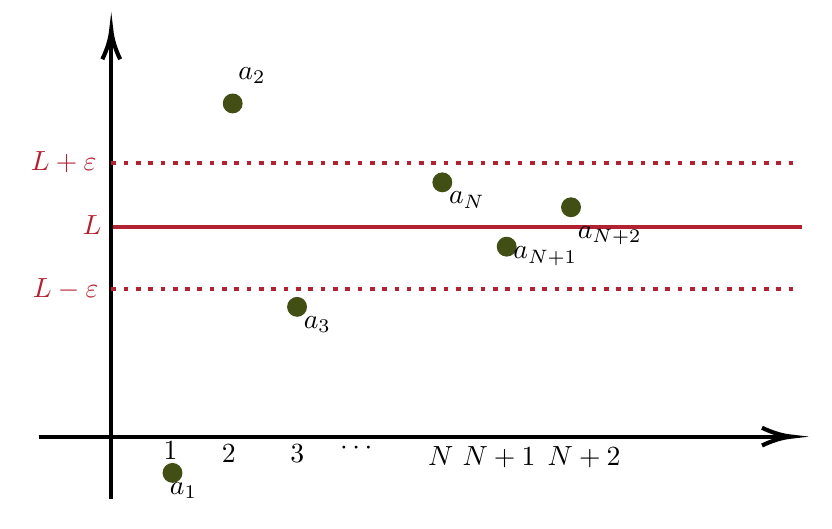
\begin{tikzpicture}[x=0.75pt,y=0.75pt,yscale=-1,xscale=1]
		\draw [line width=1.5]    (146,211) -- (505.74,211) ;
		\draw [shift={(508.74,211)}, rotate = 180] [color={rgb, 255:red, 0; green, 0; blue, 0 }  ][line width=1.5]    (14.21,-4.28) .. controls (9.04,-1.82) and (4.3,-0.39) .. (0,0) .. controls (4.3,0.39) and (9.04,1.82) .. (14.21,4.28)   ;
		\draw [line width=1.5]    (181,241) -- (181,17.97) ;
		\draw [shift={(181,14.97)}, rotate = 90] [color={rgb, 255:red, 0; green, 0; blue, 0 }  ][line width=1.5]    (14.21,-4.28) .. controls (9.04,-1.82) and (4.3,-0.39) .. (0,0) .. controls (4.3,0.39) and (9.04,1.82) .. (14.21,4.28)   ;
		\draw [color={rgb, 255:red, 208; green, 2; blue, 27 }  ,draw opacity=1 ][line width=1.5]  [dash pattern={on 1.69pt off 2.76pt}]  (181,79) -- (512.74,79) ;
		\draw [color={rgb, 255:red, 208; green, 2; blue, 27 }  ,draw opacity=1 ][line width=1.5]    (182,110) -- (513.74,110) ;
		\draw [color={rgb, 255:red, 208; green, 2; blue, 27 }  ,draw opacity=1 ][line width=1.5]  [dash pattern={on 1.69pt off 2.76pt}]  (181,140) -- (512.74,140) ;
		\draw  [color={rgb, 255:red, 74; green, 144; blue, 226 }  ,draw opacity=1 ][fill={rgb, 255:red, 74; green, 144; blue, 226 }  ,fill opacity=1 ] (206,228.49) .. controls (206,225.99) and (208.02,223.97) .. (210.51,223.97) .. controls (213.01,223.97) and (215.03,225.99) .. (215.03,228.49) .. controls (215.03,230.98) and (213.01,233) .. (210.51,233) .. controls (208.02,233) and (206,230.98) .. (206,228.49) -- cycle ;
		\draw  [color={rgb, 255:red, 74; green, 144; blue, 226 }  ,draw opacity=1 ][fill={rgb, 255:red, 74; green, 144; blue, 226 }  ,fill opacity=1 ] (235,50.49) .. controls (235,47.99) and (237.02,45.97) .. (239.51,45.97) .. controls (242.01,45.97) and (244.03,47.99) .. (244.03,50.49) .. controls (244.03,52.98) and (242.01,55) .. (239.51,55) .. controls (237.02,55) and (235,52.98) .. (235,50.49) -- cycle ;
		\draw  [color={rgb, 255:red, 74; green, 144; blue, 226 }  ,draw opacity=1 ][fill={rgb, 255:red, 74; green, 144; blue, 226 }  ,fill opacity=1 ] (266,148.49) .. controls (266,145.99) and (268.02,143.97) .. (270.51,143.97) .. controls (273.01,143.97) and (275.03,145.99) .. (275.03,148.49) .. controls (275.03,150.98) and (273.01,153) .. (270.51,153) .. controls (268.02,153) and (266,150.98) .. (266,148.49) -- cycle ;
		\draw  [color={rgb, 255:red, 74; green, 144; blue, 226 }  ,draw opacity=1 ][fill={rgb, 255:red, 74; green, 144; blue, 226 }  ,fill opacity=1 ] (336,88.49) .. controls (336,85.99) and (338.02,83.97) .. (340.51,83.97) .. controls (343.01,83.97) and (345.03,85.99) .. (345.03,88.49) .. controls (345.03,90.98) and (343.01,93) .. (340.51,93) .. controls (338.02,93) and (336,90.98) .. (336,88.49) -- cycle ;
		\draw  [color={rgb, 255:red, 74; green, 144; blue, 226 }  ,draw opacity=1 ][fill={rgb, 255:red, 74; green, 144; blue, 226 }  ,fill opacity=1 ] (367,119.49) .. controls (367,116.99) and (369.02,114.97) .. (371.51,114.97) .. controls (374.01,114.97) and (376.03,116.99) .. (376.03,119.49) .. controls (376.03,121.98) and (374.01,124) .. (371.51,124) .. controls (369.02,124) and (367,121.98) .. (367,119.49) -- cycle ;
		\draw  [color={rgb, 255:red, 74; green, 144; blue, 226 }  ,draw opacity=1 ][fill={rgb, 255:red, 74; green, 144; blue, 226 }  ,fill opacity=1 ] (398,100.49) .. controls (398,97.99) and (400.02,95.97) .. (402.51,95.97) .. controls (405.01,95.97) and (407.03,97.99) .. (407.03,100.49) .. controls (407.03,102.98) and (405.01,105) .. (402.51,105) .. controls (400.02,105) and (398,102.98) .. (398,100.49) -- cycle ;
		\draw (142,133.4) node [anchor=north west][inner sep=0.75pt]  [color={rgb, 255:red, 208; green, 2; blue, 27 }  ,opacity=1 ]  {$L-\varepsilon $};
		\draw (141,72.4) node [anchor=north west][inner sep=0.75pt]  [color={rgb, 255:red, 208; green, 2; blue, 27 }  ,opacity=1 ]  {$L+\varepsilon $};
		\draw (166,103.4) node [anchor=north west][inner sep=0.75pt]  [color={rgb, 255:red, 208; green, 2; blue, 27 }  ,opacity=1 ]  {$L$};
		\draw (205,212.4) node [anchor=north west][inner sep=0.75pt]    {$1$};
		\draw (233,213.4) node [anchor=north west][inner sep=0.75pt]    {$2$};
		\draw (266,213.4) node [anchor=north west][inner sep=0.75pt]    {$3$};
		\draw (332.37,214.4) node [anchor=north west][inner sep=0.75pt]    {$N$};
		\draw (349,214.4) node [anchor=north west][inner sep=0.75pt]    {$N+1$};
		\draw (390,214.4) node [anchor=north west][inner sep=0.75pt]    {$N+2$};
		\draw (208,231.89) node [anchor=north west][inner sep=0.75pt]    {$a_{1}$};
		\draw (241,31.89) node [anchor=north west][inner sep=0.75pt]    {$a_{2}$};
		\draw (272.51,151.89) node [anchor=north west][inner sep=0.75pt]    {$a_{3}$};
		\draw (342.51,91.89) node [anchor=north west][inner sep=0.75pt]    {$a_{N}$};
		\draw (373.51,118.37) node [anchor=north west][inner sep=0.75pt]    {$a_{N+1}$};
		\draw (404.51,108.4) node [anchor=north west][inner sep=0.75pt]    {$a_{N+2}$};
		\draw (290,212.4) node [anchor=north west][inner sep=0.75pt]    {$\cdots $};
	\end{tikzpicture}
\end{df}
\begin{thm}{Function Method to Find Sequence Limit}
	Suppose $f(x)$ is a function defined for all (not just integers) $x\geq 1$, and $f(n)=a_n, n=1,\ 2,\cdots$: 
	\begin{itemize}
		\item If $\displaystyle\lim_{n\to\infty}f(x)=L$, then $\displaystyle\lim_{n\to\infty}a_n=L$;
		\item If $\displaystyle\lim_{n\to\infty}f(x)=\pm\infty$, then $\displaystyle\lim_{n\to\infty}a_n=\pm\infty$.
	\end{itemize}
	That is, we can then use techniques from Calculus I to find limits. 
\end{thm}
\begin{eg}{Example 3}
	Does $\displaystyle\left\{\frac{3n^3}{e^{2n}}\right\}$ converge or diverge? \\
	\noindent\rule[0.25\baselineskip]{\textwidth}{1pt}
	$$a_n=\frac{3n^3}{e^{2n}},\ \text{Let }f(x)=\frac{3x^3}{e^{2x}}$$
	Look at the limit, and we find it in indeterminant form, so we will use L'Hopital's rule: 
	$$\lim_{x\to\infty}\frac{3x^3}{e^{2x}}=\lim_{x\to\infty}\frac{9x^2}{2e^{2x}}=\lim_{x\to\infty}\frac{18x}{4e^{2x}}=\lim_{x\to\infty}\frac{18}{8e^{2x}}=0.$$
	$$\therefore\lim_{n\to\infty}\frac{3n^3}{e^{2n}}=0.$$
\end{eg}
\begin{eg}{Example 4}
	Does $\left\{(-1)^n\right\}$ converge or diverge? \\
	\noindent\rule[0.25\baselineskip]{\textwidth}{1pt}
	If $n$ is odd: $a_n=-1$\\
	If $n$ is even: $a_n=1$\\
	The sequence is oscillating between $-1$ and $1$ and never converges to a single number. 
	$$\therefore\lim_{n\to\infty}(-1)^n\ \DNE$$
\end{eg}
\begin{thm}{Absolute Value Theorem}
	If $\displaystyle\lim_{n\to\infty}\left|a_n\right|=0$, then 	$\displaystyle\lim_{n\to\infty}a_n=0.$\\
	Note: The limit must be $0$. If the limit is not $0$, we cannot use this theorem.
\end{thm}
\begin{eg}{Example 5}
	Does $\displaystyle\left\{\left(-\frac{1}{2}\right)^n\right\}$ converge or diverge? \\
	\noindent\rule[0.25\baselineskip]{\textwidth}{1pt}
	It looks like the sequence converges to $0$, but to state this, we need the absolute value theorem. 
	$$a_n=\left(-\frac{1}{2}\right)^n\ \Rightarrow\ \left|a_n\right|=\left(\frac{1}{2}\right)^n=\frac{1}{2^n}.$$
	$$\lim_{n\to\infty}\frac{1}{2^n}=0$$
	$$\begin{aligned}
		\therefore\text{By the absolute value theorem}&,\\
		\lim_{n\to\infty}\left(-\frac{1}{2}\right)^n=0&.
	\end{aligned}$$
\end{eg}
\begin{eg}{Example 6}
	Does $\displaystyle\left\{(-1)^n\frac{n}{e^{n}}\right\}$ converge or diverge? \\
	\noindent\rule[0.25\baselineskip]{\textwidth}{1pt}
	$$a_n=(-1)^n\frac{n}{e^{n}}\ \Rightarrow\ \left|a_n\right|=\frac{n}{e^{n}}$$
	Let $f(x)=\displaystyle\frac{x}{e^x}$. This limit is in the indeterminant form, so we apply L'Hopital's rule: 
	$$\lim_{x\to\infty}\frac{x}{e^x}=\lim_{x\to\infty}\frac{1}{e^x}=0$$
	and by absolute value theorem, $\displaystyle\lim_{n\to\infty}(-1)^n\frac{n}{e^n}=0.$
\end{eg}
\begin{eg}{Example 7}
	Does $\displaystyle\left\{(-1)^n\frac{n^2}{1+n^2}\right\}$ converge or diverge? \\
	\noindent\rule[0.25\baselineskip]{\textwidth}{1pt}
	$$a_n=(-1)^n\frac{n^2}{1+n^2}\ \Rightarrow\ \left|a_n\right|=\frac{n^2}{1+n^2}$$
	$\boxed{\text{Method }1}$ Function and L'Hopital's Rule: \\
	Let $f(x)=\displaystyle\frac{x^2}{1+x^2}$. This limit is in the indeterminant form, so we apply L'Hopital's rule: 
	$$\lim_{x\to\infty}\frac{x^2}{1+x^2}=\lim_{x\to\infty}\frac{2x}{2x}=1$$
	$\boxed{\text{Method }2}$
	$$\lim_{x\to\infty}\frac{x^2}{1+x^2}=\lim_{x\to\infty}\frac{\frac{1}{x^2}(x^2)}{\frac{1}{x^2}(1+x^2)}=\lim_{x\to\infty}\frac{1}{\frac{1}{x^2}+1}$$
	Because $\displaystyle\lim_{x\to\infty}\frac{1}{x^2}=0$, $\displaystyle\lim_{x\to\infty}\frac{x^2}{1+x^2}=1$.\\
	In either case, 
	$$\displaystyle\lim_{x\to\infty}\frac{x^2}{1+x^2}=1\neq0, $$
	so we cannot use the absolute value theorem. \\
	Notice: 
	\begin{itemize}
		\item If $n$ is large and odd, the sequence converges to $-1$.
		\item If $n$ is large and even, the sequence converges to $1$.
	\end{itemize}
	$\therefore\displaystyle\left\{(-1)^n\frac{n^2}{1+n^2}\right\}$ does not converge to a single limit. 
	$$\therefore\lim_{n\to\infty}(-1)^n\frac{n^2}{1+n^2}\ \DNE$$
\end{eg}
\begin{rmk}{An Important Sequence}
	Suppose we have a sequence $\left\{r^n\right\}$, where $r$ is a real number. 
	$$\lim_{n\to\infty}r^n=0\text{ if }|r|<1\quad\text{and}\quad\lim_{n\to\infty}|r^n|=\infty\text{ if }|r|>1$$	
\end{rmk}
\begin{eg}{Example 8}
	Does $\displaystyle\left\{(-1)^n\frac{2^n}{3^n}\right\}$ converge or diverge? \\
	\noindent\rule[0.25\baselineskip]{\textwidth}{1pt}
	$$a_n=(-1)^n\frac{2^n}{3^n}=\left(-\frac{2}{3}\right)^n$$
	Because $\displaystyle r|=\left|-\frac{2}{3}\right|=\left|\frac{2}{3}\right|=\frac{2}{3}<1$, the sequence $\displaystyle\left\{(-1)^n\frac{2^n}{3^n}\right\}$ converges to $0$.
\end{eg}
\begin{thm}{The Squeeze Theorem}
	If $a_n\leq b_n\leq c_n\ \forall n$ and 	$\displaystyle\lim_{n\to\infty}a_n=L,\ \lim_{n\to\infty}c_n=L.$\\
	Then, $\displaystyle\lim_{n\to\infty}b_n=L.$
\end{thm}
\begin{eg}{Example 10}
	Find $$\lim_{n\to\infty}(-1)^n\frac{\cos n}{n^2}$$
	\noindent\rule[0.25\baselineskip]{\textwidth}{1pt}
	$$a_n=(-1)^n\frac{\cos n}{n^2},\ |a_n|=\frac{|\cos n|}{n^2}$$
	If we write $\displaystyle f(x)=\frac{|\cos x|}{x^2}$, we cannot find the limit use L'Hopital's rule. So, we need an alternative method, which is to use the squeeze theorem. \\
	Note: $-1\leq\cos{n}\leq 1$
	$$\therefore\frac{-1}{n^2}\leq(-1)^n\frac{\cos{n}}{n^2}\leq\frac{1}{n^2}$$
	By absolute value theorem, $\displaystyle\lim_{n\to\infty}-\frac{1}{n^2}=0,\ \lim_{n\to\infty}\frac{1}{n}=0$.\\
	$\therefore$ By squeeze theorem, 
	$$\lim_{n\to\infty}(-1)^n\frac{\cos n}{n^2}=0.$$
\end{eg}
\begin{eg}{Example 11}
	Does $\displaystyle\left\{\left(1+\frac{2}{n}\right)^n\right\}$ converge or diverge? \\
	\noindent\rule[0.25\baselineskip]{\textwidth}{1pt}
	Let $\displaystyle f(x)=\left(1+\frac{2}{x}\right)^n$, and consider $\displaystyle\lim_{x\to\infty}\left(1+\frac{2}{x}\right)^n.$\\
	$\displaystyle\lim_{x\to\infty}\left(1+\frac{2}{x}\right)^n$ is in the indeterminant form of $1^\infty$. To use L'Hopital's rule: 
	$$y=\left(1+\frac{2}{x}\right)^x\ \Rightarrow\ \ln{y}=x\ln{\left(1+\frac{2}{x}\right)}=\frac{\ln\left(1+\frac{2}{x}\right)}{\frac{1}{x}}.$$
	$$\begin{aligned}
		\therefore\lim_{x\to\infty}\ln{y}&=\lim_{x\to\infty}\frac{\ln\left(1+\frac{2}{x}\right)}{\frac{1}{x}}\text{ (which is in indeterminant form of }\frac{0}{0}\\
		&=\lim_{x\to\infty}\frac{\frac{1}{1+\frac{2}{x}}\left(-\frac{2}{x^2}\right)}{-\frac{1}{x^2}}=\lim_{x\to\infty}\frac{2}{1+\frac{2}{x}}=2
	\end{aligned}$$
	$$\lim_{x\to\infty}\left(1+\frac{2}{x}\right)^x=\lim_{x\to\infty}e^{\ln{y}}=e^{\lim_{x\to\infty}(\ln{y}})=e^2$$
	$$\therefore\lim_{n\to\infty}\left(1+\frac{1}{n}\right)^n=e^2.$$
\end{eg}
\begin{df}{Monotone Sequences}
	\begin{itemize}
		\item Monotone increasing sequence: $a_n\leq a_{n+1}$ for all $n\geq N$, where $N$ is a finite number. 
		\item Monotone decreasing sequence: $a_n\geq a_{n+1}$ for all $n\geq N$, where $N$ is a finite number. 
	\end{itemize}	
\end{df}
\begin{ext}{Extension from the Definition of Monotone Sequence}
	Every bounded monotone sequence converges. 	
\end{ext}
\begin{thm}{Methods to show a sequence is increasing or decreasing}
	\begin{enumerate}
		\item Show either $$a_{n+1}-a_n\geq 0\ \Rightarrow\ a_{n+1}\geq a_n\ \Rightarrow\ \text{increasing}$$ OR $$a_{n+1}-a_n\leq 0\ \Rightarrow\ a_{n+1}\leq a_n\ \Rightarrow\ \text{decreasing}$$
		\item Show either $$\frac{a_{n+1}}{a_n}\geq1\ \Rightarrow\ a_{n+1}\geq a_n\ \Rightarrow\ \text{increasing}$$ OR $$\frac{a_{n+1}}{a_n}\leq1\ \Rightarrow\ a_{n+1}\leq a_n\ \Rightarrow\ \text{increasing}$$
		\item Define $f(x)$ with $f(n)=a_n$.\\Then $$f'(x)>0\ \Rightarrow\ \text{increasing}$$ OR $$f'(x)<0\ \Rightarrow\ \text{decreasing}$$
	\end{enumerate}	
\end{thm}
\begin{eg}{Example 12}
	Does $\displaystyle\left\{\frac{3^n}{n!}\right\}$ converge or diverge? \\
	\noindent\rule[0.25\baselineskip]{\textwidth}{1pt}
	\begin{enumerate}
		\item Find an expression for $a_{n+1}$: $$a_{n+1}=\frac{3^{n+1}}{(n+1)!}=\frac{3^n\cdot 3}{n!(n+1)}$$
		\item Find an expression for $\displaystyle\frac{a_{n+1}}{a_n}$: $$\frac{a_{n+1}}{a_n}=a_{n+1}\cdot\frac{1}{a_n}=\frac{3^n\cdot 3}{n!(n+1)}\cdot\frac{n!}{3^n}=\frac{3}{n+1}$$
		\item Is the sequence increasing for decreasing? $$\frac{a_{n+1}}{a_n}\frac{3}{n+1}<1\ \forall n\geq 3$$ $$\therefore a_{n+1}<a_n\ \forall n\geq 3\ \Rightarrow\ \text{The sequence is decreasing for }n\geq 3.$$
		\item Show $\displaystyle\left\{\frac{3^n}{n!}\right\}$ is bounded: 
		$$\begin{aligned}a_1&=\frac{3}{1}=3\\a_2&=\frac{9}{2}=4.5\\a_3&=\frac{27}{6}=4.5\end{aligned}$$
		We know from step three, that $a_3>a_4>a_5>a_6>\cdots$, so the sequence is bounded above by $4.5$.\\
		Note also that $\displaystyle\frac{3^n}{n!}$ is always positive, so the sequence is bounded below by 0. 
	\end{enumerate}
	Because $\displaystyle\left\{\frac{3^n}{n!}\right\}$ is a bounded monotone decreasing sequence, it converges (converges to 0). $\longrightarrow$ $n!$ as the factorial grows faster than exponential.
\end{eg}

\subsection{Infinite Series}
In this section, we start to look at adding up an infinite number of terms, which is called an infinite series: $$\sum_{k=1}^\infty a_k=a_1+a_2+a_3+\cdots$$
\begin{eg}{Example 1}
	$$\sum^\infty_{j=1}\frac{1}{5j}=\frac{1}{5}+\frac{1}{10}+\frac{1}{15}+\cdots$$
	$$\sum_{k=0}^\infty\left(\frac{1}{2}\right)^k=1+\frac{1}{2}+\frac{1}{4}+\frac{1}{8}+\cdots$$
	Note: we could also write this as $\displaystyle\sum_{k=1}^\infty\left(\frac{1}{2}\right)^{k-1}$
\end{eg}
\begin{df}{Partial Sums}
	Consider $$\sum^\infty_{k=1}a_k=a_1+a_2+a_3+a_4+\cdots+a_n+a_{n+1}+\cdots$$
	Then $$S_n=\sum^n_{k=1}a_k=a_1+a_2+a_3+a_4+\cdots+a_n$$ is called the $n$th partial sum. 
\end{df}
\begin{eg}{Example 2}
	Consider $$\sum^\infty_{i=1}(3i+2),$$
	The $4$th partial sum is $$S_4=\sum^4_{i=1}(3i+2)=(3+2)+(6+2)+(9+2)+(12+2)=38.$$
\end{eg}
\begin{df}{Convergence/Divergence of Infinite Series}
	If $\displaystyle\sum^\infty_{i=1}a_i=S$ (finite), then we say the series \underline{converges}; otherwise, we say the series \underline{diverges}.
\end{df}
\begin{thm}{Partial Sum to Test Convergence}
	Suppose $\displaystyle S_n=\sum^n_{i=1}a_i$ is the $n$th partial sum.\\
	If $\displaystyle\lim_{n\to\infty}S_n=S$, then $\displaystyle\sum^\infty_{i=1}a_i=S.$	
\end{thm}
\begin{eg}{Example 3}
	Show that $$\sum^\infty_{k=1}\left(\frac{1}{k}-\frac{1}{k+1}\right)$$ converges, and find its sum.\\
	\noindent\rule[0.25\baselineskip]{\textwidth}{1pt}
	Look at $S_n$: $$S_n=\sum^n_{k=1}\left(\frac{1}{k}-\frac{1}{k+1}\right)=(1-\frac{1}{2})+(\frac{1}{2}-\frac{1}{3})+(\frac{1}{3}-\frac{1}{4})+\cdots+(\frac{1}{n}-\frac{1}{n+1})=1-\frac{1}{n+1}$$
	This is called a telescoping series.
	$$\therefore\lim_{n\to\infty}S_n=\lim_{n\to\infty}\left(1-\frac{1}{n+1}\right)=1$$
	Thus, $$\sum^\infty_{k=1}\left(\frac{1}{k}-\frac{1}{k+1}\right)=1.$$
\end{eg}
\begin{eg}{Example 4}
	Show that $$\sum^\infty_{k=1}\left(\frac{3}{k^2+3k+2}\right)$$ converges, and find its sum. \\
	\noindent\rule[0.25\baselineskip]{\textwidth}{1pt}
	$$\sum^\infty_{k=1}\left(\frac{3}{k^2+3k+2}\right)=3\sum^\infty_{k=1}\left(\frac{1}{(k+1)(k+2)}\right)$$
	Partial fractions: Assume $$\frac{A}{k+1}+\frac{B}{k+2}=\frac{1}{(k+1)(k+2)}$$
	$$(A+B)k+(2A+B)=1\ \Rightarrow\ \begin{cases}A+B=0\\2A+B=1\end{cases}\ \Rightarrow\ \begin{cases}A=1\\B=-1\end{cases}$$
	$$\therefore\frac{1}{(k+1)(k+2)}=\frac{1}{k+1}-\frac{1}{k+2}$$
	$$\therefore\sum^\infty_{k=1}\frac{3}{k^2+3k+2}=3\sum^\infty_{k=1}\left(\frac{1}{k+1}-\frac{1}{k+2}\right)$$
	Find the partial sum: 
	$$\begin{aligned}
		S_n=\sum^n_{k=1}\frac{3}{k^2+3k+2}&=3\sum^n_{k=1}\left(\frac{1}{k+1}-\frac{1}{k+2}\right)\\
		&=3\left[(\frac{1}{2}-\frac{1}{3})+(\frac{1}{3}-\frac{1}{4})+(\frac{1}{4}-\frac{1}{5})+\cdots+(\frac{1}{n+1}-\frac{1}{n+2})\right]\\
		&=3\left(\frac{1}{2}-\frac{1}{n+2}\right)
	\end{aligned}$$
	$$\therefore\lim_{n\to\infty}S_n=\lim_{n\to\infty}3\left(\frac{1}{2}-\frac{1}{n+2}\right)=\frac{3}{2}$$
	Thus, $$\sum^\infty_{k=1}\frac{3}{k^2+3k+2}=\frac{3}{2}.$$
\end{eg}
\begin{eg}{Example 5: Geometric Series}
	$$\begin{aligned}
		\sum^\infty_{k=1}ar^{k-1}&=a+ar+ar^2+ar^3+\cdots\\
		&=a(1+r+r^2+r^3+\cdots),\ a\neq0\text{ and }r\text{ are constnats}
	\end{aligned}$$	
	Find the $n$th partial sum: 
	$$S_n=\sum^n_{k=1}=a+ar+ar^2+ar^3+\cdots+ar^{n-2}+ar^{n-2}$$
	We will need to simplify this to find $\displaystyle\lim_{n\to\infty}S_n$: 
	$$\begin{aligned}
		rS_n&=ar+ar^2+ar^3+ar^4+\cdots+ar^{n-1}+ar^n\\
		S_n-rS_n&=a-ar+ar-ar^2+ar^2-ar^3+ar^3-ar^4+\cdots+ar^{n-2}-ar^{n-1}+ar^{n-1}-ar^n\\
		&=a-ar^n\\
		\therefore (1-r)S_n&=a-ar^n\\
		S_n&=\frac{a-ar^n}{1-r}\ (r\neq1)
	\end{aligned}$$
	Find $\quad\displaystyle\lim_{n\to\infty}S_n=\lim_{n\to\infty}\frac{a-ar^n}{1-r}=\begin{cases}\frac{a}{1-r}&\quad\text{if }|r|<1\\\infty&\quad\text{if }|r|\geq1\end{cases}$
\end{eg}
\begin{rmk}{Geometric Series}
	$$\begin{aligned}
		\sum^\infty_{n=1}ar^{n-1}&=a+ar+ar^2+ar^3+\cdots\\
		&=a(1+r+r^2+r^3+\cdots),\ a\neq0
	\end{aligned}$$	
	\begin{itemize}
		\item converges to $\displaystyle\frac{a}{1-r}$ if $|r|<1$	
		\item diverges if $|r|\geq1$
	\end{itemize}
\end{rmk}
\begin{eg}{Example 6}
	$$\sum^\infty_{k=1}\frac{2^{k-1}}{3^{k-1}}$$	
	\noindent\rule[0.25\baselineskip]{\textwidth}{1pt}
	$$\sum_{k=1}^\infty\frac{2^{k-1}}{3^{k-1}}=\sum_{k=1}^\infty\left(\frac{2}{3}\right)^k-1=1+\frac{2}{3}+\left(\frac{2}{3}\right)^2+\left(\frac{2}{3}\right)^3+\cdots$$
	Here, this is a geometric sequence with $\displaystyle a\neq1,\ r=\frac{2}{3}$
	$$\because|r|=\frac{2}{3}<1\ \Rightarrow\ \text{converges}$$
	$$\therefore\sum_{k=1}^\infty\frac{2^{k-1}}{3^{k-1}}=\frac{a}{1-r}=\frac{1}{1-\frac{2}{3}}=3$$
\end{eg}
\begin{eg}{Example 7}
	$$\sum^\infty_{k=1}\left(\frac{2}{3}\right)^k$$
	\noindent\rule[0.25\baselineskip]{\textwidth}{1pt}
	$$\begin{aligned}
		\sum^\infty_{k=1}\left(\frac{2}{3}\right)^k&=\frac{2}{3}+\left(\frac{2}{3}\right)^2+\left(\frac{2}{3}\right)^3+\cdots\\
		&=\frac{2}{3}\left[1+\frac{2}{3}+\left(\frac{2}{3}\right)^2+\cdots\right]
	\end{aligned}$$
	This is a geometric sequence with $\displaystyle a=\frac{2}{3},\ r=\frac{2}{3}$.
	$$\because|r|=\frac{2}{3}<1\ \Rightarrow\ \text{converges}$$
	$$\therefore\sum^\infty_{k=1}\left(\frac{2}{3}\right)^k=\frac{a}{1-r}=\frac{2/3}{1/3}=2.$$
\end{eg}
\begin{rmk}{Important Series}
	\begin{itemize}
		\item Harmonic Series (Diverges): $$\sum^\infty_{n=1}\frac{1}{n}=1+\frac{1}{2}+\frac{1}{3}+\frac{1}{4}+\cdots$$
		\item Alternating harmonic Series (Converges to $\ln(2)$	): $$\sum^\infty_{n=1}(-1)^{n-1}\frac{1}{n}=1-\frac{1}{2}+\frac{1}{3}-\frac{1}{4}+\cdots$$
	\end{itemize}
\end{rmk}
\begin{thm}{Properties of Infinite Series}
	\begin{enumerate}
		\item Suppose $\displaystyle\sum^\infty_{n=1}a_n$ and $\displaystyle\sum^\infty_{n=1}b_n$ both converges. Then: $$\sum^\infty_{n=1}ca_n=c\sum^\infty_{n=1}a_n$$ $$\sum^\infty_{n=1}(a_n\pm b_n)=\sum^\infty_{n=1}a_n+\pm\sum^\infty_{n=1}b_n$$
		\item For any positive integer $k$, $$\sum^\infty_{n=1}a_n=a_1+a_2+a_3+\cdots$$ and $$\sum^\infty_{n=k+1}a_n=a_{k+1}+a_{k+2}+a_{k+3}+\cdots$$ either both converge or both diverge. \\
		\textit{In other words, throw away the first $k$ terms of an infinite series will not affect its convergency or divergency. }
	\end{enumerate}
\end{thm}
\begin{eg}{Example 8}
	Show that $\displaystyle\sum_{n=1}^\infty\frac{1}{n+5}$ diverges. \\
	\noindent\rule[0.25\baselineskip]{\textwidth}{1pt}
	$$\sum^\infty_{n=1}\frac{1}{n+5}=\frac{1}{6}+\frac{1}{7}+\frac{1}{8}+\frac{1}{9}+\cdots=\sum^\infty_{n=6}\frac{1}{n}$$	
	$\displaystyle\sum^\infty_{n=6}\frac{1}{n}$ is the harmonic series that diverges.
	$$\therefore\sum^\infty_{n=1}\frac{1}{n+5}\text{ also diverges.}$$
\end{eg}
\begin{thm}{$n$th Term Test}
	If $\displaystyle\sum^\infty_{n=1}a_n$ converges, then $\displaystyle\lim_{n\to\infty}a_n=0$	.\\
	This means:
	\begin{itemize}
		\item If $\displaystyle\lim_{n\to\infty}a_n\neq0$, then $\displaystyle\sum^\infty_{n=1}a_n$ must diverge.
		\item If $\displaystyle\lim_{n\to\infty}a_n=0$, then $\displaystyle\sum^\infty_{n=1}a_n$ might converge or diverge. \\
		\begin{eg}{ }
			Diverge: harmonic\\
			Converge: alternating harmonic	
		\end{eg}
	\end{itemize}
\end{thm}
\begin{eg}{Example 9}
	$$\sum^\infty_{n=1}\frac{n+2}{5n-3}$$
	\noindent\rule[0.25\baselineskip]{\textwidth}{1pt}
	$$\lim_{n\to\infty}\frac{n+2}{5n-3}=\frac{1}{5}\neq0\quad \text{(By L'Hopital's rule)}$$
	$$\therefore\sum^\infty_{n=1}\frac{n+2}{5n-3}\text{ must diverge by }n\text{th term test.}$$
\end{eg}
\begin{eg}{Example 10}
	$$\sum^\infty_{n=3}\left(3^{-n}+(-1)^n\left(\frac{2}{3}\right)^{n-1}\right)$$
	\noindent\rule[0.25\baselineskip]{\textwidth}{1pt}
	Look at the terms separately: 
	$$\sum^\infty_{n=3}\left(3^{-n}+(-1)^n\left(\frac{2}{3}\right)^{n-1}\right)=\sum^\infty_{n=3}(3^{-n})+\sum^\infty_{n=3}\left((-1)^n\left(\frac{2}{3}\right)^{n-1}\right)$$
	$$\begin{aligned}
		\sum^\infty_{n=3}(3^{-n})=\sum^\infty_{n=3}\left(\frac{1}{3}\right)^n&=\left(\frac{1}{3}\right)^3+\left(\frac{1}{3}\right)^4+\cdots+\left(\frac{1}{3}\right)^n\\
		&=\left(\frac{1}{3}\right)^3\left[1+\frac{1}{3}+\cdots+\left(\frac{1}{3}\right)^{n-3}\right]
	\end{aligned}$$
	This is a geometric series with $\displaystyle a=\left(\frac{1}{3}\right)^3,\ r=\frac{1}{3}$
	$$\because|r|=\frac{1}{3}<1\ \Rightarrow\ \text{converges}$$
	$$\therefore\sum^\infty_{n=3}(3^{-n})=\frac{a}{1-r}=\frac{(1/3)^3}{2/3}=\frac{1}{18}$$
	$$\begin{aligned}
		\sum^\infty_{n=3}\left((-1)^n\left(\frac{2}{3}\right)^{n-1}\right)&=\sum^\infty_{n=3}\left((-1)^n\left(\frac{2}{3}\right)^n\left(\frac{2}{3}\right)^{-1}\right)\\
		&=\frac{3}{2}\sum^\infty_{n=3}\left(-\frac{2}{3}\right)^n\\
		&=\frac{3}{2}\left(\left(-\frac{2}{3}\right)^3+\left(-\frac{2}{3}\right)^4+\left(-\frac{2}{3}\right)^5+\cdots+\left(-\frac{2}{3}\right)^n\right)\\
		&=\frac{3}{2}\left(-\frac{2}{3}\right)^3\left(1+\left(-\frac{2}{3}\right)+\left(-\frac{2}{3}\right)^2+\cdots+\left(-\frac{2}{3}\right)^{n-3}\right)
	\end{aligned}$$
	This is a geometric sequence with $\displaystyle a=\frac{3}{2}\left(-\frac{2}{3}\right)^3,\ r=-\frac{2}{3}$
	$$\because |r|=\frac{2}{3}<1\ \Rightarrow\ \text{converges}.$$
	$$\therefore\sum^\infty_{n=3}\left((-1)^n\left(\frac{2}{3}\right)^{n-1}\right)=\frac{a}{1-r}=\frac{\frac{3}{2}\left(-\frac{2}{3}\right)^3}{1-\left(-\frac{2}{3}\right)}=\frac{-4/9}{5/3}=-\frac{4}{15}$$
	Thus, 
	$$\begin{aligned}
		\sum^\infty_{n=3}\left(3^{-n}+(-1)^n\left(\frac{2}{3}\right)^{n-1}\right)&=\sum^\infty_{n=3}(3^{-n})+\sum^\infty_{n=3}\left((-1)^n\left(\frac{2}{3}\right)^{n-1}\right)\\
		&=\frac{1}{18}-\frac{4}{15}\\
		&=-\frac{18}{90}\quad\left(=-\frac{2}{45}\right)
	\end{aligned}$$
\end{eg}

\subsection{Integral Test and Estimates of Sums}
\begin{thm}{Integral Test}
	Suppose $\displaystyle\sum_{n=1}^{\infty}a_n$ is a ``positive term" series, and let $f(x)$ be a function with $f(n)=a_n.$\\
	If
	\begin{itemize}
		\item $f(x)\geq0\ \forall x\geq1$
		\item $f(x)$ is continuous $\forall x\geq1$
		\item $f(x)$ is decreasing $\forall x\geq1$
	\end{itemize}
	Then $$\sum_{n=1}^{\infty}a_n\quad\text{and}\quad\int_1^\infty f(x)\ \dx$$ either both converge or both diverge
\end{thm}
\begin{prf}{Proof: Integral Test}
	\tikzset{every picture/.style={line width=0.75pt}}
	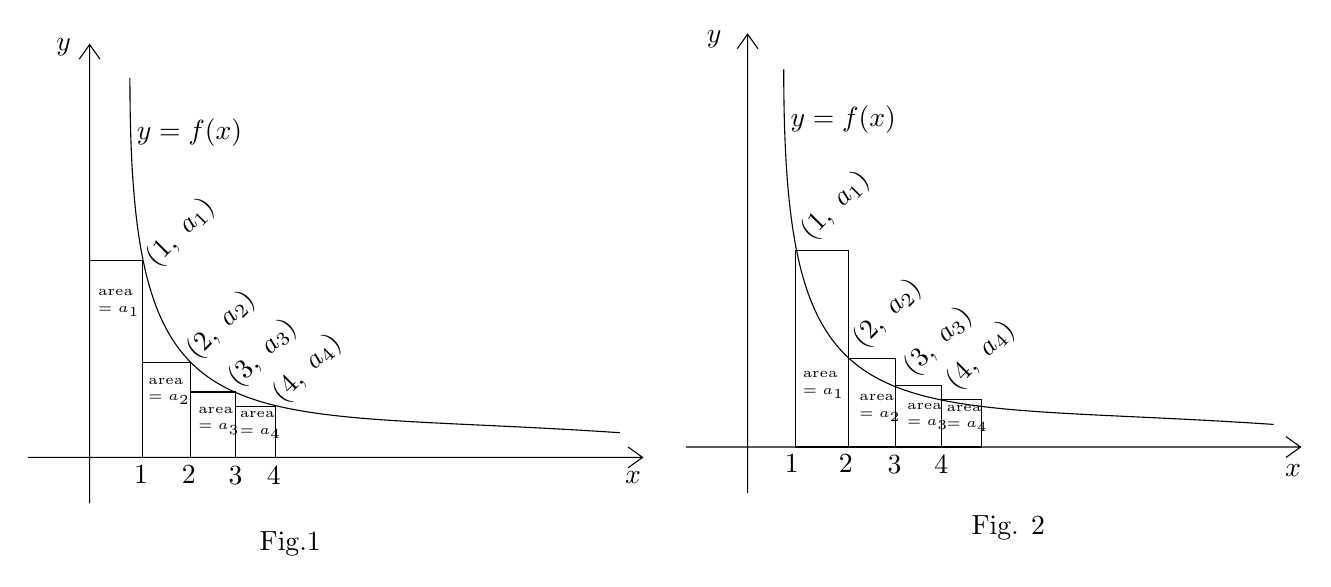
\begin{tikzpicture}[x=0.75pt,y=0.75pt,yscale=-1,xscale=1]
		\draw  (19.74,221.29) -- (315.74,221.29)(49.34,22.39) -- (49.34,243.39) (308.74,216.29) -- (315.74,221.29) -- (308.74,226.29) (44.34,29.39) -- (49.34,22.39) -- (54.34,29.39)  ;
		\draw  (336.74,216.29) -- (632.74,216.29)(366.34,17.39) -- (366.34,238.39) (625.74,211.29) -- (632.74,216.29) -- (625.74,221.29) (361.34,24.39) -- (366.34,17.39) -- (371.34,24.39)  ;
		\draw    (68.74,38.39) .. controls (68.74,221.39) and (112.74,196.39) .. (304.74,209.39) ;
		\draw    (383.74,34.39) .. controls (383.74,217.39) and (427.74,192.39) .. (619.74,205.39) ;
		\draw   (49.34,126.39) -- (74.74,126.39) -- (74.74,221.29) -- (49.34,221.29) -- cycle ;
		\draw   (74.74,175.75) -- (97.74,175.75) -- (97.74,221.29) -- (74.74,221.29) -- cycle ;
		\draw   (97.74,189.75) -- (119.74,189.75) -- (119.74,221.29) -- (97.74,221.29) -- cycle ;
		\draw   (119.74,196.75) -- (138.74,196.75) -- (138.74,221.29) -- (119.74,221.29) -- cycle ;
		\draw   (389.34,121.39) -- (414.74,121.39) -- (414.74,216.29) -- (389.34,216.29) -- cycle ;
		\draw   (414.74,173.75) -- (437.74,173.75) -- (437.74,216.29) -- (414.74,216.29) -- cycle ;
		\draw   (437.74,186.75) -- (459.74,186.75) -- (459.74,216.29) -- (437.74,216.29) -- cycle ;
		\draw   (459.74,193.44) -- (479.05,193.44) -- (479.05,216.29) -- (459.74,216.29) -- cycle ;
		\draw (32,18.01) node [anchor=north west][inner sep=0.75pt]    {$y$};
		\draw (345.5,14.51) node [anchor=north west][inner sep=0.75pt]    {$y$};
		\draw (306,227.01) node [anchor=north west][inner sep=0.75pt]    {$x$};
		\draw (624,223.51) node [anchor=north west][inner sep=0.75pt]    {$x$};
		\draw (70.82,57.01) node [anchor=north west][inner sep=0.75pt]    {$y=f( x)$};
		\draw (385.82,50.51) node [anchor=north west][inner sep=0.75pt]    {$y=f( x)$};
		\draw (69.5,223.88) node [anchor=north west][inner sep=0.75pt]    {$1$};
		\draw (92.5,223.88) node [anchor=north west][inner sep=0.75pt]    {$2$};
		\draw (115,224.38) node [anchor=north west][inner sep=0.75pt]    {$3$};
		\draw (133.5,224.38) node [anchor=north west][inner sep=0.75pt]    {$4$};
		\draw (383,218.88) node [anchor=north west][inner sep=0.75pt]    {$1$};
		\draw (409,218.88) node [anchor=north west][inner sep=0.75pt]    {$2$};
		\draw (432.5,219.38) node [anchor=north west][inner sep=0.75pt]    {$3$};
		\draw (455,219.38) node [anchor=north west][inner sep=0.75pt]    {$4$};
		\draw (72.32,122.76) node [anchor=north west][inner sep=0.75pt]  [rotate=-314.9]  {$( 1,\ a_{1})$};
		\draw (91.83,167.27) node [anchor=north west][inner sep=0.75pt]  [rotate=-314.87]  {$( 2,\ a_{2})$};
		\draw (111.82,180.76) node [anchor=north west][inner sep=0.75pt]  [rotate=-314.9]  {$( 3,\ a_{3})$};
		\draw (133.32,188.26) node [anchor=north west][inner sep=0.75pt]  [rotate=-314.9]  {$( 4,\ a_{4})$};
		\draw (387.82,109.76) node [anchor=north west][inner sep=0.75pt]  [rotate=-314.9]  {$( 1,\ a_{1})$};
		\draw (412.83,161.77) node [anchor=north west][inner sep=0.75pt]  [rotate=-314.87]  {$( 2,\ a_{2})$};
		\draw (437.32,175.26) node [anchor=north west][inner sep=0.75pt]  [rotate=-314.9]  {$( 3,\ a_{3})$};
		\draw (457.82,181.76) node [anchor=north west][inner sep=0.75pt]  [rotate=-314.9]  {$( 4,\ a_{4})$};
		\draw (45.5,136.38) node [anchor=north west][inner sep=0.75pt]  [font=\tiny]  {$ \begin{array}{l}\text{area}\\=a_{1}\end{array}$};
		\draw (69.74,179.15) node [anchor=north west][inner sep=0.75pt]  [font=\tiny]  {$ \begin{array}{l}\text{area}\\=a_{2}\end{array}$};
		\draw (93.74,193.15) node [anchor=north west][inner sep=0.75pt]  [font=\tiny]  {$ \begin{array}{l}\text{area}\\=a_{3}\end{array}$};
		\draw (113.74,195.15) node [anchor=north west][inner sep=0.75pt]  [font=\tiny]  {$ \begin{array}{l}\text{area}\\=a_{4}\end{array}$};
		\draw (385,175.88) node [anchor=north west][inner sep=0.75pt]  [font=\tiny]  {$ \begin{array}{l}\text{area}\\=a_{1}\end{array}$};
		\draw (412.24,187.15) node [anchor=north west][inner sep=0.75pt]  [font=\tiny]  {$ \begin{array}{l}\text{area}\\=a_{2}\end{array}$};
		\draw (435.24,191.15) node [anchor=north west][inner sep=0.75pt]  [font=\tiny]  {$ \begin{array}{l}\text{area}\\=a_{3}\end{array}$};
		\draw (454.24,192.15) node [anchor=north west][inner sep=0.75pt]  [font=\tiny]  {$ \begin{array}{l}\text{area}\\=a_{4}\end{array}$};
		\draw (130,256) node [anchor=north west][inner sep=0.75pt]   [align=left] {Fig.1};
		\draw (473,248) node [anchor=north west][inner sep=0.75pt]   [align=left] {Fig. 2};
	\end{tikzpicture}
	In Fig. 1: $$\sum_{n=2}^\infty a_n\leq\int_1^\infty f(x)\ \dx$$
	Thus, 
	\begin{itemize}
		\item $\displaystyle\sum{a_n}$ diverges $\Longrightarrow\displaystyle\int_1^\infty f(x)\ \dx$ diverges. 
		\item $\displaystyle\int_1^\infty f(x)\ \dx$ converges $\Longrightarrow \displaystyle\sum{a_n}$ converges. 
	\end{itemize}
	In Fig. 2: $$\sum_{n=1}^\infty a_n\geq\int_1^\infty f(x)\ \dx$$
	Thus, 
	\begin{itemize}
		\item $\displaystyle\sum{a_n}$ converges $\Longrightarrow\displaystyle\int_1^\infty f(x)\ \dx$ converges. 
		\item $\displaystyle\int_1^\infty f(x)\ \dx$ diverges $\Longrightarrow \displaystyle\sum{a_n}$ diverges. 
	\end{itemize}
\end{prf}
\begin{eg}{Example 1}
	Show that the harmonic series, $\displaystyle\sum_{n=1}^\infty\frac{1}{n}$, diverges. \\
	\noindent\rule[0.25\baselineskip]{\textwidth}{1pt}
	Let $\displaystyle f(x)=\frac{1}{x}$
	\begin{enumerate}
		\item Show $f(x)$ satisfies conditions for integral test: 
		\begin{itemize}
			\item $\displaystyle f(x)=\frac{1}{x}\geq0\quad\forall x\geq 1$, obvious.
			\item $\displaystyle f'(x)=-\frac{1}{x^2}$ is defined $\forall x\geq1$\\
			$\Rightarrow f(x)$ is differentiable $\forall x\geq1$\\
			$\Rightarrow f(x)$ is continuous $\forall x\geq1$
			\item $\displaystyle f'(x)=-\frac{1}{x^2}<0\quad\forall x\geq1$\\
			$\Rightarrow f(x)$ is decreasing $\forall x\geq1$
		\end{itemize}
		\item Use the integral test to show $\displaystyle\sum_{n=1}^\infty\frac{1}{n}$ diverges: 
		$$\begin{aligned}
			\int_1^\infty f(x)\ \dx &=\int_1^\infty\frac{1}{x}\ \dx\\
			&=\lim_{t\to\infty}\int_1^t\frac{1}{x}\ \dx\\
			&=\lim_{t\to\infty}\bigg[\ln{x}\bigg]_1^t\\
			&=\lim_{t\to\infty}(\ln{t}-\ln1)\\
			&=\lim_{t\to\infty}\ln{t}=\infty
		\end{aligned}$$
		$$\therefore \int_1^\infty\frac{1}{x}\ \dx \text{diverges}$$
		By the integral test, $\displaystyle\sum_{n=1}^\infty\frac{1}{n}$ also diverges.
	\end{enumerate}
\end{eg}
\begin{eg}{Example 2}
	Consider the series $\displaystyle\sum_{n=1}^\infty\frac{1}{n^p}$, where $p>0$ is a constant. \\
	\noindent\rule[0.25\baselineskip]{\textwidth}{1pt}
	Note: $p=1\ \Rightarrow$ harmonic series $\Rightarrow$ diverges. So consider $p\neq1$: \\
	Let $\displaystyle f(x)=\frac{1}{x^p}=x^{-p}$
	\begin{enumerate}
		\item Show that $f(x)$ satisfies conditions of integral test: 
		\begin{itemize}
			\item $\displaystyle f(x)=\frac{1}{x^p}>0\quad\forall x\geq1\text{ and }p>0$
			\item $\displaystyle f'(x)=\frac{-p}{x^{p+1}}$ is defined $\forall x\geq1$ and $p>0$.\\
			$\therefore f(x)$ us continuous $\forall x\geq1$ and $p>0$.
			\item $f'(x)=\frac{-p}{x^{p+1}}<0 \forall x\geq1$ and $p>0$.\\
			$\Rightarrow f(x)$ is decreasing $\forall x\geq1$.
		\end{itemize}
		\item Use the integral test to determine convergence or divergence of $\displaystyle\sum_{n=1}^\infty\frac{1}{n},\ p\neq1$: \\
		Recall from section \ref{improper}: 
		$$\int_1^\infty\frac{1}{x^p}\ \dx\text{ is }\begin{cases}\text{convergent if }p>1\\\text{divergent if }p\leq1\end{cases}$$
		By the integral test: 
		$$\sum_{n=1}^\infty\frac{1}{n^p}\ \dx\text{ is }\begin{cases}\text{convergent if }p>1\\\text{divergent if }p\leq1\end{cases}$$
	\end{enumerate}
\end{eg}
\begin{rmk}{$p$-Series}
	$$\sum_{n=1}^\infty\frac{1}{n^p}\text{ converges if} p>1\text{, and diverges if }p\leq1.$$
\end{rmk}
\begin{eg}{Remainder Estimation}
	How can we estimate $\displaystyle S=\sum_{n=1}^\infty{a_n}$\\
	\noindent\rule[0.25\baselineskip]{\textwidth}{1pt}
	\begin{itemize}
		\item Choose fixed (large) value to replace $\infty$, and complete $$S_n=\sum_{k=1}^n{a_k}\approx S.$$
		\item Question: How good is this estimation? \\
		$$\begin{aligned}
			R_n&=S-S_n\quad\text{(residual/reminder)}\\
			&=(a_1+a_2+a_3+\cdots+a_n+a_{n+1}+a_{n+2}+\cdots)\\
			&\quad-(a_1+a_2+a_3+\cdots+a_n)\\
			&=a_{n+1}+a_{n+2}+a_{n+3}\cdots
		\end{aligned}$$ 
		Our new question is: \underline{How big is $R_n$?}\\
		Let $f(x)$ be a function with $f(x)=a_n$, we can draw the following figures.
		\tikzset{every picture/.style={line width=0.75pt}} 
		\begin{tikzpicture}[x=0.75pt,y=0.75pt,yscale=-1,xscale=1]
		\draw  (19.74,180.95) -- (243.49,180.95)(42.11,20.41) -- (42.11,198.79) (236.49,175.95) -- (243.49,180.95) -- (236.49,185.95) (37.11,27.41) -- (42.11,20.41) -- (47.11,27.41)  ;
		\draw  (259.37,176.92) -- (483.12,176.92)(281.74,16.37) -- (281.74,194.76) (476.12,171.92) -- (483.12,176.92) -- (476.12,181.92) (276.74,23.37) -- (281.74,16.37) -- (286.74,23.37)  ;
		\draw    (56.78,33.32) .. controls (56.78,181.03) and (90.04,160.86) .. (235.18,171.35) ;
		\draw    (294.9,30.09) .. controls (294.9,177.81) and (328.16,157.63) .. (473.3,168.12) ;
		\draw   (61.31,144.2) -- (78.7,144.2) -- (78.7,180.95) -- (61.31,180.95) -- cycle ;
		\draw   (78.7,155.5) -- (95.33,155.5) -- (95.33,180.95) -- (78.7,180.95) -- cycle ;
		\draw   (95.33,161.15) -- (109.69,161.15) -- (109.69,180.95) -- (95.33,180.95) -- cycle ;
		\draw   (318.33,142.58) -- (335.72,142.58) -- (335.72,176.92) -- (318.33,176.92) -- cycle ;
		\draw   (335.72,153.08) -- (352.35,153.08) -- (352.35,176.92) -- (335.72,176.92) -- cycle ;
		\draw   (352.35,158.48) -- (366.95,158.48) -- (366.95,176.92) -- (352.35,176.92) -- cycle ;
		\draw (27.54,15.41) node [anchor=north west][inner sep=0.75pt]    {$y$};
		\draw (264.53,12.58) node [anchor=north west][inner sep=0.75pt]    {$y$};
		\draw (234.67,184.11) node [anchor=north west][inner sep=0.75pt]    {$x$};
		\draw (475.06,181.28) node [anchor=north west][inner sep=0.75pt]    {$x$};
		\draw (55.89,183.49) node [anchor=north west][inner sep=0.75pt]  [font=\normalsize]  {$n$};
		\draw (98.82,207.43) node [anchor=north west][inner sep=0.75pt]   [align=left] {Fig.1};
		\draw (357.61,200.97) node [anchor=north west][inner sep=0.75pt]   [align=left] {Fig. 2};
		\draw (299.42,180.39) node [anchor=north west][inner sep=0.75pt]  [font=\normalsize]  {$n+1$};
	\end{tikzpicture}	
	
	From Fig. 1, $$\begin{aligned}\text{Area}: a_{n+1}+a_{n+2}+a_{n+3}+\cdots &=R_n\\ \int_n^\infty f(x)\ \dx &\geq R_n \end{aligned}$$
 	From Fig. 2, $$\begin{aligned}\text{Area}: a_{n+1}+a_{n+2}+a_{n+3}+\cdots &=R_n\\ \int_{n+1}^\infty f(x)\ \dx &\leq R_n \end{aligned}$$
 	That is, 
 	$$\int_{n+1}^\infty f(x)\ \dx\leq R_n\leq\int_n^\infty f(x)\ \dx$$
	\end{itemize}
\end{eg}
\begin{thm}{Remainder Estimate for Partial Sums}
	If $\displaystyle S=\sum_{k=1}^\infty{a_k}$ and $\displaystyle S_n=\sum_{k=1}^n{a_k}=n$th partial sums, and $$R_n=S-S_n,$$ then $$\int_{n+1}^\infty f(x)\ \dx\leq R_n\leq\int_n^\infty f(x)\ \dx$$	 where $f(x)$ is a function with $f(n)=a_n.$
\end{thm}
\begin{eg}{Example 3}
	Consider the series $\displaystyle\sum_{k=2}^\infty\frac{1}{k(\ln{k})^2}$.\\
	\noindent\rule[0.25\baselineskip]{\textwidth}{1pt}
	\begin{enumerate}
		\item Show that this series converges by the integral test.
		\item How many terms do we need in $$S_n=\sum_{k=2}^n\frac{1}{k(\ln{k})^2}$$ so that $S_n$ is accurate estimation to $0.01$? \\
		That is, we want to choose $n$ large enough so that $$R_n<0.01.$$	
		We know $$R_n\leq\int_n^\infty\frac{1}{x(\ln{x})^2}\ \dx$$
		$$\begin{aligned}
			\int_n^\infty\frac{1}{x(\ln{x})^2}\ \dx&=\lim_{t\to\infty}\int_n^t\frac{1}{x(\ln{x})^2}\ \dx\\
			&=\lim_{t\to\infty}\bigg[-\frac{1}{\ln{x}}\bigg]_n^t\\
			&=\lim_{t\to\infty}\left(-\frac{1}{\ln{t}}+\frac{1}{\ln{n}}\right)\\
			&=\frac{1}{\ln{n}}
		\end{aligned}$$
		$\therefore$ we need $$\begin{aligned}
			\frac{1}{\ln{n}}&<0.01\\
			\ln{n}&>100\\
			n&>e^{100}\quad(\approx2.7\times10^{43})
		\end{aligned}$$
		This is a really large number!
	\end{enumerate}
\end{eg}

\subsection{Comparison Tests}
\begin{thm}{Basic Comparison Test}
	Suppose $\displaystyle\sum{a_n}$ and $\displaystyle\sum{b_n}$ are positive terms. Then
	\begin{enumerate}
		\item If $\displaystyle\sum{b_n}$ converges and $a_n\leq b_n\ \forall n$,\\
		then $\displaystyle\sum{a_n}$ also converges.
		\item 	If $\displaystyle\sum{b_n}$ diverges and $a_n\geq b_n\ \forall n$,\\
		then $\displaystyle\sum{a_n}$ also diverges.
	\end{enumerate}
\end{thm}
\begin{eg}{Example 1}
	Consider the series $\displaystyle\sum_{n=2}^\infty\frac{1}{\sqrt{n}-1}$	\\
	\noindent\rule[0.25\baselineskip]{\textwidth}{1pt}
	\begin{enumerate}
		\item Compare $\displaystyle\frac{1}{\sqrt{n}-1}$ and $\displaystyle\frac{1}{\sqrt{n}}$: 
		$$\frac{1}{\sqrt{n}-1}>\frac{1}{\sqrt{n}}\ \forall n\geq 2$$
		\item $\displaystyle\sum_{n=2}^\infty\frac{1}{\sqrt{n}}=sum_{n=2}^\infty\frac{1}{n^{1/2}}$ is a divergent $p$-series with $\displaystyle p=\frac{1}{2}$
	\end{enumerate}
	By the comparison test, 
	$$\sum_{n=2}^\infty\frac{1}{\sqrt{n}-1}\text{ also diverges.}$$
\end{eg}
\begin{eg}{Example 2}
	Consider the series $\displaystyle\sum_{n=1}^\infty\frac{n-1}{n^3+1}$\\
	\noindent\rule[0.25\baselineskip]{\textwidth}{1pt}
	\begin{itemize}
		\item $\displaystyle\frac{n-1}{n^3+1}<\frac{n}{n^3+1}<\frac{n}{n^3}=\frac{1}{n^2}$
		\item $\displaystyle\sum_{n=1}^\infty\frac{1}{n^2}$ is a convergent $p$-series with $p=2>1$.
	\end{itemize}
	$\therefore$ By comparison test,
	$$\sum_{n=1}^\infty\frac{n-1}{n^3+1}\text{ also converges.}$$
\end{eg}
\begin{eg}{Example 3}
	Consider the series $\displaystyle\sum_{n=1}^\infty\frac{6^n}{5^n-1}$\\	
	\noindent\rule[0.25\baselineskip]{\textwidth}{1pt}
	\begin{itemize}
		\item $\displaystyle\frac{6^n}{5^n-1}>\frac{6^n}{5^n}=\left(\frac{6}{5}\right)^n$
		\item $\displaystyle\sum_{n=1}^\infty\left(\frac{6}{5}\right)^n$ is a divergent geometric sequence with $$|r|=\frac{6}{5}>1$$
	\end{itemize}
	$\therefore$ By comparison test,
	$$\sum_{n=1}^\infty\frac{6^n}{5^n-1}\text{ also diverges.}$$
\end{eg}
\begin{eg}{Example 4}
	Consider the series $\displaystyle\sum_{k=1}^\infty\frac{(2k-1)(k^2-1)}{(k+1)(k^2+4)^2}$\\
	\noindent\rule[0.25\baselineskip]{\textwidth}{1pt}
	\begin{itemize}
		\item $\displaystyle\frac{(2k-1)(k^2-1)}{(k+1)(k^2+4)^2}=\frac{(2k-1)(k-1)(k+1)}{(k+1)(k^2+4)^2}=\frac{(2k-1)(k-1)}{(k^2+4)^2}<\frac{(2k)(k)}{(k^2+4)^2}<\frac{2k^2}{(k^2)^2}=\frac{2}{k^2}$	
		\item $\displaystyle\sum_{k=1}^\infty\frac{2}{k^2}$ is a convergent $p$-series with $p=2>1$.
	\end{itemize}
	$\therefore$ By comparison test, 
	$$\sum_{k=1}^\infty\frac{(2k-1)(k^2-1)}{(k+1)(k^2+4)^2}\text{ also converges.}$$
\end{eg}
\begin{eg}{Example 5}
	Consider the series $\displaystyle\sum_{n=1}^\infty\frac{1}{n^n}$\\
	\noindent\rule[0.25\baselineskip]{\textwidth}{1pt}
	\begin{itemize}
		\item $\displaystyle\frac{1}{n^n}=\frac{1}{n\cdots n}\leq\frac{1}{n^2}$
		\item $\displaystyle\sum_{n=1}^\infty\frac{1}{n^2}$ is a convergent $p$-series with $p=2>1$
	\end{itemize}
	$therefore$ By comparison test,
	$$\sum_{n=1}^\infty\frac{1}{n^n}\text{ also converges.}$$
\end{eg}
\begin{thm}{Limit Comparison Test}
	Suppose $\displaystyle\sum{a_n}$ and $\displaystyle\sum{b_n}$ are positive term series. If $$\lim_{n\to\infty}\frac{a_n}{b_n}=C,\ \text{ where }C>0\text{ is finite,}$$ then either both series converge or both series diverge.	
\end{thm}
\begin{eg}{Example 6}
	Consider the series $\displaystyle\sum_{n=1}^\infty\frac{2}{\sqrt{n}+2}$\\
	\noindent\rule[0.25\baselineskip]{\textwidth}{1pt}
	\begin{itemize}
		\item Let $\displaystyle a_n=\frac{2}{\sqrt{n}+2}$ and $\displaystyle b_n=\frac{1}{\sqrt{n}}$
		\item $\displaystyle\lim_{n\to\infty}\frac{a_n}{b_n}=\lim_{n\to\infty}\frac{2}{\sqrt{n}+2}\cdot\frac{\sqrt{n}}{1}=\lim_{n\to\infty}\frac{2\sqrt{n}}{\sqrt{n}+2}=\lim_{n\to\infty}\frac{2}{1+\frac{2}{\sqrt{n}}}=2>0$
		\item $\displaystyle \sum_{n=1}^\infty\frac{1}{\sqrt{n}}$ is a divergent $p$-series, with $\displaystyle p=\frac{1}{2}<1$
	\end{itemize}
	$\therefore$ By limit comparison test,
	$$\sum_{n=1}^\infty\frac{2}{\sqrt{n}+2}\text{ also diverges.}$$
\end{eg}
\begin{eg}{Example 7}
	Consider the series $\displaystyle\sum_{n=1}^\infty\frac{n^2+n+1}{n^4+n^2}$\\
	\noindent\rule[0.25\baselineskip]{\textwidth}{1pt}
	\begin{itemize}
		\item Let $\displaystyle a_n=\frac{n^2+n+1}{n^4+n^2}$ and $\displaystyle b_n=\frac{1}{n^2}$
		\item $$\begin{aligned}
					\lim_{n\to\infty}\frac{a_n}{b_n}=\lim_{n\to\infty}\frac{n^2+n+1}{n^4+n^2}\cdot n^2&=\lim_{n\to\infty}\frac{(n^2+n+1)n^2}{n^2(n^2+1)}\\
					&=\lim_{n\to\infty}\frac{n^2+n+1}{n^2+1}\\
					&=\lim_{n\to\infty}\frac{1+\frac{1}{n}+\frac{1}{n^2}}{1+\frac{1}{n^2}}=1>0
				\end{aligned}$$
		\item $\displaystyle \sum_{n=1}^\infty\frac{1}{n^2}$ is a convergent $p$-series, with $p=2>1$.
	\end{itemize}
	$\therefore$ By the limit comparison test, 
	$$\sum_{n=1}^\infty\frac{n^2+n+1}{n^4+n^2}\text{ also converges.}$$
\end{eg}
\begin{eg}{Example 8}
	Consider the series $\displaystyle\sum_{n=1}^\infty\frac{1}{n^{1+1/n}}$\\
	\noindent\rule[0.25\baselineskip]{\textwidth}{1pt}
	\begin{itemize}
		\item Let $\displaystyle a_n=\frac{1}{n^{1+1/n}}=\frac{1}{n\cdot n^{1/n}}$ and $\displaystyle b_n=\frac{1}{n}$
		\item $\displaystyle \lim_{n\to\infty}\frac{1_n}{b_n}=\lim_{n\to\infty}\frac{1}{n\cdot n^{1/n}}\cdot n=\lim_{n\to\infty}\frac{1}{n^{1/n}}$ \\
			We need to find $\displaystyle\lim_{n\to\infty}n^{\frac{1}{n}}:$\\
			Let $f(x)=x^{\frac{1}{x}}$, look at $\displaystyle\lim_{x\to\infty}x^{\frac{1}{x}}$ is in indeterminant form $\infty^0$.
			$$\lim_{x\to\infty}e^{\ln{x^{1/x}}}=\lim_{x\to\infty}e^{\frac{1}{x}\ln{x}}=e^{\lim_{x\to\infty}\frac{\ln{x}}{x}}$$
			Find $\displaystyle\lim_{x\to\infty}\frac{\ln{x}}{x}$ in indeterminant form of $\displaystyle\frac{\infty}{\infty}$ by applying L'Hopital's rule: 
			$$\lim_{x\to\infty}\frac{\ln{x}}{x}=\lim_{x\to\infty}\frac{\frac{1}{x}}{1}=\lim_{x\to\infty}\frac{1}{x}=0$$
			$$\therefore \lim_{x\to\infty}x^{\frac{1}{x}}=\lim_{x\to\infty} e^{\ln{x^{1/x}}}=e^{\lim_{x\to\infty}\frac{\ln{x}}{x}}=e^0=1$$
			$$\therefore\lim_{n\to\infty}n^{\frac{1}{n}}=\lim_{x\to\infty}x^{\frac{1}{x}}=1\qquad\text{(By the function method)}$$
			$$\therefore\lim_{n\to\infty}\frac{a_n}{b_n}=\lim_{n\to\infty}\frac{1}{n^{1/n}}=\frac{1}{1}=1>0$$
		\item $\displaystyle\sum_{n=1}^\infty\frac{1}{n}$ is the harmonic series, divergent.
	\end{itemize}
	$\therefore$ By the limit comparison test, 
	$$\sum_{n=1}^\infty\frac{1}{n^{1+1/n}}\text{ also diverges.}$$
\end{eg}

\subsection{Alternating Series Test}\label{Alternating}
\begin{rmk}{Review of Important Series}
	$$\begin{aligned}
		\textbf{Geometric:}\quad &\sum^\infty_{n=1}{ar^{n-1}}=a\left(1+r+r^2+\cdots\right),\quad a\neq0\\
		&\text{if }|r|<1\text{ the series converges, and }\sum^\infty_{n=1}a r^{n-1}=\frac{a}{1-r}\\
		p-\textbf{Series:}\quad &\sum^\infty_{n=1}\frac{1}{n^p}\begin{cases}\text{converges if} p>1\\\text{diverges if }p\leq1\end{cases}\text{(prove with integral test)}\\
		\textbf{Harmonic:}\quad &\sum^\infty_{n=1}\frac{1}{n}\text{ diverges (prove with integral test)}\\
		\textbf{Alternating Harmonic:}\quad &\sum_{n=1}^\infty(-1)^{n-1}\frac{1}{n}\text{ converges to }\ln{2}
	\end{aligned}$$
\end{rmk}
However, the alternating harmonic series was not proven to be convergent in previous sections, which will be done in this section. 
\begin{prf}{Convergence of Alternating Harmonic Series}
	Consider the partial sum: 
	$$\begin{aligned}
		S_{2n}=\sum_{k=1}^{2n}(-1)^{k-1}\frac{1}{k}&=1-\frac{1}{2}+\frac{1}{3}-\frac{1}{4}+\cdots+\frac{1}{2n-1}-\frac{1}{2n}\\
		&=\sum_{k=1}^{n}\left(\frac{1}{2k-1}-\frac{1}{k}\right)\\
		&=\sum_{k=1}^{n}\left(\frac{1}{2k-1}{\color{red}{+\frac{1}{2k}-\frac{1}{2k}}}-\frac{1}{2k} \right)\\
		&=\sum_{k=1}^{n}\left(\frac{1}{2k-1}+\frac{1}{2k}\right)-2\sum_{k=1}^{n}\left(\frac{1}{2k}\right)\\
		&=\left(1+\frac{1}{2}+\cdots+\frac{1}{n}+\frac{1}{n+1}+\cdots+\frac{1}{2n-1}+\frac{1}{2n}\right)-\underbrace{2\left(\frac{1}{2}+\frac{1}{4}+\cdots+\frac{1}{2n}\right)}_{\color{red}{1+\frac{1}{2}+\frac{1}{3}+\cdots+\frac{1}{n}}}\\
		&=\frac{1}{n+1}+\frac{1}{n+2}+\cdots+\frac{1}{2n-1}+\frac{1}{2n}\\
		&=\sum_{k=n+1}^{2n}\frac{1}{k}\quad\Longrightarrow\text{ We need to find }\lim_{n\to\infty}S_{2n}=\lim_{k\to\infty}\sum_{k=n+1}^{2n}\frac{1}{k}.
	\end{aligned}$$	
	\tikzset{every picture/.style={line width=0.75pt}}
		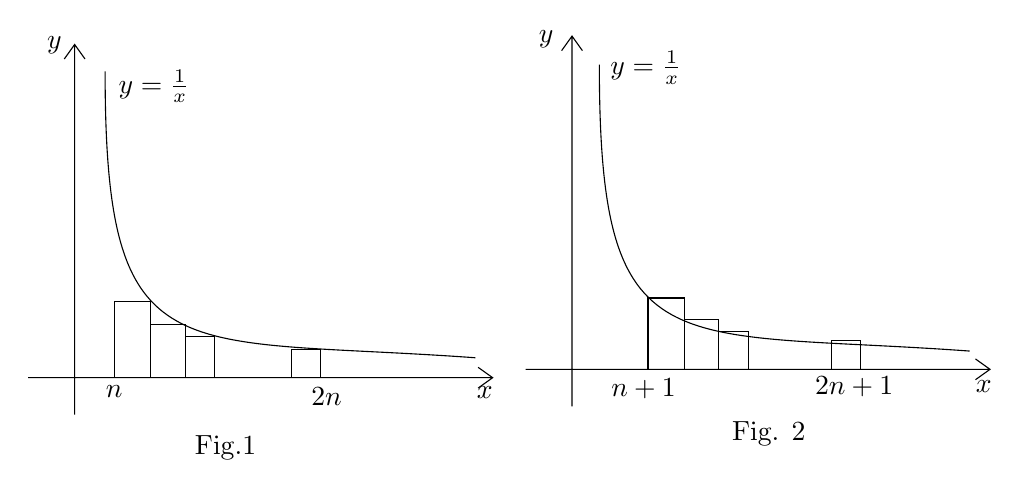
\begin{tikzpicture}[x=0.75pt,y=0.75pt,yscale=-1,xscale=1]
		\draw  (19.74,180.95) -- (243.49,180.95)(42.11,20.41) -- (42.11,198.79) (236.49,175.95) -- (243.49,180.95) -- (236.49,185.95) (37.11,27.41) -- (42.11,20.41) -- (47.11,27.41)  ;
		\draw  (259.37,176.92) -- (483.12,176.92)(281.74,16.37) -- (281.74,194.76) (476.12,171.92) -- (483.12,176.92) -- (476.12,181.92) (276.74,23.37) -- (281.74,16.37) -- (286.74,23.37)  ;
		\draw    (56.78,33.32) .. controls (56.78,181.03) and (90.04,160.86) .. (235.18,171.35) ;
		\draw    (294.9,30.09) .. controls (294.9,177.81) and (328.16,157.63) .. (473.3,168.12) ;
		\draw   (61.31,144.2) -- (78.7,144.2) -- (78.7,180.95) -- (61.31,180.95) -- cycle ;
		\draw   (78.7,155.5) -- (95.33,155.5) -- (95.33,180.95) -- (78.7,180.95) -- cycle ;
		\draw   (95.33,161.15) -- (109.69,161.15) -- (109.69,180.95) -- (95.33,180.95) -- cycle ;
		\draw   (318.33,142.58) -- (335.72,142.58) -- (335.72,176.92) -- (318.33,176.92) -- cycle ;
		\draw   (335.72,153.08) -- (352.35,153.08) -- (352.35,176.92) -- (335.72,176.92) -- cycle ;
		\draw   (352.35,158.48) -- (366.95,158.48) -- (366.95,176.92) -- (352.35,176.92) -- cycle ;
		\draw   (146.56,167.22) -- (160.69,167.22) -- (160.69,180.95) -- (146.56,180.95) -- cycle ;
		\draw   (406.56,163.22) -- (420.69,163.22) -- (420.69,176.95) -- (406.56,176.95) -- cycle ;
		\draw (27.54,15.41) node [anchor=north west][inner sep=0.75pt]    {$y$};
		\draw (264.53,12.58) node [anchor=north west][inner sep=0.75pt]    {$y$};
		\draw (234.67,184.11) node [anchor=north west][inner sep=0.75pt]    {$x$};
		\draw (475.06,181.28) node [anchor=north west][inner sep=0.75pt]    {$x$};
		\draw (55.89,183.49) node [anchor=north west][inner sep=0.75pt]  [font=\normalsize]  {$n$};
		\draw (98.82,207.43) node [anchor=north west][inner sep=0.75pt]   [align=left] {Fig.1};
		\draw (357.61,200.97) node [anchor=north west][inner sep=0.75pt]   [align=left] {Fig. 2};
		\draw (299.42,180.39) node [anchor=north west][inner sep=0.75pt]  [font=\normalsize]  {$n+1$};
		\draw (62,31.4) node [anchor=north west][inner sep=0.75pt]    {$y=\frac{1}{x}$};
		\draw (299,22.4) node [anchor=north west][inner sep=0.75pt]    {$y=\frac{1}{x}$};
		\draw (154.89,184.49) node [anchor=north west][inner sep=0.75pt]  [font=\normalsize]  {$2n$};
		\draw (397.56,179.35) node [anchor=north west][inner sep=0.75pt]  [font=\normalsize]  {$2n+1$};
	\end{tikzpicture}
	\\From Fig.1, we know 
	$$\begin{aligned}
		\frac{1}{n+1}+\cdots+\frac{1}{2n}&\leq\int_n^{2n}\frac{1}{x}\ \dx\\
		S_{2n}&\leq\int_n^{2n}\frac{1}{x}\ \dx
	\end{aligned}$$
	From Fig.2, we know 
	$$\begin{aligned}
		\frac{1}{n+1}+\cdots+\frac{1}{2n}&\geq\int_{n+1}^{2n+1}\frac{1}{x}\ \dx\\
		S_{2n}&\geq\int_{n+1}^{2n+1}\frac{1}{x}\ \dx
	\end{aligned}$$
	$${\color{red}{\therefore \int_{n+1}^{2n+1}\frac{1}{x}\ \dx\leq S_{2n}\leq\int_n^{2n}\frac{1}{x}\ \dx}}$$
	Do the integrals: 
	\begin{itemize}
		\item $$\int_{n+1}^{2n+1}\frac{1}{x}\ \dx=\Big[\ln{x}\Big]^{2n+1}_{n+1}=\ln{(2n+1)}-\ln{(n+1)}=\ln\left(\frac{2n+1}{n+1}\right)$$
		\item $$\int_n^{2n}\frac{1}{x}\ \dx=\Big[\ln{x}\Big]^{2n}_{n}=\ln(2n)-\ln(n)=\ln\left(\frac{2n}{n}\right)=\ln{2}$$
	\end{itemize}
	That is, $$\ln\left(\frac{2n+1}{n+1}\right)\leq S_{2n}\leq\ln{2}$$
	Notice, $$\begin{aligned}
		\lim_{n\to\infty}\ln\left(\frac{2n+1}{n+1}\right)&=\lim_{n\to\infty}\ln\left(\frac{2+1/n}{1+1/n}\right)\\
		&=\ln{2}\\
		\lim_{n\to\infty}\ln{2}&=\ln{2}
	\end{aligned}$$
	$$\therefore \text{ When }n\to\infty:\quad\ln{2}\leq S_{2n}\leq\ln{2}$$
	By the squeeze theorem, 
	$$\lim_{n\to\infty}S_{2n}=\ln{2}$$
	i.e., 
	$$\sum_{n=1}^\infty(-1)^{n-1}\frac{1}{n}=\ln{2}$$
\end{prf}
However, we still need a test for other alternating series. 
\begin{thm}{Alternating Series Test}
	If the alternating series: $$\sum_{n=1}^\infty(-1)^{n-1}b_n$$ satisfies $b_n\geq b_{n+1}$ and $\displaystyle\lim_{n\to\infty}b_n=0$, then the series converges. 
\end{thm}
\begin{prf}{Proof}
	To see why the series converges: 
	$$\begin{aligned}
		S_{2n}&=(b_1-b_2)+\cdots+(b_{2n-1}-b_{2n})\quad\text{[Adding non-negative numbers]}\\
		&=b_1-(b_2-b_3)-\cdots-(b_{2n-2}-b_{2n-1})-b_{2n}\quad\text{[Subtracting non-negative numbers]}
	\end{aligned}$$	
	$$b_1\geq b_2\ \Rightarrow\ b_1-b_2\geq0, \cdots, b_{2n-1}\geq b_{2n}\ \Rightarrow\ b_{2n-1}-b_{2n}\geq0$$
	This means: 
	\begin{itemize}
		\item Even numbered partial sums are increasing non-negative numbers
		\item But they are bounded above by $b_1$
		\item $\displaystyle\lim_{n\to\infty}S_{2n}$ converges to, say, $S$.	
	\end{itemize}
	Now, let's consider odd numbered partial sums: 
	$$\begin{aligned}
		S_{2n+1}&=b_1-b_2+b_3-b_4+\cdots+b_{2n-1}-b_{2n}+b_{2n+1}\\
		&=S_{2n}+b_{2n+1}
	\end{aligned}$$
	$$\begin{aligned}
		\lim_{n\to\infty}S_{2n+1}&=\lim_{n\to\infty}\left(S_{2n}+b_{2n+1}\right)\\
		&=\lim_{n\to\infty}S_{2n}+\lim_{n\to\infty}b_{2n+1}\\
		&=S+0
	\end{aligned}$$
	$$\therefore \lim_{n\to\infty}S_{2n+1}=S=\lim_{n\to\infty}S_{2n}$$
\end{prf}
\begin{eg}{Example 1}
	Consider the series $\displaystyle\sum_{n=1}^\infty n^{-1/2}$\\
	\noindent\rule[0.25\baselineskip]{\textwidth}{1pt}
	This is a divergent $p$-series, with $\displaystyle p=\frac{1}{2}<1$
\end{eg}
\begin{eg}{Example 2}
	Consider the series $\displaystyle\sum_{n=1}^\infty (-1)^nn^{-1/2}$\\
	\noindent\rule[0.25\baselineskip]{\textwidth}{1pt}
	Notice: 
	\begin{itemize}
		\item $\displaystyle b_n=\frac{1}{n^{1/2}},\ b_{n+1}=\frac{1}{(n+1)^{1/2}}$
		\item $\displaystyle\lim_{n\to\infty}b_n=\lim_{n\to\infty}\frac{1}{\sqrt{n}}=0$
	\end{itemize}
	$\therefore$ By the alternating series test, 
	$$\sum^\infty_{n=1}(-1)^nn^{-1/2}\text{ converges.}$$
\end{eg}
\begin{eg}{Example 3}
	Consider the series $\displaystyle\sum_{n=1}^\infty (-1)^{n+1}\frac{n^2}{n^3+4}$\\
	\noindent\rule[0.25\baselineskip]{\textwidth}{1pt}
	This is an alternating series, with $\displaystyle b_n=\frac{n^2}{n^3+4}$
	\begin{itemize}
		\item Let $\displaystyle f(x)=\frac{x^2}{x^3+4},\ \text{with }f(n)=b_n$
		$$\begin{aligned}
			f'(x)=\frac{2x(x^3+4)-x^2(3x^2)}{(x^3+4)^2}&=\frac{2x^4+8x-3x^4}{(x^3+4)^2}\\
			&=\frac{8x-x^4}{(x^3+4)^2}\\
			&=\frac{x(x^3-8)}{(x^3+4)^2}=\frac{x(2-x)(x^2+2x+1)}{(x^3+4)^2}
		\end{aligned}$$
		$$\begin{aligned}
			\therefore\ &f'(x)<0\ \forall x>2\\
			\therefore\ &f'(x)\text{ is decreasing }\forall x>2\\
			\therefore\ &b_n=\frac{n^2}{n^3+4}\text{ is decreasing }\forall n>2\ \text{[by the function method]}
		\end{aligned}$$
		\item $\displaystyle\lim_{n\to\infty}\frac{n^2}{n^3+4}=\lim_{n\to\infty}\frac{1/n}{1+4/n^2}=0$
	\end{itemize}
	$\therefore$ By the alternating series test, 
	$$\sum_{n=1}^\infty (-1)^n\frac{n^2}{n^3+4}\text{ converges.}$$
\end{eg}
\begin{eg}{Example 4}
	Consider the series $\displaystyle\sum_{n=1}^\infty (-1)^{n-1}\frac{n}{2n+1}$\\
	\noindent\rule[0.25\baselineskip]{\textwidth}{1pt}
	In this case, the series diverges because 
	$$\lim_{n\to\infty}\frac{n}{2n+1}=\lim_{n\to\infty}\frac{1}{2+1/n}=\frac{1}{2}\neq0$$
	$$\text{[the }n\text{-th term test]}$$
\end{eg}
\begin{eg}{Example 5}
	Consider the series $\displaystyle\sum_{n=1}^\infty (-1)^{n-1}\ln\left(\frac{n+1}{n}\right)$\\
	\noindent\rule[0.25\baselineskip]{\textwidth}{1pt}
	Here, $\displaystyle b_n=\ln\left(\frac{n+1}{n}\right)$
	\begin{itemize}
		\item $\displaystyle\lim_{n\to\infty}\ln\left(\frac{n+1}{n}\right)=\lim_{n\to\infty}\ln\left(\frac{1+1/n}{1}\right)=\ln(1)=0$
		\item Show that $b_n$ is decreasing: \\
		Let $\displaystyle f(x)=\ln\left(\frac{x+1}{x}\right)$ with $f(n)=b_n,\ x>0.$
		$$f(x)=\ln\left(\frac{x+1}{x}\right)=\ln(x+1)-\ln(x)$$
		$$\therefore\ f'(x)=\frac{1}{x+1}-\frac{1}{x}=\frac{-1}{x(x+1)}<0\ \forall x>0$$
		$$f(x)\text{ is decreasing }\forall x>0$$
		$$\therefore\ b_n=\ln\left(\frac{n+1}{n}\right)\text{ is decreasing by the function method}$$
	\end{itemize}
	$\therefore$ By the alternating series test,
	$$\sum_{n=1}^\infty(-1)^{n-1}\ln\left(\frac{n+1}{n}\right)\text{ converges.}$$
\end{eg}

\subsection{Absolute Convergence and the Ratio and Root Tests}
\begin{df}{Absolute Convergence}
	If $\displaystyle \sum|a_n|$ converges, then we say that $\displaystyle \sum{a_n}$ is \underline{absolutely convergent}.	
\end{df}
\begin{thm}{Absolute Convergence Test}
	If $\displaystyle \sum{a_n}$ is absolutely convergent, then it is convergent. 	
\end{thm}
\begin{eg}{Example 1}
	Consider the series $\displaystyle\sum_{n=1}^\infty(-1)^{n-1}\frac{1}{n^2}$\\
	\noindent\rule[0.25\baselineskip]{\textwidth}{1pt}	
	Here $\displaystyle a_n=(-1)^{n-1}\frac{1}{n^2}$ and $\displaystyle|a_n|=\frac{1}{n^2}$\\
	Notice: \\$\displaystyle\sum^\infty_{n=1}|a_n|=\sum^\infty_{n=1}\frac{1}{n^2}$ is a convergent $p$-series.
	$$\therefore\sum_{n=1}^\infty(-1)^{n-1}\frac{1}{n^2}\text{ is absolutely convergent.}$$
\end{eg}
\begin{eg}{Example 2}
	Consider the series $\displaystyle\sum_{n=1}^\infty(-1)^{n}\frac{1}{\sqrt{n}}$\\
	\noindent\rule[0.25\baselineskip]{\textwidth}{1pt}	
	Here $\displaystyle a_n=(-1)^n\frac{1}{\sqrt{n}}$ and $\displaystyle|a_n|=\frac{1}{\sqrt{n}}$.\\
	Notice: $\displaystyle\sum^\infty_{n=1}|a_n|=\sum^\infty_{n=1}\frac{1}{\sqrt{n}}$ is a divergent $p$-series.
	$$\therefore\sum_{n=1}^\infty(-1)^{n}\frac{1}{\sqrt{n}}\text{ \underline{does not converge absolutely}.}$$
	However, in section \ref{Alternating}, we used the alternating series test to show that $\displaystyle\sum_{n=1}^\infty(-1)^{n}\frac{1}{\sqrt{n}}$ does converge.\\
	$\therefore$ In this case, we say
	$$\sum_{n=1}^\infty(-1)^{n}\frac{1}{\sqrt{n}}\text{is \underline{conditionally convergent}.}$$
\end{eg}
Sometimes, we may need to combine tests. 
\begin{eg}{Example 3}
	Consider the series $\displaystyle\sum_{n=1}^\infty(-1)^{n}\frac{1}{n^3+1}$\\
	\noindent\rule[0.25\baselineskip]{\textwidth}{1pt}	
	$\displaystyle|a_n|=\frac{1}{n^3+1}$
	$\displaystyle \therefore\sum^\infty_{n=1}|a_n|=\sum^\infty_{n=1}\frac{1}{n^3+1}$
	\begin{itemize}
		\item $\displaystyle\frac{1}{n^3+1}<\frac{1}{n^3}$
		\item $\displaystyle\sum^\infty_{n=1}\frac{1}{n^3}$ is a convergent $p$-series, with $p=3$.
		\item By comparison test, $$\sum^\infty_{n=1}\frac{1}{n^3+1}\text{ must converge as well.}$$
	\end{itemize}
	$\therefore$ By absolute convergence test, 
	$$\sum_{n=1}^\infty(-1)^{n}\frac{1}{n^3+1}\text{ converges absolutely}$$
\end{eg}
\begin{thm}{Ratio Test for Series}
	\begin{itemize}
		\item If $\displaystyle\lim_{n\to\infty}\left|\frac{a_{n+1}}{a_n}\right|=L<1$, then $\displaystyle\sum{a_n}$ is absolutely convergent. 
		\item If $\displaystyle\lim_{n\to\infty}\left|\frac{a_{n+1}}{a_n}\right|=L>1$, then $\displaystyle\sum{a_n}$ diverges.
		\item If $\displaystyle\lim_{n\to\infty}\left|\frac{a_{n+1}}{a_n}\right|=L=1$, then we don't know -- we need to use a different test.  
	\end{itemize}	
\end{thm}
\begin{eg}{Example 4}
	Use the ratio test to determine if $\displaystyle\sum_{n=1}^\infty e^{-n}n!$ converges.\\
	\noindent\rule[0.25\baselineskip]{\textwidth}{1pt}	
	$$a_n=e^{-n}n!=\frac{n!}{e^n},\ a_{n+1}=\frac{(n+1)!}{e^{n+1}}=\frac{n!(n+1)}{e^n\cdot e}$$
	$$\therefore\lim_{n\to\infty}\left|\frac{a_n+1}{a_n}\right|=\lim_{n\to\infty}\left|\frac{n!(n+1)}{e^n\cdot e}\cdot\frac{e^n}{n!}\right|=\lim_{n\to\infty}\left|\frac{n+1}{3}\right|=\infty >1$$
	$\therefore$ By the ratio test, 
	$$\sum_{n=1}^\infty e^{-n}n!\text{ diverges.}$$
\end{eg}
\begin{eg}{Example 5}
	Use the ratio test to determine if $\displaystyle\sum_{n=1}^\infty\frac{n^2}{2^n}$ converges.\\
	\noindent\rule[0.25\baselineskip]{\textwidth}{1pt}
	$$a_n=\frac{n^2}{2^n}, a_{n+1}=\frac{(n+2)^2}{2^{n+1}}=\frac{(n+1)^2}{2^n\cdot 2}$$
	$$\begin{aligned}
		\therefore\lim_{n\to\infty}\left|\frac{a_{n+1}}{a_n}\right|=\lim_{n\to\infty}\left|\frac{(n+1)^2}{2^n\cdot 2}\cdot\frac{2^n}{n^2}\right|&=\lim_{n\to\infty}\left|\frac{n^2+2n+1}{2n^2}\right|\\
		&=\lim_{n\to\infty}\left|\frac{1+2/n+1/n^2}{2}\right|\\
		&=\frac{1}{2}<1
	\end{aligned}$$
	$\therefore$ By the ratio test, 
	$$\sum_{n=1}^\infty\frac{n^2}{2^n}\text{ converges absolutely.}$$
\end{eg}
\begin{thm}{Root Test for Series}
	\begin{itemize}
		\item If $\displaystyle\lim_{n\to\infty}\sqrt[n]{\left|{a_n}\right|}=L<1$, then $\displaystyle\sum{a_n}$ is absolutely convergent. 
		\item If $\displaystyle\lim_{n\to\infty}\sqrt[n]{\left|{a_n}\right|}=L>1$, then $\displaystyle\sum{a_n}$ diverges.
		\item If $\displaystyle\lim_{n\to\infty}\sqrt[n]{\left|{a_n}\right|}=L=1$, then we don't know -- we need to use a different test.  
	\end{itemize}	
\end{thm}
\begin{eg}{Example 6}
	Use the root test to determine if $\displaystyle\sum_{n=1}^\infty\left(\frac{2n+3}{3n+2}\right)^n$ converges. 	\\
	\noindent\rule[0.25\baselineskip]{\textwidth}{1pt}
	$$a_n=\left(\frac{2n+3}{3n+2}\right)^n$$
	$$\begin{aligned}
		\therefore\lim_{n\to\infty}\sqrt[n]{|a_n|}=\lim_{n\to\infty}\sqrt[n]{\left|\left(\frac{2n+3}{3n+2}\right)^n\right|}&=\lim_{n\to\infty}\left|\frac{2n+3}{3n+2}\right|\\
		&=\lim_{n\to\infty}\left|\frac{2+3/n}{3+2/n}\right|\\
		&=\frac{2}{3}<1
	\end{aligned}$$
	$\therefore$ By the root test,
	$$\sum_{n=1}^\infty\left(\frac{2n+3}{3n+2}\right)^n\text{ converges absolutely.}$$
\end{eg}
\begin{eg}{Example 7}
	Consider the series $\displaystyle\sum_{n=1}^\infty\left(\frac{2n+3}{3n+2}\right)$\\
	\noindent\rule[0.25\baselineskip]{\textwidth}{1pt}
	$$\lim_{n\to\infty}\frac{2n+3}{3n+2}=\lim_{n\to\infty}\frac{2+3/n}{3+2/n}=\frac{2}{3}\neq0$$
	$\therefore$ By the $n$-th term test,
	$$\sum_{n=1}^\infty\left(\frac{2n+3}{3n+2}\right)\text{ diverges}.$$
\end{eg}

\subsection{Practice Using Various Tests for Series}
\begin{eg}{Example 1}
	Consider the series $\displaystyle\sum_{n=1}^\infty\frac{n-1}{n^3+1}$\\
	\noindent\rule[0.25\baselineskip]{\textwidth}{1pt}
	\begin{itemize}
		\item $\displaystyle\frac{n-1}{n^3+1}<\frac{n-1}{n^3}<\frac{n}{n^3}=\frac{1}{n^2}$
		\item $\displaystyle\sum_{n=1}^\infty\frac{1}{n^2}$ is a convergent $p$-series, with $p=2$
	\end{itemize}
	$\therefore$ By comparison test, because $\displaystyle\frac{n-1}{n^3+1}<\frac{1}{n^2}$, 
	$$\sum_{n=1}^\infty\frac{n-1}{n^3+1}\text{ also converges.}$$
\end{eg}
\begin{eg}{Example 2}
	Consider the series $\displaystyle\sum_{n=1}^\infty\frac{n+1}{n^3+1}$\\
	\noindent\rule[0.25\baselineskip]{\textwidth}{1pt}
	\begin{itemize}
		\item $\displaystyle\frac{n+1}{n^3+1}<\frac{n+1}{n^3}=\frac{1}{n^2}+\frac{1}{n^3}$
		\item $\displaystyle\sum_{n=1}^\infty\frac{1}{n^2}$ is a convergent $p$-series, with $p=2$;\\
		$\displaystyle\sum_{n=1}^\infty\frac{1}{n^3}$ is a convergent $p$-series, with $p=3$.
	\end{itemize}
	$$\therefore\sum_{n=1}^\infty\left(\frac{n+1}{n^3}\right)=\sum_{n=1}^\infty\left(\frac{1}{n^2}+\frac{1}{n^3}\right)=\sum_{n=1}^\infty\frac{1}{n^2}+\sum_{n=1}^\infty\frac{1}{n^3}\text{ also converges.}$$
	$\therefore$ By the comparison test, because $\displaystyle\frac{n+1}{n^3+1}<\frac{n+1}{n^3}$, 
	$$\sum_{n=1}^\infty\frac{n+1}{n^3+1}\text{ also converges.}$$
\end{eg}
\begin{eg}{Example 3}
	Consider the series $\displaystyle\sum_{n=1}^\infty(-1)^n\frac{n^2-1}{n^2+1}$\\
	\noindent\rule[0.25\baselineskip]{\textwidth}{1pt}
	$$a_n=(-1)^n\frac{n^2-1}{n^2+1}$$
	$$\lim_{n\to\infty}a_n=\lim_{n\to\infty}(-1)^n\frac{n^2-1}{n^2+1}=\lim_{n\to\infty}(-1)^n\frac{1-1/n^2}{1+1/n^2}=\DNE\neq0$$
	($a_n$ alternates between $1$ and $-1$ when $n\to\infty$, and it never goes to $0$).\\
	$\therefore$ By the $n$-th term test, 
	$$\sum_{n=1}^\infty(-1)^n\frac{n^2-1}{n^2+1}\text{ diverges.}$$
\end{eg}
\begin{eg}{Example 4}
	Consider the series $\displaystyle\sum_{n=1}^\infty\frac{n^{2n}}{(1+n)^{3n}}$\\
	\noindent\rule[0.25\baselineskip]{\textwidth}{1pt}
	$$a_n=\frac{n^{2n}}{(1+n)^{3n}}=\left(\frac{n^2}{(1+n)^3}\right)^n$$
	$$\begin{aligned}
		\lim_{n\to\infty}\sqrt[n]{|a_n|}=\lim_{n\to\infty}\sqrt[n]{\left|\left(\frac{n^2}{(1+n)^3}\right)\right|}&=\lim_{n\to\infty}\left|\frac{n^2}{(1+n)^3}\right|\\
		&=\lim_{n\to\infty}\left|\frac{n^2}{(1+n)^3}\cdot\frac{1/n^3}{1/n^3}\right|\\
		&=\lim_{n\to\infty}\left|\frac{1/n}{(1/n+1)^2}\right|\\
		&=0<1
	\end{aligned}$$
	$\therefore$ By the root test, 
	$$\sum_{n=1}^\infty\frac{n^{2n}}{(1+n)^{3n}}\text{ converges absolutely.}$$
\end{eg}
\begin{eg}{Example 5}
	Consider the series $\displaystyle\sum_{n=1}^\infty(-1)^n\frac{n^4}{4^n}$\\
	\noindent\rule[0.25\baselineskip]{\textwidth}{1pt}
	$$a_n=(-1)^n\frac{n^4}{4^n}$$
	$$|a_n|=\frac{n^4}{4^n}, |a_{n+1}|=\frac{(n+1)^4}{4^{n+1}}=\frac{(n+1)^4}{4\cdot4^n}$$
	$$\begin{aligned}
		\therefore\lim_{n\to\infty}\left|\frac{a_{n+1}}{a_n}\right|=\lim_{n\to\infty}\left|\frac{(n+1)^4}{4\cdot4^n}\cdot\frac{4^n}{n^4}\right|&=\lim_{n\to\infty}\left|\frac{(n+1)^4}{4n^4}\right|\\
		&=\lim_{n\to\infty}\left(\frac{(n+1)^4}{4n^4}\cdot\frac{1/n^4}{1/n^4}\right)\\
		&=\lim_{n\to\infty}\left(\frac{(1+1/n)^4}{4}\right)\\
		&=\frac{1}{4}<1
	\end{aligned}$$
	$\therefore$ By the ratio test, 
	$$\sum_{n=1}^\infty(-1)^n\frac{n^4}{4^n}\text{ converges absolutely.}$$
\end{eg}

\subsection{Power Series}\label{power}
In this section, we consider series that include powers of a variable $x$, for example: 
$$\sum_{n=0}^\infty c_n x^n=c_0+c_1x+c_2x^2+c_3x^3+c_4x^4+\cdots$$
where $c_0, c_1, \cdots$ are constants (think of this as an infinite degree polynomial).
\begin{eg}{Example 1}
	Use long division to find a series expression for $\displaystyle f(x)=\frac{1}{1-x}$\\
	\noindent\rule[0.25\baselineskip]{\textwidth}{1pt}
	$$\begin{array}{lr} 
		& 1+x+x^2+\cdots \\ 
		1-x  \!\!\!\!\!\! & \overline{)1{\color{red}{+ 0\cdot x+0\cdot x^2+0\cdot x^3+0\cdot x^3+\cdots}}} \\ 
		& \underline{1-\ \ \ x\qquad\qquad\qquad\qquad\qquad\quad} \\ 
		& x \qquad\qquad\qquad\qquad\qquad\quad\\
		& \underline{x-\ \ \ x^2}\qquad\qquad\qquad\qquad\ \\ 
		& x^2\qquad\qquad\qquad\qquad\ \\
		& \underline{x^2-\ \ \ \ x^3}\qquad\qquad\quad\ \\
		& x^3\cdots\qquad\qquad
	\end{array}$$
	$\displaystyle\therefore f(x)=\frac{1}{1-x}=1+x+x^2+\cdots=\sum_{n=1}^\infty x^n$\\
	{\color{red}{Notice: For the series to converge, we need $|x|<1$.\\ In this case, $x^3,\ x^4,\ \cdots$ approach zero.}}
\end{eg}
\begin{thm}{\underline{\textbf{Important Question}}: For what values of $x$ does $\displaystyle\sum_{n=0}^\infty c_n x^n$ converge?}
Note: 
\begin{itemize}
	\item If $x=0$, then $\displaystyle\sum_{n=0}^\infty c_n x^n=c_0+c_1x+c_2x^2+\cdots =c_0$
	$$\therefore\sum_{n=0}^\infty c_n x^\text{ converges if }x=0.$$
	\item If $x\neq0$, use the ratio test: 
	$$a_n=c_n x^n, a_{n+1}=c_{n+1}x^{n+1}=c_{n+1}x^n\cdot x$$
	$$\begin{aligned}
		\therefore\lim_{n\to\infty}\left|\frac{a_{n+1}}{a_n}\right|&=\lim_{n\to\infty}\left|\frac{c_{n+1}x^n\cdot x}{c_n x^n}\right|\\
		&=\lim_{n\to\infty}\left|\frac{c_{n+1}}{c_n}\cdot x\right|=\lim_{n\to\infty}\left|\frac{c_{n+1}}{c_{n}}\right|\cdot|x|\\
		&=|x|\lim_{n\to\infty}\left|\frac{c_{n+1}}{c_n}\right|
	\end{aligned}$$
	Suppose $\displaystyle L=\lim_{n\to\infty}\left|\frac{a_{n+1}}{a_n}\right|$ ($L$ can be infinity)\\
	By the ratio test, 
	$$\sum_{n=1}^\infty c_n x^n\text{ converges absolutely}$$
	if $$\lim_{n\to\infty}\left|\frac{a_{n+1}}{a_n}\right|=|x|\cdot\lim_{n\to\infty}\left|\frac{c_{n+1}}{c_n}\right|=L\cdot|x|<1$$
	$\displaystyle\Rightarrow |x|<\frac{1}{L}$
	\underline{Observations}:
	\begin{itemize}
		\item If $L=0$, then $L\cdot|x|=0\cdot|x|=0<1\ \forall x\in\R$
		$$\therefore\sum_{n=0}^\infty c_n x^n\text{ converges }\forall x\in\R$$
		\item If $\displaystyle L=\infty$, then $L\cdot|x|$ is never less than 1 for $x\neq0$.
		$$\therefore\sum_{n=0}^\infty c_n x^n\text{ only converges when }x=0$$
		$$\left(\sum_{n=0}^\infty c_n x^n\text{ never converges }\forall x\neq0\right)$$
		\item If $\displaystyle 0<L<\infty$, then $L\cdot|x|<1\ \Rightarrow\ |x|<\frac{1}{L}$
		$$\therefore\sum_{n=0}^\infty c_n x^n\text{ converges absolutely for} |x|<\frac{1}{L}$$ and possibly for $\displaystyle x=\pm\frac{1}{L}$ (needs to be checked separately).
		\begin{df}{The Radius of Convergence}
			$$R=\frac{1}{L}$$ is called {\color{red}{\underline{the radius of convergence}}}.
		\end{df}
	\end{itemize}
\end{itemize}
\end{thm}
\begin{eg}{Example 2}
	Find the radius and interval of convergence for: $\displaystyle\sum^\infty_{n=1}\frac{x^n}{n3^n}.$	\\
	\noindent\rule[0.25\baselineskip]{\textwidth}{1pt}
	Let $\displaystyle a_n=\frac{x^n}{n3^n},\ a_{n+1}=\frac{x^{n+1}}{(n+1)3^{n+1}}=\frac{x^n\cdot x}{(n+1)3\cdot3^n}$\\
	Ratio test:
	$$\begin{aligned}
		\lim_{n\to\infty}\left|\frac{a_{n+1}}{a_n}\right|&=\lim_{n\to\infty}\left|\frac{x^n\cdot x}{(n+1)3\cdot3^n}\cdot\frac{(n+1)3^{n+1}}{x^{n+1}}\right|\\
		&=\lim_{n\to\infty}\left|\frac{x}{3}\cdot\frac{n}{n+1}\right|\\
		&=\left|\frac{x}{3}\right|\lim_{n\to\infty}\left|\frac{n}{n+1}\right|\\
		&=\frac{|x|}{3}\lim_{n\to\infty}\left|\frac{n}{n+1}\right|\\
		&=\frac{|x|}{3}\lim_{n\to\infty}\left|\frac{1}{1+1/n}\right|\\
		&=\frac{|x|}{3}
	\end{aligned}$$
	This series converges absolutely if $\displaystyle\frac{|x|}{3}<1\ \Rightarrow\ |x|<3, -3<x<3$\\
	$\therefore$ Radius of convergence: $R=3$.\\
	To find an interval, check the end points: $x=\pm3$
	\begin{itemize}
		\item When $x=3$: $$\sum^\infty_{n=1}\frac{3^n}{n\cdot3^n}=\sum^\infty_{n=1}\frac{1}{n}$$ This series is a divergent harmonic series.
		\item When $x=-3$: $$\sum^\infty_{n=1}\frac{(-3)^n}{n(3^n)}=\sum^\infty_{n=1}\frac{(-1)^n}{n}$$ This series converges by the alternating series test. 
	\end{itemize}
	$\therefore$ The interval of convergence is $\quad-3\leq x<3\quad\text{OR}\quad x\in\left[-3\right.,\left.3\right).$
\end{eg}
\begin{eg}{Example 3}
	Find the radius and interval of convergence for: $\displaystyle\sum^\infty_{n=0}\frac{2^nx^n}{n!}.$\\
	\noindent\rule[0.25\baselineskip]{\textwidth}{1pt}
	Let $\displaystyle a_n=\frac{2^nx^n}{n!},\ a_{n+1}=\frac{2^{n+1}x^{n+1}}{(n+1)!}=\frac{2^n\cdot2x^n\cdot x}{(n+1)n!}$\\
	Ratio test: 
	$$\begin{aligned}
		\lim_{n\to\infty}\left|\frac{a_{n+1}}{a_n}\right|&=\lim_{n\to\infty}\left|\frac{2^n\cdot2x^n\cdot x}{(n+1)n!}\cdot\frac{n!}{2^n\cdot x^n}\right|\\
		&=\lim_{n\to\infty}\left|\frac{2x}{n+1}\right|\\
		&=|2x|\lim_{n\to\infty}\left|\frac{1}{n+1}\right|\\
		&=2|x|\cdot0=0<1\quad\text{for all }x
	\end{aligned}$$
	$\therefore$ Radius of convergence: $R=\infty$\\
	Interval of convergence: $\quad-\infty<x<\infty\quad\text{OR}\quad x\in\left(-\infty,\infty\right)$
\end{eg}
\begin{df}{Power Series in $(x-a)$}
	$$\sum_{n=0}^\infty c_n(x-a)^n=c_0+c_1(x-a)+c_2(x-a)^2+c_3(x-a)^3+\cdots$$
	where $c_0, c_1, \cdots$ and $a$ are constants.	
\end{df}
\begin{thm}{To find the radius and interval of convergence}
	\begin{itemize}
		\item Again use ratio test to find: 
		$$\begin{aligned}
			\lim_{n\to\infty}\left|\frac{c_{n+1}(x-a)^{n+1}}{c_n(x-a)^n}\right|&=\lim_{n\to\infty}\left|(x-a)\frac{c_{n+1}}{c_n}\right|\\
			&=|x-a|\lim_{n\to\infty}\left|\frac{c_{n+1}}{c_n}\right|\\
			&=|x-a|\cdot L \qquad\left[L=\lim_{n\to\infty}\left|\frac{c_{n+1}}{c_n}\right|\right]
		\end{aligned}$$
		\item Converges if $|x-a|\cdot L<1$
		\begin{itemize}
			\item If $L=0$, then converges for all $x$: \\
			$\therefore\ R=\infty$, Interval: $(-\infty,\infty)$
			\item If $L=\infty$, then converges only if $x=a$.\\
			$\therefore\ R=0$
			\item If $0<L<\infty$, then converges for 
			$$|x-a|<\frac{1}{L}\ \Rightarrow\ -\frac{1}{L}<x-a<\frac{1}{L}$$
			$$\text{Interval}\quad\begin{cases}a-\frac{1}{L}<x<a+\frac{1}{L}\\\text{and possibly the end points}\end{cases}$$
			$\displaystyle\qquad\qquad\qquad\qquad\therefore R=\frac{1}{L}$
		\end{itemize}
	\end{itemize}
\end{thm}
\begin{eg}{Example 4}
	Find the radius and interval of convergence for: $\displaystyle\sum^\infty_{n=1}(-1)^n\frac{(x-2)^n}{4^n\sqrt{n}}.$\\
	\noindent\rule[0.25\baselineskip]{\textwidth}{1pt}
	Let $\displaystyle|a_n|=\left|\frac{(x-2)^n}{4^n\sqrt{n}}\right|,\ |a_{n+1}|=\left|\frac{(x-2)^{n+1}}{4^{n+1}\sqrt{n+1}}\right|=\left|\frac{(x-2)(x-2)^n}{4\cdot4^n\cdot\sqrt{n+1}}\right|$
	$$\begin{aligned}
		\therefore\lim_{n\to\infty}\left|\frac{a_{n+1}}{a_n}\right|&=\lim_{n\to\infty}\left|\frac{(x-2)(x-2)^n}{4\cdot4^n\cdot\sqrt{n+1}}\cdot\frac{4^n\sqrt{n}}{(x-2)^n}\right|\\
		&=\lim_{n\to\infty}\left|\frac{x-2}{4}\cdot\frac{\sqrt{n}}{\sqrt{n+1}}\right|\\
		&=\frac{|x-2|}{4}\lim_{n\to\infty}\left|\sqrt{\frac{n}{n+1}}\right|\\
		&=\frac{|x-2|}{4}\lim_{n\to\infty}\left|\sqrt{\frac{1}{1+1/n}}\right|\\
		&=\frac{|x-2|}{4}
	\end{aligned}$$
	For convergence, we need $\displaystyle\frac{|x-2|}{4}<1\ \Rightarrow\ |x-2|<4$\\
	$\therefore$ Radius of convergence: $R=4$\\
	Interval: $-4<x-2<4\ \Rightarrow\ -2<x<6$\\
	Check the end points: 
	\begin{itemize}
		\item When $x=-2$: $$\sum^\infty_{n=1}(-1)^n\frac{(-2-2)^n}{4^n\sqrt{n}}=\sum^\infty_{n=1}(-1)^n\frac{(-4)^n}{4^n\sqrt{n}}=\sum^\infty_{n=1}\frac{4^n}{4^n\sqrt{n}}=\sum^\infty_{n=1}\frac{1}{\sqrt{n}}$$ This is a divergent $p$-series, with $\displaystyle p=\frac{1}{2}<1$
		\item When $x=6$: $$\sum^\infty_{n=1}(-1)^n\frac{(6-2)^n}{4^n\sqrt{n}}=\sum^\infty_{n=1}(-1)^n\frac{4^n}{4^n\sqrt{n}}=\sum^\infty_{n=1}(-1)^n\frac{1}{\sqrt{n}}$$ This series converges by the alternating series test. 
	\end{itemize}
	$\therefore$ Interval: $\quad-2<x\leq6\quad\text{OR}\quad x\in(-2,6]$
\end{eg}

\subsection{Representation of Functions as Power Series}
\begin{thm}{Differentiating Power Series}
	If $$f(x)=\sum^\infty_{n=0}c_n(x-a)^n=c_0+c_1(x-a)+c_2(x-a)^2+c_3(x-a)^3+c_4(x-a)^4+\cdots, $$ and radius of convergence $R>0$.\\
	Then, $f(x)$ is differentiable on the interval $(a-R, a+R)$, and
	$$\begin{aligned}
		f'(x)&=0+c_1+2c_2(x-a)+3c_3(x-a)^2+4c_4(x-a)^3+\cdots\\
		&=\sum^\infty_{n=1}nc_n(x-a)^{n-1}\quad\begin{bmatrix}\text{Only valid within the interval of convergence.}\\\text{Not valid at the end points even they converge.}\end{bmatrix}
	\end{aligned}$$
\end{thm}
\begin{thm}{Integrating Power Series}
	If $$f(x)=\sum^\infty_{n=0}c_n(x-a)^n=c_0+c_1(x-a)+c_2(x-a)^2+c_3(x-a)^3+c_4(x-a)^4+\cdots, $$ and radius of convergence $R>0$.\\
	Then, the indefinite integral of $f(x)$ is 
	$$\begin{aligned}
		\int f(x)\ \dx &=\left[c_0(x-a)+\frac{c_1}{2}(x-a)^2+\frac{c_2}{3}(x-a)^3+\frac{c_3}{4}(x-a)^4+\frac{c_4}{5}(x-a)^5+\cdots\right]+\hat{c}\\
		&=\hat{c}+\sum^\infty_{n=0}\frac{c_n}{n+1}(x-a)^{n+1}
	\end{aligned}$$
	And if $[s,t]$ is \underline{\textbf{fully contained in the interval of convergence} \textit{(not even at the end point)}}, then the definite integral is
	$$\int_s^t f(x)\ \dx=\sum^\infty_{n=0}\int_s^t c_n(x-a)^n\ \dx$$
\end{thm}
\begin{eg}{Example 1}
	Consider $\displaystyle f(x)=\sum^\infty_{n=0}(-1)^nx^n$	.\\
	\noindent\rule[0.25\baselineskip]{\textwidth}{1pt}
	$\displaystyle f(x)=\sum^\infty_{n=0}(-1)^nx^n=\sum^\infty_{n=0}(-x)^n$ is a geometric series, with $r=-x$
	\begin{enumerate}
		\item[(a)] Find the radius and interval of convergence. \\
		For a geometric series to converge, $$|r|=|-x|=|x|<1$$
		$\therefore$ Radius: $\quad R=1$\\
		Interval: $\quad -1<x<1$ (It does not converge at end points)
		\item[(b)] Find $f'(x)$ [only valid for $x\in(-1,1)$]
		$$\begin{aligned}
			f(x)&=\sum^\infty_{n=0}(-1)^nx^n=1-x+x^2-x^3+x^4-x^5+\cdots\\
			\therefore f'(x)&=0-1+2x-3x^2+4x^3-5x^4+\cdots\\
			&=\sum^\infty_{n=0}(-1)^nnx^{n-1}
		\end{aligned}$$
		\item[(c)] Find $\displaystyle\int f(x)\ \dx$ [only valid for $x\in(-1,1)$]
		$$\begin{aligned}
			f(x)&=\sum^\infty_{n=0}(-1)^nx^n=1-x+x^2-x^3+x^4-x^5+\cdots\\
			\therefore\int f(x)\ \dx &=\left[x-\frac{1}{2}x+\frac{1}{3}x^3-\frac{1}{4}x^4+\frac{1}{5}x^5-\frac{1}{6}x^6+\cdots\right]+C\\
			&=C+\sum^\infty_{n=0}(-1)\frac{1}{n+1}x^{n+1}
		\end{aligned}$$
		\item[(d)] Find $\displaystyle\int_0^2f(x)\ \dx$\\
		Not possible because $[0, 2]$ is not fully contained in the interval of convergence $(-1,1).$
	\end{enumerate}
\end{eg}
\begin{thm}{One approach to find power series representation of $f(x)$}
	Recall: Geometric series converges if $|r|<1$, and 
	$$\begin{aligned}
		\sum^\infty_{n=0}ar^n&=a+ar+ar^2+ar^3+\cdots\\
		&=a(1+r+r^2+r^3+\cdots)\\
		&=\frac{a}{1-r}
	\end{aligned}$$
	In a previous example in section \ref{power}, we looked at $\displaystyle\frac{1}{1-x}=\frac{a}{1-r}\ \Rightarrow\ a=1,\ x=r$\\
	$$\therefore\frac{1}{1-x}=\sum^\infty_{n=0}x^n$$
\end{thm}
\begin{eg}{Example 2}
	Find a power series representation for $\displaystyle f(x)=\frac{1}{2+x}$\\
	\noindent\rule[0.25\baselineskip]{\textwidth}{1pt}
	Make $\displaystyle f(x)=\frac{1}{2+x}$ look like $\displaystyle\frac{a}{1-r}$
	Note: 
	$$\frac{1}{2+x}=\frac{1}{2(1+x/2)}=\frac{1/2}{1+x/2}=\frac{1/2}{1-(-x/2)}=\frac{a}{1-r}$$
	$$\Rightarrow\ a=\frac{1}{2},\ r=-\frac{x}{2}$$
	$\therefore$ If $\displaystyle |r|=\left|-\frac{x}{2}\right|=\frac{|x|}{2}<1\ \Rightarrow\ |x|<2$
	Then, $\displaystyle\frac{1}{2+x}$ is the sum of a geometric series with $\displaystyle a=\frac{1}{2},\ r=-\frac{x}{2}$
	$$\begin{aligned}
		\frac{a}{1-r}&=a(1+r+r^2+r^3+\cdots)\\
		\therefore\frac{1}{2+x}&=\frac{1}{2}\left(1+\left(-\frac{x}{2}\right)+\left(-\frac{x}{2}\right)^2+\left(-\frac{x}{2}\right)^3+\cdots\right)\\
		&=\frac{1}{2}\sum^\infty_{n=0}\left(-\frac{x}{2}\right)^n\\
		&=\frac{1}{2}\sum^\infty_{n=0}(-1)^n\left(\frac{x}{2}\right)^n\\
		&=\sum^\infty_{n=0}(-1)^n\frac{1}{2}\left(\frac{x}{2}\right)^n
	\end{aligned}$$
\end{eg}
\begin{rmk}{Remark}
	We will do many examples that use geometric series, but we may also need to be creative.\\
	\newline
	\underline{Basic approach}:
	\begin{itemize}
		\item Start with a basic series $\displaystyle\frac{1}{1-x}=\sum^\infty_{n=0}x^n,\ |x|<1$ OR $\displaystyle\frac{1}{1-u}=\sum^\infty_{n=0}u^n,\ |u|<1$
		\item Try to relate a given function to $\displaystyle\frac{1}{1-x}$ or $\displaystyle\frac{1}{1-u}$ using multiplication, substitution, differentiation, or integration. 
	\end{itemize}	
\end{rmk}
\begin{eg}{Example 3}
	Find a power series representation for $\displaystyle f(x)=\frac{1}{1-x^3}$\\
	\noindent\rule[0.25\baselineskip]{\textwidth}{1pt}
	Here we can use substitution, with $u=x^3$.\\
	Start with $$\frac{1}{1-u}=\sum^\infty_{n=0}u^n,\ |u|<1$$
	Using $u=x^3$: $$\frac{1}{1-x^3}=\sum^\infty_{n=0}(x^3)^n,\ |x^3|<1$$
	$$\therefore f(x)=\frac{1}{1-x^3}=\sum^\infty_{n=0}x^{3n},\ |x|<1$$
\end{eg}
\begin{eg}{Example 4}
	Find a power series representation for $\displaystyle f(x)=\frac{x}{1+9x^2}$\\
	\noindent\rule[0.25\baselineskip]{\textwidth}{1pt}
	\begin{itemize}
		\item First, notice: $$\frac{x}{1+9x^2}=x\cdot\left[\frac{1}{1+9x^2}\right]=x\left[\frac{1}{1-(-9x^2)}\right]$$
		\item Using $u=-9x^2$, we get: 
			$$\begin{aligned}
				\frac{1}{1+9x^2}=\frac{1}{1-(-9x^2)}&=\sum^\infty_{n=0}(-9x^2)^n,\ |-9x^2|<1\\
				&=\sum^\infty_{n=0}(-1)^n9^nx^{2n},\ |3x|<1\ \left[R=\frac{1}{3}\right]
			\end{aligned}$$
	\end{itemize}
	$$\begin{aligned}
		\therefore f(x)=\frac{x}{1+9x^2}=x\left[\frac{1}{1+9x^2}\right]&=x\sum^\infty_{n=0}(-1)^n9^nx^{2n},\ |x|<\frac{1}{3}\\
		&=\sum^\infty_{n=0}(-1)^n9^nx^{2n+1},\ |x|<\frac{1}{3}
	\end{aligned}$$
\end{eg}
\begin{eg}{Example 5}
	Find a power series representation for $\displaystyle f(x)=\frac{5x}{(1-x)^2}$\\
	\noindent\rule[0.25\baselineskip]{\textwidth}{1pt}
	\begin{itemize}
		\item First, notice $$f(x)=5x\cdot\left[\frac{1}{(1-x)^2}\right]$$
		\item Now, how to write $\displaystyle\frac{1}{(1-x)^2}$ in terms of $\displaystyle\frac{1}{1-u}$? \\
		Differentiation: $$\frac{\d}{\dx}\left[\frac{1}{1-x}\right]=\frac{\d}{\dx}\left[(1-x)^{-1}\right]=-(1-x)^{-2}(-1)=\frac{1}{(1-x)^2}$$
	\end{itemize}
	$$\begin{aligned}
		\therefore f(x)=\frac{5x}{(1-x)^2}=5x\cdot\left[\frac{1}{(1-x)^2}\right]&=5x\cdot\frac{\d}{\d x}\left[\frac{1}{(1-x)^2}\right]\\
		&=5x\cdot\frac{\d}{\d x}\left[\sum^\infty_{n=0}x^n\right],\ |x|<1\\
		&=5x\cdot\sum^\infty_{n=0}nx^{n-1},\ |x|<1\\
		&=\sum^\infty_{n=0}5nx^n,\ |x|<1
	\end{aligned}$$
\end{eg}
\begin{eg}{Example 6}
	Find a power series representation for $f(x)=\tan^{-1}x$\\
	\noindent\rule[0.25\baselineskip]{\textwidth}{1pt}
	\begin{itemize}
		\item We need something like $\displaystyle\frac{1}{1-u}=\sum^\infty_{n=0}u^n,\ |u|<1$
		\item Recall: $$f(x)=\tan^{-1} x=\int\frac{1}{1+x^2}\ \dx$$ Now look at $$\frac{1}{1+x^2}=\frac{1}{1-(-x^2)}=\sum^\infty_{n=0}(-x^2)^n=\sum^\infty_{n=0}(-1)^nx^{2n},\ |x|<1$$
	\end{itemize}
	$$\begin{aligned}
	\therefore\tan^{-1}x=\int\frac{1}{1+x^2}\ \dx&=\int\left[\sum^\infty_{n=0}(-1)^nx^{2n}\right]\ \dx,\ |x|<1\\
	&=\sum^\infty_{n=0}(-1)^n\int x^{2n}\ \dx\\
	&=\sum^\infty_{n=0}(-1)^n\frac{x^{2n+1}}{2n+1}+C,\ |x|<1
	\end{aligned}$$
	Since $C$ can be any constant, we can take $C=0$. $$\therefore f(x)=\tan^{-1}x=\sum^\infty_{n=0}(-1)^n\frac{x^{2n+1}}{2n+1},\ |x|<1$$
\end{eg}
\begin{eg}{Example 7}
	Evaluate the integral $\displaystyle\int\frac{x-\tan^{-1}x}{x^3}\ \dx$\\
	\noindent\rule[0.25\baselineskip]{\textwidth}{1pt}
	\begin{itemize}
		\item From the previous example: $$\begin{aligned}\tan^{-1}x=\sum^\infty_{n=0}(-1)^n\frac{x^{2n+1}}{2n+1},\ |x|<1\\&=x-\frac{x^3}{3}+\frac{x^5}{5}-\frac{x^7}{7}+\frac{x^9}{9}-\cdots\end{aligned}$$
		\item Now: 
		$$\begin{aligned}
			\therefore x-\tan^{-1}x&=x-\left(x-\frac{x^3}{3}+\frac{x^5}{5}-\frac{x^7}{7}+\frac{x^9}{9}-\cdots\right)\\
			&=\frac{x^3}{3}-\frac{x^5}{5}+\frac{x^7}{7}-\frac{x^9}{9}+\cdots\\
			\therefore\frac{x-\tan^{-1}x}{x^3}&=\frac{1}{x^3}\cdot\left(\frac{x^3}{3}-\frac{x^5}{5}+\frac{x^7}{7}-\frac{x^9}{9}+\cdots\right)\\
			&=\frac{1}{3}-\frac{x^2}{5}+\frac{x^4}{7}-\frac{x^6}{9}+\cdots\\
			\therefore\int\frac{x-\tan^{-1}x}{x^3}\ \dx&=\int\left[\frac{1}{3}-\frac{x^2}{5}+\frac{x^4}{7}-\frac{x^6}{9}+\cdots\right]\ \dx\\
			&=\frac{1}{3}x-\frac{1}{3}\frac{x^3}{5}+\frac{1}{5}\frac{x^5}{7}-\frac{1}{7}\frac{x^7}{9}+\cdots\\
			&=\frac{x}{3}-\frac{x^3}{3\cdot5}+\frac{x^5}{5\cdot7}-\frac{x^7}{7\cdot9}+\cdots\\
			&=\sum^\infty_{n=1}(-1)^{n-1}\frac{x^{2n-1}}{(2n-1)(2n+1)},\ |x|<1
		\end{aligned}$$
	\end{itemize}
\end{eg}

\subsection{Maclaurin and Taylor Series}\label{taylor}
\textbf{\underline{Question}}: Given a function $f(x$ that is \underline{continuously differentiable}, can we find constants $c_0, c_1, c_2,\cdots$ such that $$f(x)=\sum^\infty_{n=0}c_nx^n?$$
$$\begin{aligned}
	f(x)&=\sum^\infty_{n=0}c_nx^n\\
	&=c_0+c_1x+c_2x^2+c_3x^3+c_4x^4+\cdots
\end{aligned}$$
Then, 
\begin{itemize}
	\item $f(0)=c_0+c_1\cdot0+c_2\cdot0+\cdots=c_0$ $$\Rightarrow c_0=f(0)=\frac{f(0)}{0!}$$
	\item $f'(x)=c_1+2c_2x+3c_3x^2+4c_4x^3+\cdots$ $$\Rightarrow f'(0)=c_1\ \Rightarrow\ c_1=f'(0)=\frac{f'(0)}{1!}$$
	\item $f''(x)=2c_2+2\cdot3c_3x+3\cdot4c_4x^2+\cdots$ $$\Rightarrow f''(0)=2c_2\ \Rightarrow\ c_2=\frac{f''(0)}{2}=\frac{f''(0)}{2!}$$
	\item $f'''(x)=2\cdot3c_3+2\cdot3\cdot4c_4x+\cdots$ $$\Rightarrow f'''(0)=2\cdot3c_3\ \Rightarrow\ c_3=\frac{f'''(0)}{2\cdot3}=\frac{f'''(0)}{3!}$$
\end{itemize}
In general, if $f(x)$ has $n$ continuous derivatives, then $$c_n=\frac{f^{(n)}(0)}{n!}$$
Note: 
\begin{itemize}
	\item $f^{(n)}$ is the $n$th derivative of $f(x)$
	\item $f^{(0)}(x)=f(x)$
	\item $0!=1$
\end{itemize}
\begin{df}{Taylor series and Maclaurin series}
	A \textbf{Taylor series about $x=a$} is defined as
	$$\begin{aligned}
		f(x)&=\sum^\infty_{n=0}\frac{f^{(n)}(a)}{n!}(x-a)^n\\
		&=f(a)+f'(a)(x-a)+\frac{f''(a)}{2!}(x-a)^2+\frac{f'''(a)}{3!}(x-a)^3+\cdots
	\end{aligned}$$	
	A \textbf{Maclaurin series} is a special case of a Taylor series with $a=0$, i.e., 
	$$\begin{aligned}
		f(x)&=\sum^\infty_{n=0}\frac{f^{(n)}(0)}{n!}x^n\\
		&=f(0)+f'(0)x+\frac{f''(0)}{2!}x^2+\frac{f'''(0)}{3!}x^3+\cdots
	\end{aligned}$$
\end{df}
\begin{eg}{Example 1}
	Find a Maclaurin series for $f(x)=\ln{(x+1)}.$\\	
	\noindent\rule[0.25\baselineskip]{\textwidth}{1pt}
	\begin{center}
		\begin{tabular}{c|c|c}
			&$f^{(n)}(x)$ & $f^{(n)}(0)$\\
			\hline
			$n=0$&$f(x)=\ln{(1+x)}$&$f(0)=\ln{(1)}=0$\\
			$n=1$&$f'(x)=\frac{1}{1+x}=(1+x)^{-1}$&$f'(0)=1$\\
			$n=2$&$f''(x)=-(1+x)^{-2}$&$f''(0)=-1$\\
			$n=3$&$f'''(x)=2(1+x)^{-3}$&$f'''(0)=2$\\
			$n=4$&$f^{(4)}(x)=-2\cdot3(1+x)^{-4}$&$f^{(4)}(0)=-2\cdot3=-3!$\\
			$n=5$&$f^{(5)}(x)=2\cdot3\cdot4(1+x)^{-5}$&$f^{(5)}(0)=2\cdot3\cdot4=4!$
		\end{tabular}
	\end{center}
	$$\begin{aligned}
		\therefore f(x)&=f(0)+f'(0)x+\frac{f''(0)}{2!}x^2+\frac{f'''(0)}{3!}x^3+\cdots\\
		&=0+x-\frac{1}{2!}x^2+\frac{2}{3!}x^3-\frac{3!}{4!}x^4+\frac{4!}{5!}x^5+\cdots\\
		&=x-\frac{x^2}{2}+\frac{x^3}{3}-\frac{x^4}{4}+\frac{x^5}{5}-\cdots\\
		&=\sum^\infty_{n=1}(-1)^{n-1}\frac{x^n}{n}
	\end{aligned}$$
\end{eg}
\begin{eg}{Example 2}
	Find the radius and interval of convergence for the previous example. \\
	\noindent\rule[0.25\baselineskip]{\textwidth}{1pt}
	Apply ratio test: $\displaystyle|a_n|=\frac{x^n}{n},\ |a_{n+1}|=\frac{x^{n+1}}{n+1}=\frac{x^n\cdot x}{n+1}$
	$$\therefore\lim_{n\to\infty}\left|\frac{a_{n+1}}{a_n}\right|=\lim_{n\to\infty}\left|\frac{x^n\cdot x}{n+1}\cdot\frac{n}{x^n}\right|=\lim_{n\to\infty}\left|\frac{x\cdot n}{n+1}\right|=|x|\lim_{n\to\infty}\left|\frac{n}{n+1}\right|=|x|<1$$	
	$\therefore$ Radius of convergence: $R=1$.\\
	Check the end points: 
	\begin{itemize}
		\item When $x=-1$: $$\sum^\infty_{n=1}(-1)^{n-1}\frac{(-1)^n}{n}=\sum^\infty_{n=1}\frac{(-1)^{n-1}(-1)^{n-1}(-1)}{n}=\sum^\infty_{n=1}(-1)\frac{1}{n}=-\sum^\infty_{n=1}\frac{1}{n}$$ Harmonic series -- divergent.
		\item When $x=1$: $$\sum^\infty_{n=1}(-1)^{n-1}\frac{(1)^n}{n}=\sum^\infty_{n=1}(-1)^{n-1}\frac{1}{n}$$ Alternating harmonic series -- convergent 
	\end{itemize}
	$\therefore$ Interval of convergence: $-1<x\leq1$ OR $x\in(-1,1]$
\end{eg}
\begin{eg}{Example 3}
	Use the Taylor series $$\ln{(1+x)}=\sum^\infty_{n=1}(-1)^{n-1}\frac{x^n}{n}, |x|<1$$ to find a Taylor series (about $x=0$) for $\ln{(1+7x)}$.\\
	\noindent\rule[0.25\baselineskip]{\textwidth}{1pt}
	$$\ln{(1+u)}=\sum^\infty_{n=1}(-1)^{n-1}\frac{u^n}{n}$$
	Let $u=7x$: 
	$$\begin{aligned}
		\ln{(1+7x)}&=\sum^\infty_{n=1}(-1)^{n-1}\frac{(7x)^n}{n}	,\quad |7x|<1\\
		&=\sum^\infty_{n=1}(-1)^{n-1}(7)^n\frac{x^n}{n},\quad |x|<\frac{1}{7}
	\end{aligned}$$
\end{eg}
\begin{eg}{Example 4}
	Find a Taylor series for $f(x)=\ln{(x)}$ about $x=1$\\
	\noindent\rule[0.25\baselineskip]{\textwidth}{1pt}
	\begin{center}
		\begin{tabular}{c|c|c}
			&$f^{(n)}(x)$ & $f^{(n)}(1)$\\
			\hline
			$n=0$&$f(x)=\ln{(x)}$&$f(1)=0$\\
			$n=1$&$f'(x)=\frac{1}{x}=x^{-1}$&$f'(1)=1$\\
			$n=2$&$f''(x)=-x^{-2}$&$f''(1)=-1$\\
			$n=3$&$f'''(x)=2x^{-3}$&$f'''(1)=2$\\
			$n=4$&$f^{(4)}(x)=-2\cdot3x^{-4}$&$f^{(4)}(1)=-2\cdot3=-3!$\\
			$n=5$&$f^{(5)}(x)=2\cdot3\cdot4x^{-5}$&$f^{(5)}(1)=2\cdot3\cdot4=4!$
		\end{tabular}
	\end{center}
	$$\begin{aligned}
		\therefore f(x)&=\sum^\infty_{n=0}\frac{f^{(n)}(a)}{n!}(x-a)^n\\
		&=f(1)+f'(1)(x-1)+\frac{f''(1)}{2!}(x-1)^2+\frac{f'''(1)}{3!}(x-1)^3+\cdots\\
		&=0+(x-1)+\frac{-1}{21}(x-1)^2+\frac{2!}{3!}(x-1)^3+\frac{-3!}{4!}(x-1)^4+\frac{4!}{5!}(x-1)^5+\cdots\\
		&=(x-1)-\frac{(x-1)^2}{2}+\frac{(x-1)^3}{3}-\frac{(x-1)^4}{4}+\frac{(x-1)^5}{5}+\cdots\\
		&=\sum^\infty_{n=1}(-1)^{n-1}\frac{(x-1)^n}{n}
	\end{aligned}$$
	\underline{\textbf{Exercise}}: Show that radius of converges is $R=1$.
\end{eg}
\begin{eg}{Example 5}
	Find a Taylor series for $f(x)=e^x$ about $x=0$ and the radius of convergence of it. \\
	\noindent\rule[0.25\baselineskip]{\textwidth}{1pt}
	\begin{center}
		\begin{tabular}{c|c|c}
			&$f^{(n)}(x)$ & $f^{(n)}(0)$\\
			\hline
			$n=0$&$f(x)=e^x$&$f(0)=1$\\
			$n=1$&$f'(x)=e^x$&$f'(0)=1$\\
			$n=2$&$f''(x)=e^x$&$f''(0)=1$\\
			$n=3$&$f'''(x)=e^x$&$f'''(0)=1$
		\end{tabular}
	\end{center}
	$$\therefore e^x=\sum^\infty_{n=0}\frac{1}{n!}x^n=\sum^\infty_{n=0}\frac{x^n}{n!}$$
	Apply the ratio test: $\displaystyle a_n=\frac{x^n}{n!},\ a_{n+1}=\frac{x^{n+1}}{(n+1)!}=\frac{x^n\cdot x}{n!(n+1}$
	$$\begin{aligned}
		\therefore\lim_{n\to\infty}\left|\frac{a_{n+1}}{a_n}\right|&=\lim_{n\to\infty}\left|\frac{x^n\cdot x}{n!(n+1)}\cdot\frac{n!}{x^n}\right|\\
		&=\lim_{n\to\infty}\left|\frac{x}{n+1}\right|\\
		&=|x|\lim_{n\to\infty}\left|\frac{1}{n+1}\right|=0<1\quad\forall x
	\end{aligned}$$
	$\therefore$ Radius of convergence: $R=\infty$.
\end{eg}
\begin{eg}{Example 6}
	Find a Taylor series for $f(x)=\cos{x}$ about $x=0$ and the radius of convergence of it. \\
	\noindent\rule[0.25\baselineskip]{\textwidth}{1pt}
	\begin{center}
		\begin{tabular}{c|c|c}
			&$f^{(n)}(x)$ & $f^{(n)}(0)$\\
			\hline
			$n=0$&$f(x)=\cos{x}$&$f(0)=1$\\
			$n=1$&$f'(x)=-\sin{x}$&$f'(0)=0$\\
			$n=2$&$f''(x)=-\cos{x}$&$f''(0)=-1$\\
			$n=3$&$f'''(x)=\sin{x}$&$f'''(0)=0$\\
			$n=4$&$f^{(4)}(x)=\cos{x}$&$f^{(4)}(0)=1$\\
			$n=5$&$f^{(5)}(x)=-\sin{x}$&$f^{(5)}(0)=0$\\
			$n=6$&$f^{(6)}(x)=-\cos{x}$&$f^{(6)}(0)=-1$
		\end{tabular}
	\end{center}
	$$\begin{aligned}
		\therefore f(x)&=\sum^\infty_{n=1}\frac{f^{(n)}(0)}{n!}x^n=f(0)+f'(0)x+\frac{f''(0)}{2!}x^2+\frac{f'''(0)}{3!}x^3+\cdots\\
		&=1+0\cdot x-\frac{1}{2!}x^2+\frac{0}{3!}x^3+\frac{1}{4!}x^4+\frac{0}{5!}x^5-\frac{1}{6!}x^6+\cdots\\
		&=1-\frac{x^2}{2!}+\frac{x^4}{4!}-\frac{x^6}{6!}+\cdots=\sum^\infty_{n=0}(-1)^n\frac{x^{2n}}{(2n)!}
	\end{aligned}$$
	Apply the ratio test: $\displaystyle |a_n|=\frac{x^{2n}}{(2n)!},\ |a_{n+1}|=\frac{x^{2(n+1)}}{(2(n+1))!}=\frac{x^{2n+2}}{(2n+1)!}=\frac{x^{2n}\cdot x^2}{(2n)!(2n+1)(2n+2)}$.
	$$\begin{aligned}
		\therefore\lim_{n\to\infty}\left|\frac{a_{n+1}}{a_n}\right|&=\lim_{n\to\infty}\left|\frac{x^{2n}\cdot x^2}{(2n)!(2n+1)(2n+2)}\cdot\frac{(2n)!}{x^{2n}}\right|\\
		&=\lim_{n\to\infty}\left|\frac{x^2}{(2n+1)(2n+2)}\right|\\
		&=|x^2|\lim_{n\to\infty}\left|\frac{1}{(2n+1)(2n+2)}\right|=0<1 \quad\forall x
	\end{aligned}$$
	$\therefore$ Radius of convergence: $R=\infty$.
\end{eg}
\begin{rmk}{Important Taylor/Maclaurin Series}
	$$\begin{aligned}
		e^{x}&=\sum^\infty_{n=0}\frac{x^n}{n!}\\
		\cos{x}&=\sum^\infty_{n=0}(-1)^n\frac{x^{2n}}{(2n)!}\\
		\sin{x}&=\sum^\infty_{n=0}(-1)^n\frac{X^{2n+1}}{(2n+1)!}
	\end{aligned}$$
	Note: They converges for all $x$
\end{rmk}
\begin{eg}{Example 7}
	Find a Taylor series about $x=0$ for $f(x)=xe^{x^2}$.\\
	\noindent\rule[0.25\baselineskip]{\textwidth}{1pt}
	$$e^u=\sum^\infty_{n=0}\frac{u^n}{n!}=1+u+\frac{u^2}{2!}+\frac{u^3}{3!}+\frac{u^4}{4!}+\cdots$$
	Let $u=x^2$:
	$$e^{x^2}=\sum^\infty_{n=0}\frac{(x^2)^n}{n!}=\sum^\infty_{n=0}\frac{x^{2n}}{n!}$$
	$$\therefore f(x)=xe^{x^2}=x\sum^\infty_{n=0}\frac{x^{2n}}{n!}=\sum^\infty_{n=0}\frac{x^{2n+1}}{n!}$$
\end{eg}
\begin{eg}{Example 8}
	Find the sum of the series $\displaystyle\sum^\infty_{n=0}(-1)^n\frac{\pi^{2n}}{6^{2n}(2n)!}$.\\
	\noindent\rule[0.25\baselineskip]{\textwidth}{1pt}
	$$\sum^\infty_{n=1}(-1)^n\frac{\pi^{2n}}{6^{2n}(2n)!}=\sum^\infty_{n=0}(-1)^n\frac{\left(\frac{\pi}{6}\right)^{2n}}{(2n)!}$$
	Recall: $\displaystyle\cos{x}=\sum^\infty_{n=0}(-1)^n\frac{x^{2n}}{(2n)!}$
	$$\therefore\sum^\infty_{n=0}(-1)^n\frac{\left(\frac{\pi}{6}\right)^{2n}}{(2n)!}=\cos{\left(\frac{\pi}{6}\right)}=\frac{\sqrt{3}}{2}$$
\end{eg}

\subsection{Application of Taylor Polynomials}
\subsubsection{Taylor Inequality}
\begin{df}{$n$th degree Taylor Polynomial Approximation}
	If a Taylor series for $f(x)$ about $x=a$ is given as
	$$\begin{aligned}
		f(x)&=\sum^\infty_{k=0}\frac{f^{(k)}(a)}{k!}(x-a)^k\\
		&=f(a)+f'(a)(x-a)+\frac{f''(a)}{2!}(x-a)^2+\frac{f'''(a)}{3!}(x-a)^3+\cdots+\frac{f^{(n)}(a)}{n!}(x-a)^n+\cdots
	\end{aligned}$$
	then the \textbf{$n$th degree Taylor polynomial approximation of $f(x)$ about $x=a$} is 
	$$\begin{aligned}
		T_n(x)&=\sum^{n}_{k=0}\frac{f^{(k)}(a)}{k!}(x-a)^k\\
		&=f(a)+f'(a)(x-a)+\frac{f''(a)}{2!}(x-a)^2+\frac{f'''(a)}{3!}(x-a)^3+\cdots+\frac{f^{(n)}(a)}{n!}(x-a)^n
	\end{aligned}$$
	Note: $T_n(x)$ is a polynomial approximation of $f(x)$:
	$$T_n(x)\approx f(x)$$
\end{df}
\begin{eg}{Example 1}
	\begin{enumerate}
		\item[(a)] State the Taylor series for $f(x)=e^x$ about $x=0$.
		$$f(x)=e^{k}=\sum^\infty_{k=0}\frac{x^k}{k!}=1+x+\frac{x^2}{2!}+\frac{x^3}{3!}+\frac{x^4}{4!}+\cdots$$
		\item[(b)] Find the degree $1$ Taylor polynomial approximation of $f(x)$ about $x=0$.
		$$T_1(x)=1+x$$
		\item[(c)] Find the degree $3$ Taylor polynomial approximation of $f(x)$ about $x=0$. 
		$$\begin{aligned}
			T_3(x)&=1+x+\frac{x^2}{2!}+\frac{x^3}{3!}\\
			&=1+x+\frac{1}{2}x^2+\frac{1}{6}x^3
		\end{aligned}$$
	\end{enumerate}	
\end{eg}
\underline{\textbf{Question}}: How good are Taylor polynomial approximations? (Consider $T_1(x)$)
\begin{itemize}
	\item Taylor series about $x=a$: $$f(x)=f(a)+f'(a)(x-a)+\frac{f''(a)}{2!}(x-a)^2+\frac{f'''(a)}{3!}(x-a)^3+\cdots$$
	\item Consider $T_1(x)$: $$\boxed{T_1(x)=f(a)+f'(a)(x-a)}$$
	\item Assume $|f''(x)|\leq M$ for $|x-a|\leq d$ $$\therefore -M\leq f''(x)\leq M$$ 
	\begin{eg}{Illustration}
		$$f(x)=\sin{x},\ f'(x)=\cos{x},\ f''(x)=-\sin{x}$$
		$$\therefore |f''(x)|=|-\sin{x}|\leq1$$
		$$\text{Take }M=1$$
	\end{eg}
	\item Because $f''(x)\leq M$, the inequality still holds if we integrate: 
	$$\begin{aligned}
		\int_a^xf''(t)\ \d t&\leq\int_a^x M\ \d t\\
		\bigg[f(t)\bigg]_a^x&\leq\bigg[f'(a)t+\frac{M}{2}(t-a)^2\bigg]_a^x\\
		f(x)-f(a)&\leq f'(a)(x-a)+\frac{M}{2}(x-a)^2-\frac{M}{2}(a-a)^2\\
		f(x)&\leq\underbrace{\boxed{f(a)+f'(a)(x-a)}}_{T_1(x)}+\frac{M}{2}(x-a)^2\\
		\therefore f(x)&\leq T_1(x)+\frac{M}{2}(x-a)^2\\
		f(x)-T_1(x)&\leq\frac{M}{2}(x-a)^2
	\end{aligned}$$
	$\therefore$ The remainder $|R_1(x)|$: 
	$$|f(x)-T_1(x)|\leq\frac{M}{2}|x-a|^2$$
\end{itemize}
\begin{thm}{Taylor Remainder Inequality}
	Suppose
	\begin{itemize}
		\item the Taylor series for $f(x)$ is given by: $$f(x)=\sum^\infty_{k=0}\frac{f^{(k)}(a)}{k!}(x-a)^k=f(a)+f'(a)(x-a)+\cdots+\frac{f^{(n)}(a)}{n!}(x-a)^n+\cdots$$
		\item and the $n$th degree Taylor polynomial approximate is given by: $$f(x)\approx T_n(x)=\sum^{n}_{k=0}\frac{f^{(k)}(a)}{k!}(x-a)^k=f(a)+f'(a)(x-a)+\cdots+\frac{f^{(n)}(a)}{n!}(x-a)^n$$
	\end{itemize}
	If $|f^{(n+1)}(x)|\leq M$ for $|x-a|\leq d$, then
	$$|R_n(x)|=|f(x)-T_n(x)|\leq\frac{M}{(n+1)!}|x-a|^{n+1},\quad |x-a|\leq d$$
\end{thm}
\begin{eg}{Example 2}
	Consider $f(a)=\cos{x}$\\
	\noindent\rule[0.25\baselineskip]{\textwidth}{1pt}
	\begin{enumerate}
		\item[(a)] Find a $4$th degree Taylor polynomial approximation to $f(x)$ about $\displaystyle x=\frac{\pi}{3}$ (or equivalently, at $\displaystyle a=\frac{\pi}{3}$).\\
		$$\begin{aligned}
			T_4(x)&=\sum^4_{k=0}\frac{f^{(k)}(a)}{k!}(x-a)^k\\
			&=f\left(\frac{\pi}{3}\right)+f'\left(\frac{\pi}{3}\right)\left(x-\frac{\pi}{3}\right)+\frac{f''\left(\frac{\pi}{3}\right)}{2!}\left(x-\frac{\pi}{3}\right)^2+\frac{f''\left(\frac{\pi}{3}\right)}{2!}\left(x-\frac{\pi}{3}\right)^2\\
			&\quad+\frac{f'''\left(\frac{\pi}{3}\right)}{3!}\left(x-\frac{\pi}{3}\right)^3+\frac{f^{(4)}\left(\frac{\pi}{3}\right)}{4!}\left(x-\frac{\pi}{3}\right)^4
		\end{aligned}$$
		\begin{center}
			\begin{tabular}{c|c|c}
				&$f^{(n)}(x)$ & $f^{(n)}\left(\frac{\pi}{3}\right)$\\
				\hline
				$n=0$&$f(x)=\cos{x}$&$f\left(\frac{\pi}{3}\right)=\frac{1}{2}$\\
				$n=1$&$f'(x)=-\sin{x}$&$f'\left(\frac{\pi}{3}\right)=-\frac{\sqrt{3}}{2}$\\
				$n=2$&$f''(x)=-\cos{x}$&$f''\left(\frac{\pi}{3}\right)=-\frac{1}{2}$\\
				$n=3$&$f'''(x)=\sin{x}$&$f'''\left(\frac{\pi}{3}\right)=\frac{\sqrt{3}}{2}$\\
				$n=4$&$f^{(4)}(x)=\cos{x}$&$f^{(4)}\left(\frac{\pi}{3}\right)=\frac{1}{2}$
			\end{tabular}
		\end{center}
		$$\begin{aligned}
			\therefore T_4(x)&=\frac{1}{2}-\frac{\sqrt{3}}{2}\left(x-\frac{\pi}{3}\right)-\frac{1}{2}\cdot\frac{1}{2!}\left(x-\frac{\pi}{3}\right)^2+\frac{\sqrt{3}}{2}\cdot\frac{1}{3!}\left(x-\frac{\pi}{3}\right)^3+\frac{1}{2}\cdot\frac{1}{4!}\left(x-\frac{\pi}{3}\right)^4\\
			&\boxed{=\frac{1}{2}-\frac{\sqrt{3}}{2}\left(x-\frac{\pi}{3}\right)-\frac{1}{4}\left(x-\frac{\pi}{3}\right)^2+\frac{\sqrt{3}}{12}\left(x-\frac{\pi}{3}\right)^3+\frac{1}{48}\left(x-\frac{\pi}{3}\right)^4}
		\end{aligned}$$
		\item[(b)] How good is the approximation when $\displaystyle 0\leq x\leq\frac{2\pi}{3}$\\
		That is, use the Taylor inequality to find an upper bond. \\
		The remainder: $$|R_n(x)|\leq\frac{M}{(n+1)!}|x-a|^{n+1},\ |f^{(n+1)}(x)|\leq M$$
		Here $\displaystyle n=4,\ n+1=5,\ a=\frac{\pi}{3}$: 
		$$|R_4(x)|\leq\frac{M}{5!}\left|x-\frac{\pi}{3}\right|^5,\ \text{where }|f^{(5)}(x)|\leq M$$
		To find $M$: 
		$$f(x)=\cos{x},\ f'(x)=-\sin{x},\ \cdots,\ f^{(4)}(x)=\cos{x},\ f^{(5)}(x)=-\sin{x}.$$
		$$\therefore |f^{(5)}(x)|=|-\sin{x}|\leq1,\ \text{for }0\leq x\leq\frac{2\pi}{3}\ \Rightarrow\ M=1$$
		So far, we have $$|R_4(x)|\leq\frac{1}{5!}\left|x-\frac{\pi}{3}\right|^5,\ 0\leq x\leq\frac{2\pi}{3}$$
		Now, we need to ask: How large can $\displaystyle\left|x-\frac{\pi}{3}\right|^5$ be on $\displaystyle 0\leq x\leq\frac{2\pi}{3}$? \\
		This is a maximum problem on a closed interval. \\
		$\therefore$ The maximum occurs at a critical point of $\displaystyle g(x)=\left|x-\frac{\pi}{3}\right|^5$ or at one of the end points. \\
		Recall: Try $g(x)=|u|=\sqrt{u^2}=(u^2)^{1/2}$
		$$\frac{\d g}{\dx}=\frac{\d}{\dx}\bigg[\left|x-\frac{\pi}{3}\right|\bigg]=\left|x-\frac{\pi}{3}\right|^4\frac{\d}{\dx}\bigg[\left|x-\frac{\pi}{3}\right|\bigg]=5\left|x-\frac{\pi}{3}\right|^4\frac{(x-\frac{\pi}{3})}{\left|x-\frac{\pi}{3}\right|}=5\left|x-\frac{\pi}{3}\right|^3\left(x-\frac{\pi}{3}\right)$$
		$\therefore$ Critical points: $\displaystyle x=\frac{\pi}{3}$\\
		$$\begin{aligned}
			g\left(\frac{\pi}{3}\right)&=0\\
			g(0)&=\left|0-\frac{\pi}{3}\right|^5=\left(\frac{\pi}{3}\right)^5\\
			g\left(\frac{2\pi}{3}\right)&=\left|\frac{2\pi}{3}-\frac{\pi}{3}\right|^5=\left(\frac{\pi}{3}\right)^5
		\end{aligned}$$
		$$\therefore |R_4(x)|\leq\frac{1}{5!}\left(\frac{\pi}{3}\right)^5$$
	\end{enumerate}	
\end{eg}
\begin{eg}{Example 3}
	Consider $f(x)=\ln{x}$\\
	\noindent\rule[0.25\baselineskip]{\textwidth}{1pt}
	\begin{enumerate}
		\item[(a)] Recall from section \ref{taylor}, we found the Taylor series for $f(x)=\ln{x}$ at $a=1$: $$f(x)=\sum^\infty_{k=1}(-1)^{k-1}\frac{(x-1)^k}{k}$$
		\item[(b)] Fina a Taylor polynomial of degree $n=3$ at $a=1$ to approximate $f(x).$ $$T_3=(x-1)-\frac{(x-a)^2}{2}+\frac{(x-a)^3}{3}=(x-a)-\frac{1}{2}(x-1)^2+\frac{1}{3}(x-1)^3$$
		\item[(c)] Use Taylor's inequality to estimate the accuracy of the approximation $f(x)\approx T_3(x)$ for $0.9\leq x\leq1.1.$ 
		$$\begin{aligned}
			|R_n(x)|=\frac{M}{(n+1)!}|x-a|^{n+1},\ &a=1,\ n=3,\ n+1=4\\
			&|f^{(n+1)}(x)|\leq M\text{ on }0.9\leq x\leq 1.1\\
			R_3(x)\leq\frac{M}{4!}|x-1|^4,\ &|f^{(4)}(x)|\leq M\text{ on }0.9\leq x\leq 1.1
		\end{aligned}$$
		\begin{itemize}
			\item We need to find $\displaystyle\max_{0.9\leq x\leq1.1}|f^{(4)}(x)|$ $$f(x)=\ln{x},\ f'(x)=x^{-1},\ f''(x=)-x^{-2},\ f'''(x)=2x^{-3},\ f^{(4)}(x)=-6x^{-4}$$
			\item $\displaystyle |f^{(4)}(x)|=\left|\frac{6}{x^4}\right|$ find maximum on $0.9\leq x\leq 1.1$\\
			Notice: $\displaystyle\left|\frac{6}{x^4}\right|$ is decreasing on $0.9\leq x\leq 1.1$
			$$\therefore|f^{(4)}(x)|=\left|\frac{6}{x^4}\right|\leq\frac{6}{(0.9)^4}=M$$
			\item We need to find $\displaystyle\max_{0.9\leq x\leq 1.1}|x-1|$.\\
			Here, the max occurs at either $x=0.9$ or $x=1.1$
			$$\therefore|0.9-1|=|1.1-1|=0.1$$
			$$\therefore\max_{0.9\leq x\leq1.1}|x-1|^4=0.1^4=\frac{1}{10^4}$$
			\item $$|R_3(x)|\leq\frac{\frac{6}{(0.9)^4}}{4!}\cdot\frac{1}{10^4}=\frac{6}{4!(0.9)^4}\cdot\frac{1}{10^4}$$
		\end{itemize}
	\end{enumerate}
\end{eg}
\begin{eg}{Example 4}
	Consider $f(x)=\ln{(1+2x)}$\\
	\noindent\rule[0.25\baselineskip]{\textwidth}{1pt}
	\begin{enumerate}
		\item[(a)] Find a Taylor polynomial of degree $n=3$ at $a=1$ to approximate $f(x)$
		$$\begin{aligned}
			T_3&=\sum^3_{k=0}\frac{f^{(k)}(a)}{k!}(x-a)^k,\ a=1\\
			&=\sum^3_{k=0}\frac{f^{(k)}(1)}{k!}(x-1)^k\\
			&=f(1)+f'(1)(x-1)+\frac{f''(1)}{2!}(x-1)^2+\frac{f'''(1)}{3!}(x-1)^3
		\end{aligned}$$
		\begin{center}
			\begin{tabular}{c|c|c}
				&$f^{(n)}(x)$ & $f^{(n)}\left(\frac{\pi}{3}\right)$\\
				\hline
				$k=0$&$f(x)=\ln{(1+2x)}$&$f(1)=\ln{3}$\\
				$k=1$&$f'(x)=2(1+2x)^{-1}$&$f'(1)=\frac{2}{3}$\\
				$k=2$&$f''(x)=-4(1+2x)^{-2}$&$f''(1)=-\frac{4}{9}$\\
				$k=3$&$f'''(x)=16(1+2x)^{-3}$&$f'''(1)=\frac{16}{27}$\\
				$k=4$&$f^{(4)}(x)=-96(1+2x)^{-4}$&
			\end{tabular}
		\end{center}
		$$\begin{aligned}
			\therefore T_4(x)&=f(1)+f'(1)(x-1)+\frac{f''(1)}{2!}(x-1)^2+\frac{f'''(1)}{3!}(x-1)^3\\
			&=\ln(3)+\frac{2}{3}(x-1)-\frac{4}{9}\cdot\frac{1}{2}(x-1)^2+\frac{16}{27}\cdot\frac{1}{6}(x-1)^3\\
			&=\ln(3)+\frac{2}{3}(x-1)-\frac{2}{9}(x-1)^2+\frac{8}{81}(x-1)^3
		\end{aligned}$$
		\item[(b)] Use Taylor's inequality to estimate the accuracy of the approximation $f(x)\approx T_3(x)$ for $0.5\leq x\leq 1.5$
		$$\begin{aligned}
			|R_n(x)|\leq\frac{M}{(n+1)!}|x-a|^{n+1},\quad &a=1,\ n=3,\ n+1=4\\
			&|f^{(4)}(x)|\leq M\\
			\therefore|R_3(x)|\leq\frac{M}{4!}|x-1|^4&
		\end{aligned}$$
		$$M=\max_{0.5\leq x\leq 1.5}|f^{(4)}(x)|=\max_{0.5\leq x\leq 1.5}|-96(1+2x)^{-4}|=\max_{0.5\leq x\leq 1.5}\frac{96}{(1+2x)^4}$$
		\begin{itemize}
			\item Notice, $(1+2x)^4$ is increasing for all $0.5\leq x\leq 1.5$. 
			$\displaystyle\Rightarrow\frac{96}{(1+2x)^4}$ is decreasing for all $0.5\leq x\leq 1.5$.
			$\therefore$ maximum occurs at $x=0.5$, i.e., 
			$$M=\frac{96}{(1+2\times0.5)^4}=\frac{96}{2^4}=\frac{96}{16}=6$$
			\item Similar to the previous example, $|x-1|^4$ is largest at either $x=0.5$ or $x=1.5$: 
			$$|x-1|^4\leq|1.5-1|^4=|0.5|^4=\frac{1}{16}\quad\text{or}\quad0.5\leq x\leq1.5$$
		\end{itemize}
		$$\therefore|R_3(x)|\leq\frac{6}{4!}\cdot\frac{1}{16}=\frac{1}{64}$$
	\end{enumerate}
\end{eg}
\subsubsection{Approximating Derivatives}
Recall that a Taylor series of $f(z)$ about a point $a$ is: \[f(z)=f(a)+f'(a)(z-a)+\frac{f''(a)}{2!}(z-a)^2+\frac{f'''(a)}{3!}(z-a)^3++\frac{f^{(4)}(a)}{4!}(z-a)^4+\cdots\]
Now, consider two forms of this Taylor series: 
\begin{enumerate}
	\item Use $z=x+h$ and $a=x$: \[f(x+h)=f(x)+f'(x)h+\frac{f''(x)}{2!}h^2+\frac{f'''(x)}{3!}h^3+\frac{f^{(4)}(x)}{4!}h^4+\cdots\]
	\item Use $z=x-h$ and $a=x$: \[f(x-h)=f(x)-f'(x)h+\frac{f''(x)}{2!}h^2-\frac{f'''(x)}{3!}h^3+\frac{f^{(4)}(x)}{4!}h^4+\cdots\]	
\end{enumerate}
\begin{rmk}{For these Taylor series to exist, we need:}
	\begin{itemize}
		\item $f$ to be ``sufficiently smooth" (i.e., the derivatives $f^{(n)}(x)$ exist in an open interval containing $x$, $n=0,\ 1,\ 2,\cdots$)
		\item The series must converge (i.e., the terms in the series must go to $0$ sufficiently fast. )
	\end{itemize}	
\end{rmk}
\begin{thm}{Approximating $f'(x)$ using ``forward finite difference"}
	Use the first Taylor series: 
	\[\begin{aligned}
		f(x+h)&=f(x)+f'(x)h+\frac{f''(x)}{2!}h^2+\frac{f'''(x)}{3!}h^3+\frac{f^{(4)}(x)}{4!}h^4+\cdots\\
		f(x+h)-f(x)&=f'(x)h+\frac{f''(x)}{2!}h^2+\frac{f'''(x)}{3!}h^3+\frac{f^{(4)}(x)}{4!}h^4+\cdots\\
		\frac{f(x+h)-f(x)}{h}&=f'(x)+\underbrace{\frac{f''(x)}{2!}h+\frac{f'''(x)}{3!}h^2+\frac{f^{(4)}(x)}{4!}h^3+\cdots}_{\text{If }h\text{ is small, truncate. i.e., discard these terms}}
	\end{aligned}\]
	Forward difference approximation of $f'(x)$: 
	\[\boxed{\therefore f'(x)\approx\frac{f(x+h)-f(x)}{h}}\]
	Recall: The definition of derivative is \[f'(x)=\lim_{h\to0}\frac{f(x+h)-f(x)}{h}\]
	$\therefore$ If we take $h$ small, we can use $\displaystyle\frac{f(x+h)-f(x)}{h}$ as an approximation of $f'(x).$\\
	However, if we take $h$ too small on a computer, we can run into other errors. 
\end{thm}
\begin{thm}{Approximating $f'(x)$ using ``backward finite difference"}
	Let's use the second Taylor series: 
	\[\begin{aligned}
		f(x-h)&=f(x)-f'(x)h+\frac{f''(x)}{2!}h^2-\frac{f'''(x)}{3!}h^3+\frac{f^{(4)}(x)}{4!}h^4+\cdots\\
		f(x-h)-f(x)&=-f'(x)h+\frac{f''(x)}{2!}h^2-\frac{f'''(x)}{3!}h^3+\frac{f^{(4)}(x)}{4!}h^4+\cdots\\
		\frac{f(x)-f(x-h)}{h}&=f'(x)-\underbrace{\frac{f''(x)}{2!}h+\frac{f'''(x)}{3!}h^2-\frac{f^{(4)}(x)}{4!}h^3+\cdots}_{\text{If }h\text{ is small, discard these terms}}
	\end{aligned}\]	
	Backward difference approximation of $f'(x)$: 
	\[\boxed{\therefore f'(x)\approx\frac{f(x)-f(x-h)}{h}}\]
\end{thm}
\begin{thm}{Approximating $f'(x)$ using ``centered finite difference"}
	Subtract the second Taylor series from the first: 	
	\[\begin{aligned}
		\textcircled{1} f(x+h)&=f(x)+f'(x)h+\frac{f''(x)}{2!}h^2+\frac{f'''(x)}{3!}h^3+\frac{f^{(4)}(x)}{4!}h^4+\cdots\\
		\textcircled{2} f(x-h)&=f(x)-f'(x)h+\frac{f''(x)}{2!}h^2-\frac{f'''(x)}{3!}h^3+\frac{f^{(4)}(x)}{4!}h^4+\cdots\\
		\therefore \textcircled{1}-\textcircled{2}: & f(x+h)-f(x-h)=2f'(x)h+\frac{2}{3!}f'''(x)h^3+\frac{2}{5!}f^{(5)}(x)h^5+\dots\\
		&\frac{f(x+h)-f(x-h)}{2h}=f'(x)+\underbrace{\frac{f'''(x)}{3!}h^2+\frac{f^{(5)}(x)}{5!}h^4+\cdots}_{\text{If we take }h\text{ small, discard these terms}}
	\end{aligned}\]
	Centered finite difference approximation of $f'(x)$: 
	\[\boxed{\therefore f'(x)\approx\frac{f(x+h)-f(x-h)}{2h}}\]
\end{thm}
Generally, the centered finite difference approximation is better than forward or backward differences. \\
Notes: If $h=0$, then \[\begin{aligned} f(x+h)-f(x)&=f(x)-f(x)=0\\f(x+h)-f(x-h)=f(x)-f(x)=0\end{aligned}\]
So, \[\frac{f(x+h)-f(x)}{h}=\frac{0}{0}\qquad\text{and}\qquad\frac{f(x+h)-f(x-h)}{h}=\frac{0}{0}\]
These are indeterminant forms to the computer, so it will return ``Not a Number" (i.e., NaN). 
\begin{thm}{Approximating $f''(x)$ using ``centered finite difference"}
	Add the two Taylor series: 	
	\[\begin{aligned}
		\textcircled{1} f(x+h)&=f(x)+f'(x)h+\frac{f''(x)}{2!}h^2+\frac{f'''(x)}{3!}h^3+\frac{f^{(4)}(x)}{4!}h^4+\cdots\\
		\textcircled{2} f(x-h)&=f(x)-f'(x)h+\frac{f''(x)}{2!}h^2-\frac{f'''(x)}{3!}h^3+\frac{f^{(4)}(x)}{4!}h^4+\cdots\\
		\therefore \textcircled{1}+\textcircled{2}: & f(x+h)+f(x-h)=2f(x)+2\cdot\frac{f''(x)}{2!}h^2+\frac{2}{4!}f^{(4)}(x)h^4+\frac{2}{6!}f^{(6)}(x)h^6+\dots\\
		& f(x+h)+f(x-h)-2f(x)=f''(x)h^2+2\cdot\frac{f^{(4)}(x)}{4!}h^4+2\cdot\frac{f^{(6)}(x)}{6!}h^6+\cdots\\
		&\frac{f(x+h)+f(x-h)-2f(x)}{h^2}=f''(x)+\underbrace{2\cdot\frac{f^{(4)}(x)}{4!}h^2+2\cdot\frac{f^{(6)}(x)}{6!}h^4+\cdots}_{\text{If }h\text{ is small, truncate these terms}}
	\end{aligned}\]
	Centered finite difference approximation of $f''(x)$: 
	\[\boxed{\therefore f''(x)\approx\frac{f(x+h)-2f(x)+f(x-h)}{h^2}}\]
\end{thm}

\newpage
\section{Parametric Equations \& Polar Coordinate}
\subsection{Parametric Equations}
\begin{df}{Parametric Curves}
	Use parametric equations (functions) to define points on a curve: \[x=f(t),\ y=g(t)\]
	For each value of $t$, we get a point $(x,y)=(f(t), g(t)).$	
\end{df}
\begin{eg}{Example 1}
	Consider the functions $x=f(t)=t,\ y=g(t)=t+1$. Eliminate the parameter $t$ to find a Cartesian equation of the curve. 	\\
	\noindent\rule[0.25\baselineskip]{\textwidth}{1pt}
	\[\begin{aligned}x=t,\ y&=t+1\\\Rightarrow y&=x+1\end{aligned}\]
	A line with slope $=1$, $y$-intercept $(0,1)$
\end{eg}
Note: The graph of any function $y=h(x)$ can be represented parametrically. 
\begin{prf}{Proof}
	If $h(x)$ is a function, the points on its graph can be written as \[(x, y)=(x, h(x))\]
	We can define parametric equations: 	\[x=f(t)=t,\ y=g(t)=h(t)\]\[(x, y)=(t, h(t))\]
\end{prf}
BUT, not all parametric curves can be written as functions. 
\begin{eg}{Example 2}
	Consider the functions $x=f(t)=t^2-2t,\ y=g(t)=t+1$. Eliminate the parameter $t$ to find a Cartesian equation of the curve. 	\\
	\noindent\rule[0.25\baselineskip]{\textwidth}{1pt}
	\[x=t^2-2t,\ y=t+1\]
	\[\begin{aligned}
		\therefore t&=y-1\\
		\therefore x&=(y-1)^2-2(y-1)\\
		&=y^2-2y+1-2y+2\\
		&\boxed{x=y^2-4y+3}
	\end{aligned}\]
\end{eg}
\begin{eg}{Example 3}
	Consider the functions $x=f(t)=\cos{t},\ y=g(t)=\sin{t}$,\ with $0\leq t\leq2\pi$ Eliminate the parameter $t$ to find a Cartesian equation of the curve. 	\\
	\noindent\rule[0.25\baselineskip]{\textwidth}{1pt}
	\[x=\cos{t},\ y=\sin{t}\]
	\[x^2+y^2=\cos^2t+\sin^2t=1\]
	\[\boxed{x^2+y^2=1}\]
\end{eg}

\subsection{Calculus with Parametric Curves}
\begin{eg}{Example 1}
	Consider a curve $C$ defined by parametric equations \[x=2t,\ y=t^2-1,\ -1\leq t\leq2\]	
	\noindent\rule[0.25\baselineskip]{\textwidth}{1pt}
	\begin{itemize}
		\item Eliminate $t$: \[t=\frac{x}{2}\ \Rightarrow\ y=\left(\frac{x}{2}\right)^2-1=\frac{x^2}{4}-1\]
		\item Points on $C$ lie on the parabola \[h(x)=\frac{x^2}{4}-1\]
		\item The slope of the tangent line to the curve $C$ at a point is: \[h'(x)=\frac{1}{2}x=t\]
		\item That is, we found a slope of tangent suing only $t$. 
	\end{itemize}
\end{eg}
\textbf{Question:} How do we find the slope of the tangent line of a curve directly from parametric equations? 
\begin{itemize}
	\item Suppose $x=f(t)$, $y=g(t)$ are parametric equations for a curve $C$.
	\item Suppose $C$ can be represented as $y=h(x)$, where $h(x)$ is a function of $x$ {\color{green}{[C is a function.]}}
	\item Assume $f,\ g,$ and $h$ are differentiable {\color{green}{(and continuous)}}
	\item The point $(f(t),\ g(t))$ is on $C$. 
	\[\begin{aligned}
		\therefore y=h(x) &\Rightarrow g(t)=h(f(t))\\
		&\Rightarrow g'(t)=h'(f(t))f'(t) {\color{green}{\text{[Chain Rule]}}}=h'(x)f'(t)\\
		&\Rightarrow\boxed{h'(x)=\frac{g'(t)}{f'(t)}},\ f'(t)\neq0
	\end{aligned}\]
	Another way to write this: \[\boxed{\frac{\d y}{\dx}=\frac{\d y/\d t}{\dx/\d t}}=\frac{\d y}{\d t}\cdot\frac{\d t}{\dx},\ \frac{\dx}{\d t}\neq0.\]
\end{itemize}
\begin{rmk}{Remark}
	\begin{itemize}
		\item If $\displaystyle\frac{\d x}{\d t}=f'(t)=0$ and $\displaystyle\frac{\d y}{\d t}=g'(t)\neq0$, then $C$ has a vertical tangent line. 
		\item If $\displaystyle\frac{\d x}{\d t}=f'(t)=0$ and $\displaystyle\frac{\d y}{\d t}=g'(t)=$, then it's in the indeterminant form.
		\item If $\displaystyle\frac{\d y}{\d t}=g'(t)=0$ and $\displaystyle\frac{\d x}{\d t}=f'(t)\neq0$, then $C$ has a horizontal tangent line. 
	\end{itemize}	
\end{rmk}
\begin{eg}{Example 2}
	Suppose $C$ has parametric equations \[x=t^3-3t,\ y=t^2-5t-1,\ t\in\R \]	
	\noindent\rule[0.25\baselineskip]{\textwidth}{1pt}
	\[\dydx=\frac{\d y/\d t}{\dx/\d t}=\frac{2t-5}{3t^2-3}\]
	At $t=2$, slope of the tangent: \[m_\text{tan}=\dydx\bigg|_{t=2}=\frac{4-5}{2\times4-3}=-\frac{1}{9}\]
	The point corresponding to $t=2$: \[(f(2),\ g(2))=(2^3-3\times2,\ 2^2-5\times2-1)=(2,\ -7)\]
	$\therefore$ The tangent line: $y-y_0=m(x-x_0)$ \[y+7=-\frac{1}{9}(x-2)\]
\end{eg}
\begin{thm}{Concavity of $C$}
	Concavity is defined by the $2^\text{nd}$ derivative, $\displaystyle\frac{\d^2 y}{\dx^2}$. If $y'$ is differentiable, then: \[\boxed{\frac{\d^2 y}{\dx^2}=\ddx(y')=\frac{\frac{\d}{\d t}(y')}{\dx/\d t}}\]
\end{thm}
\textbf{\underline{Computing Areas with Parametric Curves}}\\
Recall: The area between curve (graph) of $F(x)$ from $x=a$ to $x=b$, with $a<b$, is: \[A=\int_a^bF(x)\ \dx\]
\textbf{Question}: What do we do fi the curve is given by parametric equations, $x=f(t),\ y=g(t)$? 
\[x=f(t)\ \Rightarrow\ \dx=f'(t)\ \d t,\ F(x)=y=g(t)\]
\[A=\int_{x=a}^{x=b}y\ \dx=\int\alpha^\beta g(t)f'(t)\ \d t, \] where $\alpha$ is the starting $t$ for the curve $C$ (i.e., the $t$ corresponding to $(a,\ F(a))$) and $\beta$ is the ending $t$ for the curve $C$ (i.e., the $t$ corresponding to $(n, F(b))$).
\begin{eg}{Example 3}
	Find the area of a circle with radius $r$ by integrating with appropriate parametric equations. \\	
	\noindent\rule[0.25\baselineskip]{\textwidth}{1pt}
	Parametric equations for a circle centered at the origin, radius$=r$: \[x=f(t)=r\cos{t},\ y=g(t)=r\sin{t}, f'(t)=-r\sin{t}\]
	Using symmetry, let's find area on the top half and double it. 
	\[\begin{aligned}
		A&=2\int_\pi^0(r\sin{t})(-r\sin{t})\ \d t\\
		&=-2r^2\int_\pi^0\sin^2t\ \d t=2r^2\int_0^\pi\frac{1}{2}(1-\cos{2t})\ \d t\\
		&=r^2\bigg[t-\frac{1}{2}\sin{2t}\bigg]_0^\pi=r^2\left[(\pi-0)-\left(\frac{1}{2}\sin{2\pi}-\frac{1}{2}\sin{0}\right)\right]\\
		&=\pi r^2
	\end{aligned}\]
	Or, we can also just do a corner of the circle: \[A=4\int_{\pi/2}^0(r\sin{t})(-r\sin{t})\ \d t\]
\end{eg}

\subsection{Polar Coordinate}
\begin{df}{Polar Coordinates}
	\begin{center}
	\tikzset{every picture/.style={line width=0.75pt}}       
		\begin{tikzpicture}[x=0.75pt,y=0.75pt,yscale=-1,xscale=1]
		\draw (100,114) -- (316.01,114) ;
		\draw [shift={(318.01,114)}, rotate = 180] [color={rgb, 255:red, 0; green, 0; blue, 0 }  ][line width=0.75] (10.93,-3.29) .. controls (6.95,-1.4) and (3.31,-0.3) .. (0,0) .. controls (3.31,0.3) and (6.95,1.4) .. (10.93,3.29);
		\draw [color={rgb, 255:red, 208; green, 2; blue, 27 },draw opacity=1 ] (181,114) -- (250.01,71.14);
		\draw [color={rgb, 255:red, 208; green, 2; blue, 27 },draw opacity=1 ] (181,114) -- (258.01,114);
		\draw (207,96.4) node [anchor=north west][inner sep=0.75pt] {$\theta $};
		\draw (253,115.4) node [anchor=north west][inner sep=0.75pt]{$r$};
		\draw (252,61.4) node [anchor=north west][inner sep=0.75pt]{$P( r,\ \theta )$};
	\end{tikzpicture}
	\end{center}
	We can use polar grids to plot points on the polar coordinates. \\
	Notice that the points $(3,\ \pi/4),\ (3,\ 9\pi/4),$ and $(3,\ -7\pi/4$ are all the same point. 
\end{df}
\begin{thm}{Transforming between Polar and Cartesian Coordinates}
	\begin{center}
	\tikzset{every picture/.style={line width=0.75pt}} 
	\begin{tikzpicture}[x=0.75pt,y=0.75pt,yscale=-1,xscale=1]
	\draw  (50,228.66) -- (413.5,228.66)(86.35,22.56) -- (86.35,251.56) (406.5,223.66) -- (413.5,228.66) -- (406.5,233.66) (81.35,29.56) -- (86.35,22.56) -- (91.35,29.56)  ;
	\draw [color={rgb, 255:red, 208; green, 2; blue, 27 }  ,draw opacity=1 ][fill={rgb, 255:red, 208; green, 2; blue, 27 }  ,fill opacity=1 ] [dash pattern={on 4.5pt off 4.5pt}]  (86.35,228.66) -- (219.01,131.28) ;
	\draw [color={rgb, 255:red, 208; green, 2; blue, 27 }  ,draw opacity=1 ][fill={rgb, 255:red, 208; green, 2; blue, 27 }  ,fill opacity=1 ] [dash pattern={on 4.5pt off 4.5pt}]  (219.01,131.28) -- (219.01,228.28) ;
	\draw (412,233.4) node [anchor=north west][inner sep=0.75pt] {$x$};
	\draw (66,16.37) node [anchor=north west][inner sep=0.75pt] {$y$};
	\draw (70,231.4) node [anchor=north west][inner sep=0.75pt] {$O$};
	\draw (221,111.4) node [anchor=north west][inner sep=0.75pt] {$P( x,\ y) =( r,\ \theta )$};
	\draw (119,230.4) node [anchor=north west][inner sep=0.75pt] {$x=r\cos \theta $};
	\draw (223,167.4) node [anchor=north west][inner sep=0.75pt] {$y=r\sin \theta $};
	\draw (103,213.4) node [anchor=north west][inner sep=0.75pt] {$\theta $};
	\draw (140,165.4) node [anchor=north west][inner sep=0.75pt] {$r$};
	\end{tikzpicture}
	\end{center}
	\[x=r\cos\theta,\qquad y=r\sin\theta\]
	\[x^2+y^2=r^2,\qquad\tan\theta=\frac{y}{x}\]
\end{thm}
\begin{eg}{Example 1}
	If the polar point is $(r,\theta)=(4,3\pi),$ find the corresponding Cartesian point.\\
	\noindent\rule[0.25\baselineskip]{\textwidth}{1pt}
	\[\begin{aligned}
		x=r\cos\theta &=4\cos{3\pi}=-4\\
		y=r\sin\theta &=4\sin{3\pi}=0\\
		\therefore P(x,y)&=(-4,0)
	\end{aligned}\]
\end{eg}
\begin{eg}{Example 2}
	If the Cartesian point is $(x,y)=(-1,-\sqrt{3}),$ find a corresponding polar point. \\
	\noindent\rule[0.25\baselineskip]{\textwidth}{1pt}
	\[r^2=x^2+y^2=(-1)^2+(-\sqrt{3})^2=1+3=4\]
	\[\therefore r=\pm\sqrt{4}=\pm2\]
	\[\tan\theta=\frac{y}{x}=\frac{-\sqrt{3}}{-1}=\sqrt{3}\]
	\[\therefore\theta=\arctan(\sqrt{3})=\frac{\pi}{3}\]
	\[\therefore P\left(-2,\frac{\pi}{3}\right)\quad\text{ or }\quad P\left(2,\frac{\pi}{3}\right)\]
	Note: the point is at the $3^\text{rd}$ quadrant. 
\end{eg}
\begin{eg}{Example 3}
	Given the polar equation $r=4\sin\theta$, find a corresponding Cartesian equation for the same curve. 	\\
	\noindent\rule[0.25\baselineskip]{\textwidth}{1pt}
	\[\begin{aligned}
		r&=4\sin\theta\\
		r\cdot r&=4\cdot r\cdot\sin\theta\qquad \text{(multiply both sides by }r\text{ ).}\\
		r^2&=4\cdot(r\sin\theta)\\
		x^2+y^2&=4y\\
		x^2+y^2-4y&=0\\
		x^2+y^2-4y+4&=4\\
		x^2+(y-2)^2&=4
	\end{aligned}\]
	$\therefore$ This is a circle centered at $(0,2)$, with a radius $=2$.
\end{eg}
\begin{eg}{Example 4}
	Given the polar equation $\displaystyle r=\frac{1}{1+2\sin\theta}$, find a corresponding Cartesian equation for the same curve. 	\\
	\noindent\rule[0.25\baselineskip]{\textwidth}{1pt}
	\[\begin{aligned}
		r(1+2\sin\theta)&=1\\
		r+2r\sin\theta &=1\\
		\sqrt{x^2+y^2}+2y&=1
	\end{aligned}\]
\end{eg}
\begin{eg}{Example 5}
	Given the Cartesian equation $y=2x-1$, find a corresponding polar equation for the same curve. \\
	\noindent\rule[0.25\baselineskip]{\textwidth}{1pt}
	\[y=r\sin\theta,\quad x=r\cos\theta\]
	\[\therefore r\sin\theta=2r\cos\theta-1\]
	\[r(2\cos\theta-\sin\theta)=1\]
	\[\therefore r=\frac{1}{2\cos\theta-\sin\theta}\]	
\end{eg}
\begin{eg}{Example 6}
	Given the Cartesian equation $x^2=4y$, find a corresponding polar equation for the same curve. \\
	\noindent\rule[0.25\baselineskip]{\textwidth}{1pt}
	\[\begin{aligned}
		r^2\cos^2\theta&=4r\sin\theta\\
		r&=\frac{4\sin\theta}{\cos^2\theta}=4\frac{\sin\theta}{\cos\theta}\cdot\frac{1}{\cos\theta}\\
		\therefore r&=4\tan\theta\sec\theta
	\end{aligned}\]	
\end{eg}
\begin{thm}{Tangents to Polar Curves}
	Consider $r=f(\theta)$, then \[x=r\cos\theta=f(\theta)\cos\theta,\qquad y=r\sin\theta=f(\theta)\sin{\theta}\] are parametric equations. \\
	$\therefore$ Use conclusion from the previous section: 
	\[\therefore \frac{\dx}{\d\theta}=f'(\theta)\cos\theta-f(\theta)\sin\theta,\quad\frac{\d y}{\d\theta}=f'(\theta)\sin\theta+f(\theta)\cos\theta\]
	\[\therefore\dydx=\frac{\d y/\d\theta}{\dx/\d\theta}=\frac{f'(\theta)\sin\theta+f(\theta)\cos\theta}{f'(\theta)\cos\theta-f(\theta)\sin\theta}=\frac{\frac{\d r}{\d\theta}\sin\theta+f(\theta)\cos\theta}{\frac{\d r}{\d\theta}\cos\theta-f(\theta)\sin\theta}\]
	Note: at $r=0$:
	\[\dydx\bigg|_{r=0}=\frac{\frac{\d r}{\d\theta}\cos\theta}{\frac{\d r}{\d\theta}\sin\theta}\bigg|_{r=0}=\frac{\sin\theta}{\cos\theta}\bigg|_{r=0}=\tan\theta,\ \frac{\d r}{\d\theta}\neq0\]
\end{thm}
\begin{eg}{Example 7}
	Consider the polar equation $r=\cos\theta+\sin\theta$. \\
	Find the slope of the tangent line at $\theta=\pi/4$. \\
	\noindent\rule[0.25\baselineskip]{\textwidth}{1pt}
	\[\begin{aligned}
		\frac{\d r}{\d\theta}&=-\sin\theta+\cos\theta=\cos\theta-\sin\theta\\
		\therefore\dydx&=\frac{\frac{\d r}{\d\theta}\sin\theta+f(\theta)\cos\theta}{\frac{\d r}{\d\theta}\cos\theta-f(\theta)\sin\theta}\\
		&=\frac{(\cos\theta-\sin\theta)\sin\theta+(\cos\theta+\sin\theta)\cos\theta}{(\cos\theta-\sin\theta)\cos\theta-(\cos\theta+\sin\theta)\sin\theta}\\
		&=\cdots\qquad\text{[The middle steps are omitted.]}\\
		&=\frac{1+\sin\theta}{1-\sin\theta}
	\end{aligned}\]
	\[\therefore\dydx\bigg|_{\theta=\pi/4}=\frac{1+\sin\frac{\pi}{4}}{1-\sin\frac{\pi}{4}}=\frac{1+\frac{\sqrt{2}}{2}}{1-\frac{\sqrt{2}}{2}}\]
\end{eg}

















































\end{document}